\documentclass[addpoints, 12pt]{exam}
\usepackage{mathtools}
\usepackage{amsmath}
\usepackage{amsfonts}
\usepackage{tcolorbox}
\usepackage{tikz}
\usepackage{tkz-euclide}
\usepackage{pgfplots}
\pgfplotsset{compat=1.18}
\usepackage{mdframed}
\usepackage{tocloft}
\tcbuselibrary{skins}
\usetikzlibrary{positioning}
\usepackage{array}
\usepackage{longtable}
\usepackage{tocbibind}
\usepackage{enumitem}
%\usepackage{luatextra}
\usepackage{adjustbox}
\usepackage{qrcode}
\usepackage[parfill]{parskip}
\usepackage{hyperref}
\usepackage{multicol}
\usepackage{ragged2e}


% A special dedication to Heather Shaffer. Thank you so much for everything. This would not exist without you.




%==============================================================
        %DEFINING NEW COMMANDS
%==============================================================


\hypersetup{
    colorlinks=true,
    linktoc=subsection,
    linkcolor=black,}

\newcommand{\tikzmark}[3][]{\tikz[remember picture,baseline] \node [anchor=base,#1](#2) {$#3$};}


\newcommand\Tstrut{\rule{0pt}{2.6ex}}         % = `top' strut
\newcommand\Bstrut{\rule[-0.9ex]{0pt}{0pt}}   % = `bottom' strut

\DeclarePairedDelimiter\floor{\lfloor}{\rfloor}

\renewcommand\cftsecfont{\normalfont}
\renewcommand\cftsecpagefont{\normalfont}
\renewcommand{\cftsecleader}{\cftdotfill{\cftsecdotsep}}
\renewcommand\cftsecdotsep{\cftdot}
\renewcommand\cftsubsecdotsep{\cftdot}

\tcbset{
    Baystyle/.style={
        sharp corners,
        enhanced,
        colback=white,
        boxrule=6pt,
        colframe=black,
        height=\textheight,
        width=\textwidth,
        borderline={8pt}{-11pt}{},
    }
}

\newcolumntype{C}[1]{>{\centering\let\newline\\\arraybackslash\hspace{0pt}}m{#1}}


\tikzset{%
  add/.style args={#1 and #2}{to path={%
 ($(\tikztostart)!-#1!(\tikztotarget)$)--($(\tikztotarget)!-#2!(\tikztostart)$)%
  \tikztonodes}}
} 


\newcommand{\entry}[2]{\textbf{#1}\quad {#2}}

%==============================================================
        %POINTS FORMATTING
%==============================================================
\marksnotpoints 
\pointsinrightmargin
\bracketedpoints


%==============================================================
        %HEADER/FOOTER FORMATTING
%==============================================================
\pagestyle{headandfoot}
%\firstpageheadrule
\runningheadrule
\firstpageheader{}{}{}
\runningheader{AP BC Calculus}{}{Mr. Carey}
\firstpagefooter{}{}{}
\runningfooter{ }{\thepage}{ }



%================================================================
        %THE COVER PAGE
%================================================================

\begin{document}

\begin{titlepage}
    \begin{tcolorbox}[Baystyle, valign=center]
        {\begin{center}
        \hspace{0pt}
        \vfill
        \fontsize{45}{45}\scshape Calculus\\        
        \vfill
        \hspace{0pt}
        \end{center}}
    \end{tcolorbox}
\end{titlepage}

\newpage

%%%%%%%%%%%%%%%%%%%%%%%%%%%%%%%%%%%%%%%%%%%%%%%%%%%%%%%%%%%%%%%%%%

\begin{center}
    \hspace{0pt}

    \vspace{4cm}

    \textbf{Google Drive Folder}
    \vspace{.7cm}
    
    \qrcode{https://drive.google.com/drive/folders/1Xas6NEKfgMRz3RCLSFXf2T-hdoFQ8gFO?usp=sharing}    
    
    \vspace{8cm}
    
    \hspace{0pt}
    
    \begin{longtable}[h]{|C{1cm}|C{1cm}|C{1cm}|C{1cm}|}
    \hline 2022 & 4.84 & 2027 & \\\hline
        2023 & 3.66 & 2028 & \\\hline
        2024 & 4.71 & 2029 & \\\hline
        2025 & & 2030 & \\\hline
        2026 & & 2031 & \\\hline
    \end{longtable}
\end{center}

\newpage

\tableofcontents


\newpage



%=============================================
        %THE BODY
%=============================================
\phantomsection\addcontentsline{toc}{section}{Limits}
\phantomsection\addcontentsline{toc}{subsection}{Introduction}
\subsection*{An Introduction to Limits}

\begin{longtable}[ht]{|C{2.5cm}|C{6.6cm}|C{1.75cm}|C{1.75cm}|C{1.75cm}|} 
    \hline  Function & Graph & $\displaystyle\lim_{x\to c^-}f(x)$ & $\displaystyle\lim_{x\to c^+}f(x)$ & $\displaystyle\lim_{x\to c}f(x)$ \\\hline
    $\displaystyle\lim_{x\to 2}2x+1$ & 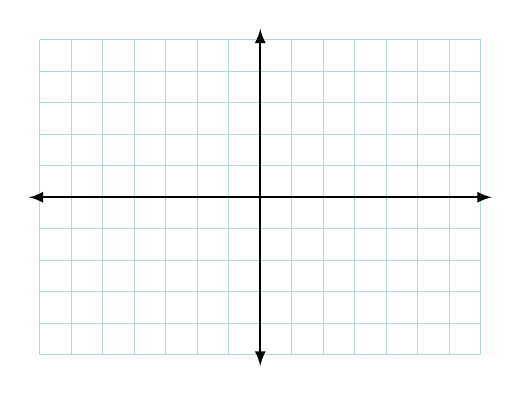
\begin{tikzpicture}[xscale=.4,yscale=.4]
          \draw[step=1,style=help lines,] (-7,-5) grid (7,5);
          \draw[latex-latex, thick] (-7.35,0)--(7.35,0);
          \draw[latex-latex, thick] (0,-5.35)--(0,5.35);
    \end{tikzpicture} & & & \\\hline
    $\displaystyle\lim_{x\to 0}x^2-2x+1$ & 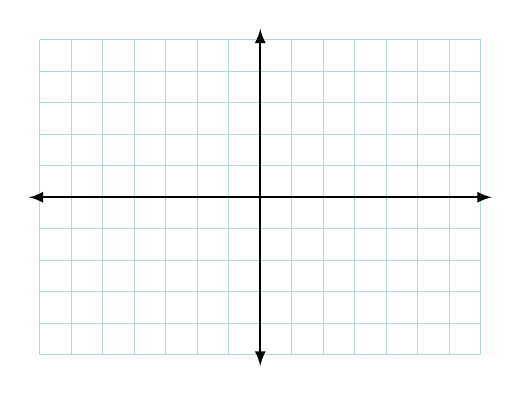
\begin{tikzpicture}[xscale=.4,yscale=.4]
          \draw[step=1,style=help lines,] (-7,-5) grid (7,5);
          \draw[latex-latex, thick] (-7.35,0)--(7.35,0);
          \draw[latex-latex, thick] (0,-5.35)--(0,5.35);
    \end{tikzpicture} & & & \\\hline
    $\displaystyle\lim_{x\to 2}\frac{x+3}{x+2}$ & 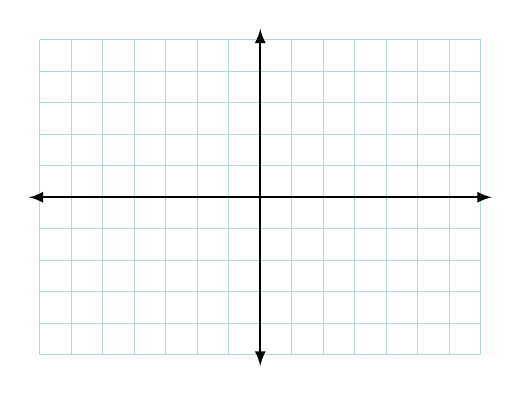
\begin{tikzpicture}[xscale=.4,yscale=.4]
          \draw[step=1,style=help lines,] (-7,-5) grid (7,5);
          \draw[latex-latex, thick] (-7.35,0)--(7.35,0);
          \draw[latex-latex, thick] (0,-5.35)--(0,5.35);
    \end{tikzpicture} & & & \\\hline
    $\displaystyle\lim_{x\to\frac{3\pi}{2}}\sin x$ & 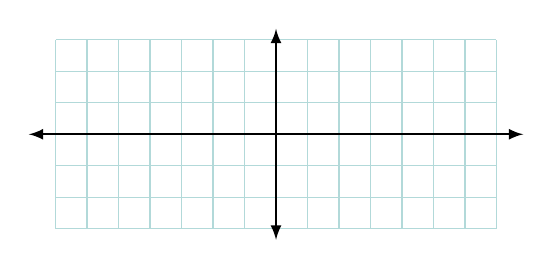
\begin{tikzpicture}[xscale=.4,yscale=.4]
          \draw[step=1,style=help lines,] (-7,-3) grid (7,3);
          \draw[latex-latex, thick] (-7.85,0)--(7.85,0);
          \draw[latex-latex, thick] (0,-3.35)--(0,3.35);
    \end{tikzpicture} & & & \\\hline
    $\displaystyle\lim_{x\to\pi}-3\cos\theta$ & 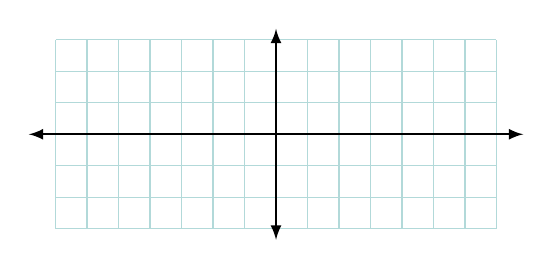
\begin{tikzpicture}[xscale=.4,yscale=.4]
          \draw[step=1,style=help lines,] (-7,-3) grid (7,3);
          \draw[latex-latex, thick] (-7.85,0)--(7.85,0);
          \draw[latex-latex, thick] (0,-3.35)--(0,3.35);
    \end{tikzpicture} & & & \\\hline
    $\displaystyle\lim_{x\to 5}\frac{x^2-25}{x-5}$ & 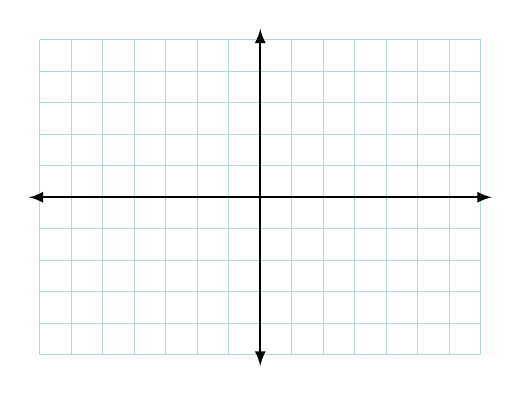
\begin{tikzpicture}[xscale=.4,yscale=.4]
          \draw[step=1,style=help lines,] (-7,-5) grid (7,5);
          \draw[latex-latex, thick] (-7.35,0)--(7.35,0);
          \draw[latex-latex, thick] (0,-5.35)--(0,5.35);
    \end{tikzpicture} & & & \\\hline
    $\displaystyle\lim_{x\to 5}|x+2|-1$ & 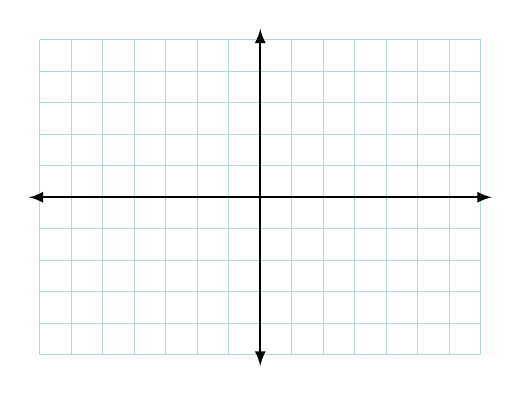
\begin{tikzpicture}[xscale=.4,yscale=.4]
          \draw[step=1,style=help lines,] (-7,-5) grid (7,5);
          \draw[latex-latex, thick] (-7.35,0)--(7.35,0);
          \draw[latex-latex, thick] (0,-5.35)--(0,5.35);
    \end{tikzpicture} & & & \\\hline
    $\displaystyle\lim_{x\to0}\frac{1}{x}$ & 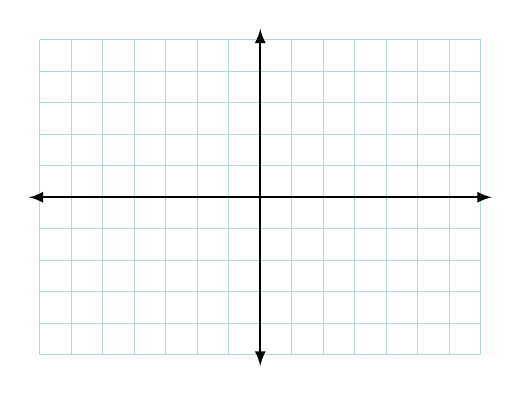
\begin{tikzpicture}[xscale=.4,yscale=.4]
          \draw[step=1,style=help lines,] (-7,-5) grid (7,5);
          \draw[latex-latex, thick] (-7.35,0)--(7.35,0);
          \draw[latex-latex, thick] (0,-5.35)--(0,5.35);
    \end{tikzpicture} & & & \\\hline
\end{longtable}
\vspace{\stretch{1}}
In short, we can interpret the limit as the expected $y$-value of a function. It doesn't really matter if the function even attains a the value the limit takes on. The behavior of the graph \textit{around} that point determines everything.
\vspace{\stretch{1}}

\newpage

\begin{tcolorbox}[title= DEFINITION OF THE EXISTENCE OF A LIMIT,colframe=black,sharp corners,colback=white,colbacktitle=white,coltitle=black,boxrule=1pt]

    A funciton has a limit as $x$ approaches $c$ if and only if the right hand limit and the left hand limit at a point $c$ are the same. That is
    
    \[\text{if }\lim_{x\to c^-}f(x)=\lim_{x\to c^+}f(x)=L,\,\text{then }\lim_{x\to c}=L.\]
\end{tcolorbox}
\vspace{.3cm}
\noindent There are three cases:
\begin{enumerate}
    \item A continuous function on the interval $(-\infty,
    ,\infty)$. \vspace{.75cm}
    \item A non-continuous function where $f(c)$ does not exist. \vspace{.75cm}
    \item A non-continuous function where $f(c)$ is defined at a different point.\vspace{.75cm}
\end{enumerate}

\noindent\textbf{Example:} Graph the function.\\
\begin{minipage}{0.30\linewidth}
    \[f(x)=
        \begin{cases}
        2-2x        &   [0,\,1)\\
        -(x-3)^2+2  &   [2,\,4)\\
        -1          &   4\\
        x-4         &   (4,\,5]
        \end{cases}
    \]
\end{minipage}
\hfill
\begin{minipage}{0.65\linewidth}
    \begin{center}
        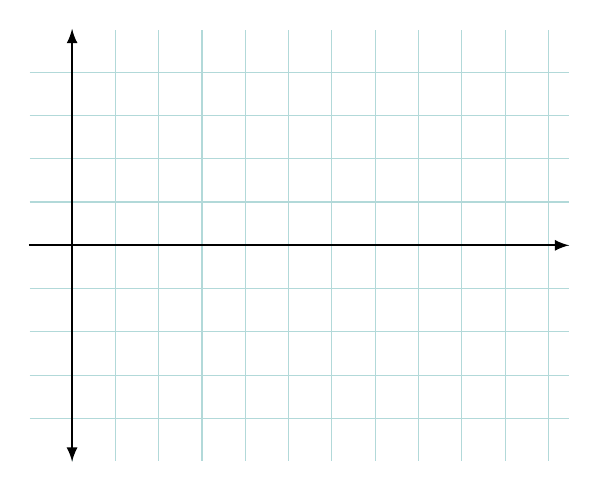
\begin{tikzpicture}[scale=1.1]
          \draw[step=.5,style=help lines] (-.49,-2.49) grid (5.74,2.49);
          \draw[-latex, thick] (-.5,0)--(5.74,0);
          \draw[latex-latex, thick] (0,-2.5)--(0,2.5);
    \end{tikzpicture}
    \end{center}
\end{minipage}

\begin{longtable}{|m{3.667cm}|m{3.667cm}|m{3.667cm}|m{3.7cm}|}
    \hline
    $\displaystyle f(0)=$   &   $\displaystyle\lim_{x\to0^+}f(x)=$  &   $\displaystyle\lim_{x\to0^-}f(x)=$  &   $\displaystyle\lim_{x\to0}f(x)=$ \\
                            &   &   &   \\\hline
    $\displaystyle f(1)=$   &   &   &   \\
                            &   &   &   \\\hline
    $\displaystyle f(2)=$   &   &   &   \\\
                            &   &   &   \\\hline
    $\displaystyle f(3)=$   &   &   &   \\\
                            &   &   &   \\\hline
    $\displaystyle f(4)=$   &   &   &   \\\
                            &   &   &   \\\hline
    $\displaystyle f(5)=$   &   &   &   \\
                            &   &   &   \\\hline
\end{longtable}

\newpage

A limit is the value of the function we \textbf{approach} as we near a particular $x$ from either the left or the right. A limit is \textbf{not} necessarily the value of the function at that point.
\vspace{\stretch{.15}}

\noindent\textbf{Strategies for Finding Limits:}
\begin{enumerate}
    \item Substitute in
    \item Simplify the equation algebraically, then substitute in
    \item Make the graph and determine the limit visually
    \item Construct a table of values to conjecture a limit
\end{enumerate}
\vspace{\stretch{.15}}
\noindent\textbf{Examples:}
\begin{questions}
    \question $\displaystyle\lim_{x\to3}\frac{x^2+1}{2x}$ \vspace{\stretch{1}}
    \question $\displaystyle\lim_{x\to2}\floor*{x}$ \vspace{\stretch{1}}
    \question $\displaystyle\lim_{x\to-4.1}\floor*{x}$ \vspace{\stretch{1}}
    \question $\displaystyle\lim_{x\to3}\frac{x^2-9}{x+3}$ \vspace{\stretch{1}}
    \question $\displaystyle\lim_{t\to2}\frac{t^2-3t+2}{t^2-4}$ \vspace{\stretch{1}}

\newpage

    \question $\displaystyle\lim_{x\to0}\frac{\frac{1}{2+x}-\frac{1}{2}}{x}$ \vspace{\stretch{1}}
    \question $\displaystyle\lim_{x\to0}\frac{(2+x)^3-8}{x}$ \vspace{\stretch{1}}
\end{questions}

\phantomsection\addcontentsline{toc}{subsection}{Properties of Limits}
\subsection*{Properties of Limits}
\begin{tcolorbox}[title= PROPERTIES OF LIMITS,colframe=black,sharp corners,colback=white,colbacktitle=white,coltitle=black,boxrule=1pt]

    Let $f$ and $g$ be functions such that $\displaystyle\lim_{x\to c}f(x)=L$ and $\displaystyle\lim_{x\to c}g(x)=M$ for real numbers $L,\,M,\,c,$ and $k$. Then the following properties of limits exist:\\
    \begin{enumerate}
        \item $\displaystyle\lim_{x\to c}\left(f(x)\pm g(x)\right)=L\pm M$\\
        \item $\displaystyle\lim_{x\to c}\left(f(x)\cdot g(x)\right)=L\cdot M$\\
        \item $\displaystyle\lim_{x\to c}\left(\frac{f(x)}{g(x)}\right)=\frac{L}{M}$\\
        \item $\displaystyle\lim_{x\to c}\left(kf(x)\right)=kL$\\
        \item $\displaystyle\lim_{x\to c}\left(f(x)\right)^k=L^k$
    \end{enumerate}
   
\end{tcolorbox}

\begin{center}
\textbf{Memorize this limit:} $\displaystyle\lim_{x\to0}\frac{\sin x}{x}=1$    
\end{center}

\textbf{Examples:}
\begin{questions}
    \question $\displaystyle\lim_{x\to0}\frac{\tan x}{x}$\vspace{\stretch{1}}
    \question $\displaystyle\lim_{x\to0}\frac{x+\sin x}{x}$\vspace{\stretch{1}}
\end{questions}



\newpage
\phantomsection\addcontentsline{toc}{subsection}{Limits Involving Infinity}
\subsection*{Limits Involving Infinity}
There are two kinds: one where the answer is infinity and one where you are finding the limit as $x$ approaches infinity.
\begin{questions}
    \begin{minipage}{0.45\linewidth}
    \question $\displaystyle\lim_{x\to2^-}\frac{1}{x-2}$
    \end{minipage}
    \hfill
    \begin{minipage}{0.45\linewidth}
    \question $\displaystyle\lim_{x\to2^+}\frac{1}{x-2}$
    \end{minipage}
    
    \vspace{\stretch{1}}
    
    \begin{minipage}{0.45\linewidth}
    \question $\displaystyle\lim_{x\to2}\frac{1}{x-2}$
    \end{minipage}
    \hfill
    \begin{minipage}{0.45\linewidth}
    \question $\displaystyle\lim_{x\to\infty}\frac{1}{x-2}$
    \end{minipage}
    
    \vspace{\stretch{1}}
\end{questions}
For problems involving polynomial and rational functions, we can determine the result of the limit without sketching the graph. Always consider the \textbf{dominant term} when evaluating.

\begin{questions}
    \question $\displaystyle\lim_{x\to\infty}x^3+2x+1$\vspace{\stretch{1}}
    \question $\displaystyle\lim_{x\to\infty}-x^3+x^2+1$\vspace{\stretch{1}}
    \question $\displaystyle\lim_{x\to\infty}\frac{7x^3}{x^3-3x^2+6x}$\vspace{\stretch{1}}
\end{questions}

\newpage

\begin{tcolorbox}[title= SHORTCUT FOR EVALUATING LIMITS AT INFINITY,colframe=black,sharp corners,colback=white,colbacktitle=white,coltitle=black,boxrule=1pt]

    Let $\displaystyle\frac{f(x)}{g(x)}$ be a rational function.
    \begin{enumerate}
        \item If $\deg f(x)>\deg g(x)$, then $\displaystyle\lim_{x\to\infty}\frac{f(x)}{g(x)}=\infty$ or $-\infty$.
        \item If $\deg f(x)<\deg g(x)$, then $\displaystyle\lim_{x\to\infty}\frac{f(x)}{g(x)}=0$.
        \item If $\deg f(x)=\deg g(x)$, then $\displaystyle\lim_{x\to\infty}\frac{f(x)}{g(x)}=\frac{a}{b}$ where $a$ and $b$ are the leading coefficients of $f(x)$ and $g(x)$ respectively.
    \end{enumerate}
   
\end{tcolorbox}
\vspace{.15cm}
\noindent\textbf{Examples:}
\begin{questions}
    \begin{minipage}{0.45\linewidth}
    \question $\displaystyle\lim_{x\to \infty}\frac{3x^3-x+1}{x+3}$
    \end{minipage}
    \hfill
    \begin{minipage}{0.45\linewidth}
    \question $\displaystyle\lim_{x\to\infty }\frac{1}{x^2}$
    \end{minipage}
    
    \vspace{\stretch{1}}
    
    \begin{minipage}{0.45\linewidth}
    \question $\displaystyle\lim_{x\to\infty}\frac{3x^2+5}{2x^2+x+3}$
    \end{minipage}
    \hfill
    \begin{minipage}{0.45\linewidth}
    \question $\displaystyle\lim_{x\to \infty}\sqrt{\frac{x+1}{x}}$
    \end{minipage}
    
    \vspace{\stretch{1}}
    
\end{questions}


\begin{tcolorbox}[title= LIMITS AND ASYMPTOTES,colframe=black,sharp corners,colback=white,colbacktitle=white,coltitle=black,boxrule=1pt]

    If $\displaystyle\lim_{x\to a^-}f(x)=\pm\infty$ or if $\displaystyle\lim_{x\to a^+}f(x)=\pm\infty$, then the line $x=a$ is a \textbf{vertical asymptote} of the graph $f(x)$.\\
    
    If $\displaystyle\lim_{x\to\infty}f(x)=b$ or if $\displaystyle\lim_{x\to -\infty}f(x)=b$, then the line $y=b$ is a \textbf{horizontal asymptote} of the graph $f(x)$.
    
    
   
\end{tcolorbox}


\newpage
\phantomsection\addcontentsline{toc}{subsection}{Continuity}
\subsection*{Continuity}
\begin{tcolorbox}[title= TEST FOR CONTINUITY,colframe=black,sharp corners,colback=white,colbacktitle=white,coltitle=black,boxrule=1pt]

    A function $f(x)$ is \textbf{continuous} on a given interval if and only if all three of the following are true:
    \begin{enumerate}
        \item $\displaystyle f(c)$ exists
        \item $\displaystyle\lim_{x\to c}f(x)$ exists
        \item $\displaystyle\lim_{x\to c}f(x)=f(c)$.
    \end{enumerate}
    If the above is not true, then we say $c$ is a \textbf{point of discontinuity}.
\end{tcolorbox}

\noindent\textbf{Examples:}
\begin{questions}
    \begin{minipage}{0.45\linewidth}
    \question $\displaystyle f(x)=x^2 +2x-8$
    \end{minipage}
    \hfill
    \begin{minipage}{0.45\linewidth}
    \question $\displaystyle f(x)=\frac{x^2-9}{x-3}$
    \end{minipage}
    
    \vspace{\stretch{1}}
    
    \begin{minipage}{0.45\linewidth}
    \question $\displaystyle f(x)=\frac{1}{x+5}$
    \end{minipage}
    \hfill
    \begin{minipage}{0.45\linewidth}
    \question $\displaystyle f(x)=\floor*{x}$
    \end{minipage}
    
    \vspace{\stretch{1}}
\end{questions}

\textbf{There are 4 kinds of discontinuity:}\hspace{2cm}\textit{Match 1-3 with the examples above}\\
\begin{questions}
\begin{minipage}{0.23\linewidth}
    \question Jump\\ Discontinuity
\end{minipage}
\hfill
\begin{minipage}{0.23\linewidth}
    \question Infinite\\ Discontinuity
\end{minipage}
\hfill
\begin{minipage}{0.23\linewidth}
    \question Removable\\ Discontinuity
\end{minipage}
\hfill
\begin{minipage}{0.23\linewidth}
    \question Oscillating\\ Discontinuity*
\end{minipage}
\end{questions}
\vspace{.4cm}

*Oscillating Discontinuities are rare in the scope of this course, but worth noting nonetheless. To see an example, check out the graph of the \textbf{Topologist's Sine Curve}, $y=\sin\left(\frac{1}{x}\right)$.


\newpage

\begin{tcolorbox}[title= PROPERTIES OF CONTINUOUS FUNCTIONS,colframe=black,sharp corners,colback=white,colbacktitle=white,coltitle=black,boxrule=1pt]

    If $f$ and $g$ are continuous at $x=c$, then the following combinations are continuous at $x=c$.
    \begin{enumerate}
        \item $f\pm g$
        \item $f\cdot g$ 
        \item $k\cdot f$ for any scalar $k$
        \item $\frac{f}{g}$ when $g(c)\ne0$
        \item $f\circ g$ or $f(g(x))$ if $f$ is continuous at $g(c)$.
    \end{enumerate}
\end{tcolorbox}
\vspace{.15cm}
\begin{questions}
    \question Explain how the function $\displaystyle y=\left|\frac{x\sin x}{x^2+1}\right|$ is always continuous.
    \vspace{\stretch{1}}
    \question Find a value of $a$ so that the function $f(x)=\begin{cases}
    2x+3 & x\le2\\
    ax+1 & x>2
    \end{cases}$ is continuous.
    \vspace{\stretch{1}}
\end{questions}

\phantomsection\addcontentsline{toc}{subsection}{Intermediate Value Theorem}
\subsection*{Intermediate Value Theorem}
\begin{tcolorbox}[title= THE INTERMEDIATE VALUE THEOREM,colframe=black,sharp corners,colback=white,colbacktitle=white,coltitle=black,boxrule=1pt]

    A function $y=f(x)$ that is continuous on a closed interval $[a,\,b]$ takes on every value between $f(a)$ and $f(b)$. In other words, if $f(a)\le y_0\le f(b)$, then $y_0=f(c)$ for some $c\in[a,\,b]$.
\end{tcolorbox}
\vspace{.15cm}
\noindent\textbf{Examples:}
\begin{questions}
    \question Apply the IVT to verify the existence of a point where $f(x)=0$ on the interval $[0,\,5]$ given $f(x)=x^3-2x-2$.
    \vspace{\stretch{.7}}
    \question Is there a real number that is exactly one more than its cube? Justify your answer.
    \vspace{\stretch{.7}}
\end{questions}



\newpage
\phantomsection\addcontentsline{toc}{subsection}{Rates of Change \& Tangent Lines}
\subsection*{Rates of Change \& Tangent Lines}

The \textbf{average rate of change} of a quantity over a period of time is the amount of change divided by the time it takes. This is just a fancy way of describing the \textbf{slope}.\\
\\
\noindent\textbf{Example:} Find the average rate of change in the population of fruit flies from day 23 to day 45.

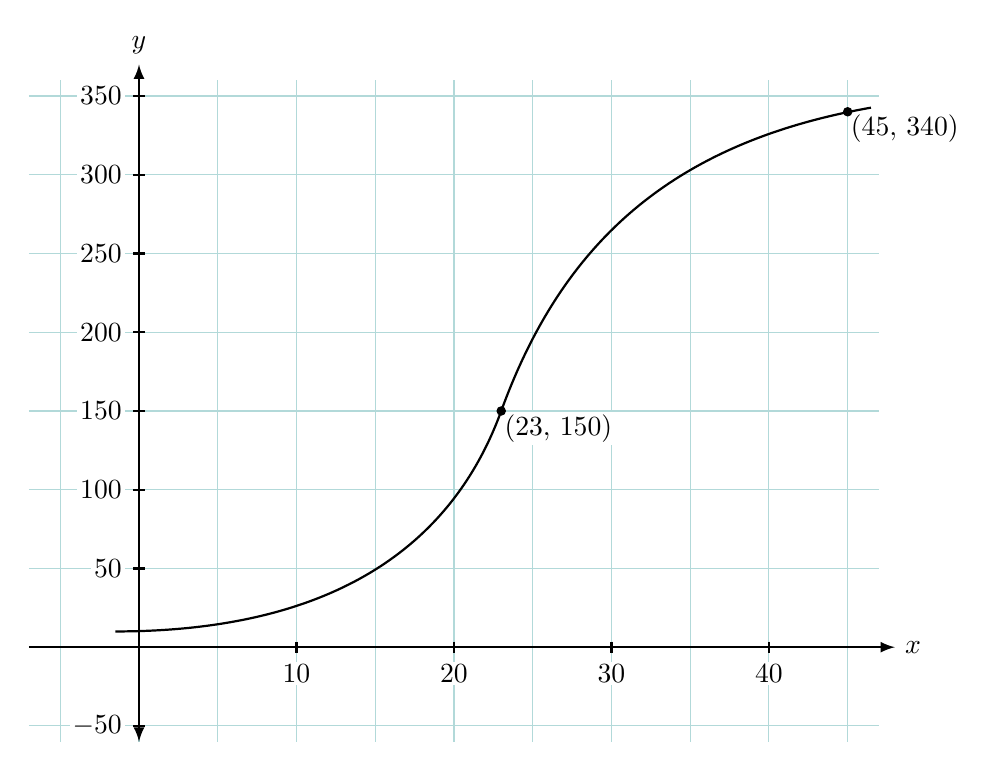
\begin{tikzpicture}[xscale=.20,yscale=.20]
    \draw[step=5,style=help lines,] (-7,-6) grid (47,36);
    \draw[-latex, thick] (-7,0)--(48,0) node[right]{$x$};
    \draw[latex-latex, thick] (0,-6)--(0,37) node[above]{$y$};
    
    \foreach \x/\xtext in {10,20,30,40} \draw[shift={(\x,0)},thick] (0pt,10pt) -- (0pt, -10pt) node[below=1mm,fill=white,inner sep=1pt]{$\xtext$};
    
    \foreach \y/\ytext in {5,10,15,20,25,30,35,-5} \draw[shift={(0,\y)},thick] (10pt,0pt) -- (-10pt, 0pt) node[left=1mm,fill=white,inner sep=1pt]{$\ytext0$};
  
    
    \node at (23,15)[anchor=north west,fill=white,inner sep=1pt]{$(23,\,150)$};
    \node at (45,34) [anchor=north west,fill=white,inner sep=1pt] {$(45,\,340)$};
    \node[circle,draw=black, fill=black, inner sep=0pt,minimum size=3pt] at (23,15) {};
    \node[circle,draw=black, fill=black, inner sep=0pt,minimum size=3pt] at (45,34) {};
    
    \draw[-,thick,shorten <=-.3cm] (0,1) to [out=0,in=250] (23,15);
    \draw[-,thick,shorten >=-.3cm] (23,15) to[out=70,in=-170] (45,34);
\end{tikzpicture}

A line through two points on a curve is called a \textbf{secant} to the curve. The slope of the secant line is the average rate of change.\\
\\
\\
\\
Did the number of flies increase by 8.6 each day?\\
\\
\\
\\
How fast was the fly population growing on day 23?

\newpage

The population growth on one particular day poses a problem: it would be the slope of the line at \textit{only one point}. We need \textit{two} points to use the slope formula as we know it. How do we circumvent this issue?\\
\\
\\
\textbf{Example:} Given $y=x^2$, what is the average rate of change on $[0,\,3]$?

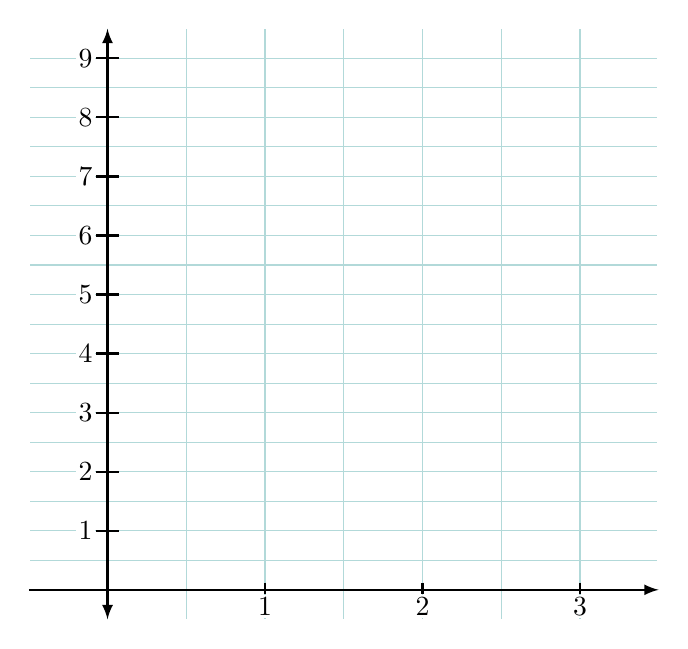
\begin{tikzpicture}[xscale=2,yscale=.75]
  \draw[step=.5,style=help lines] (-.49,-.49) grid (3.49,9.49);
  \draw[-latex, thick] (-.5,0)--(3.5,0);
  \draw[latex-latex, thick] (0,-.5)--(0,9.5);
  
  \foreach \x/\xtext in {1,2,3} \draw[shift={(\x,0)},thick] (0pt,3.5pt) -- (0pt, -2pt) node[below,fill=white,inner sep=1pt]{$\xtext$};
    
  \foreach \y/\ytext in {1,2,3,4,5,6,7,8,9} \draw[shift={(0,\y)},thick] (2pt,0pt) -- (-2pt, 0pt) node[left,fill=white,inner sep=1pt]{$\ytext$};
  
\end{tikzpicture}

What is the instantaneous rate of change at $x=1$?

\newpage


\begin{tcolorbox}[title= DEFINITION OF TANGENT LINE WITH SLOPE \textit{m},colframe=black,sharp corners,colback=white,colbacktitle=white,coltitle=black,boxrule=1pt]

    If $f$ is defined on an open interval containing $c$, and if the limit
    \[\lim_{\Delta x\to0}\frac{\Delta y}{\Delta x}=\lim_{\Delta x\to0}\frac{f(c+\Delta x)-f(c)}{\Delta x}=m\]
    exists, then the line passing through $(c,\,f(c))$ with slope $m$ is the \textbf{tangent line} to the graph of $f$ at the point $(c,\,f(c))$.
    
\end{tcolorbox}
\vspace{.15cm}
\noindent\textbf{Examples:}
\begin{questions}
    \question Write the equation of the tangent line to the curve $f(x)=3x^2+1$ at $x=-1$. 
    \vspace{\stretch{1}}
    
    \question Write a general formula for the slope of the tangent line to $f(x)=2x^2-x$ for any point $x=a$.
    \vspace{\stretch{1}}
    
    \question Write an equation for the line \textbf{normal} to the curve $f(x)=4-x^2$ at $x=1$.
    \vspace{\stretch{1}}
    
    \question Find the equations of all lines tangent to $y=9-x^2$ that pass through $(1,\,12)$.
    \vspace{\stretch{1.2}}
\end{questions}


\newpage
\phantomsection\addcontentsline{toc}{section}{Derivatives}
\phantomsection\addcontentsline{toc}{subsection}{Definition of the Derivative}
\subsection*{Definition of the Derivative}
\begin{tcolorbox}[title= DEFINITION OF THE DERIVATIVE OF A FUNCTION,colframe=black,sharp corners,colback=white,colbacktitle=white,coltitle=black,boxrule=1pt]

    The \textbf{derivative} of $f$ at $x$ is given by
    \[f'(x)=\lim_{\Delta x\to0}\frac{f(x+\Delta x)-f(x)}{\Delta x}\]
    provided the limit exists. For all $x$ for which this limit exists, $f'$ is a function of $x$.
    
\end{tcolorbox}
\vspace{.15cm}
\begin{center}
    \textbf{The derivative of a function is the formula for the slope of the tangent line.}
\end{center}
\noindent\textbf{Examples:} Compute the derivatives of the following functions. \textit{Note that these require some algebraic tricks to compute.}
\begin{questions}
    \question $\displaystyle f(x)=\sqrt{x-3}$
    \vspace{\stretch{1}}
    
    \question $\displaystyle f(x)=\frac{1}{x-5}$
    \vspace{\stretch{1}}
\end{questions}



\newpage
\phantomsection\addcontentsline{toc}{subsection}{Rules for Differentiation A}
\subsection*{Rules for Differentiation A}

Let $y=f(x)$ be a function of $x$. If the limit $\displaystyle\lim_{\Delta x\to0}\frac{f(x+\Delta x)-f(x)}{\Delta x}$ exists and is finite, we call this limit the derivative of $f$ at $x$ and say that $f$ is \textit{differentiable} at $x$.

\noindent\textbf{Rules for Differentiation:}
\begin{questions}
    \question \textbf{Constant Rule:}
    \begin{parts}
        \part $\displaystyle y=5$
    \end{parts}
    
    \question \textbf{Power Rule:}
    \begin{parts}
        \part $\displaystyle y=x^2$
        \part $\displaystyle f(x)=x^3$
        \part $\displaystyle \frac{d}{dx}\left(x^4\right)=$
        \part $\displaystyle y=x^{13}$
        \part $\displaystyle \frac{d}{dx}\left(x^{79}\right)=$
    \end{parts}
    
    \question \textbf{Constant Multiple Rule:}
    \begin{parts}
        \part $\displaystyle \frac{d}{dx}\left(7x^5\right)=$
        \part $\displaystyle y=-3x^4$
        \part $\displaystyle \frac{d}{dx}\left(\frac{2}{3}x^3\right)=$
    \end{parts}
    
    \question \textbf{Sum and Difference Rule:}
    \begin{parts}
        \part $\displaystyle \frac{d}{dx}\left(x^3+7x^2-5x+4\right)=$
        \part $\displaystyle y= \frac{1}{4}x^4-\frac{x^3}{3}+4$
    \end{parts}
    
    \question \textbf{Higher Order Derivatives:}
    \begin{parts}
        \part $\displaystyle y=x^3-5x^2+2$\vspace{\stretch{1}}
        
        \part $\displaystyle y=\frac{x+1}{x}$
        \vspace{\stretch{1}}
    \end{parts}
\end{questions}


\newpage

For a derivative to exist, the left-hand and right-hand derivatives must be the same in order for there to be derivative at that point \textit{and} for derivatives, it must be continuous at that point.
\begin{questions}
    \question Determine whether the curve has a tangent at the indicated point. If it does, give the slope at that point. If not, explain why.
    \begin{parts}
        \part $\displaystyle f(x)=\begin{cases}
        -x      & x<0\\
        x^2-x   & x\ge0
        \end{cases}$ at $x=0$
        \vspace{\stretch{1}}
        \part $\displaystyle f(x)=\begin{cases}
        \sin x      & 0\le x<3\pi/4\\
        \cos x   & 3\pi/4\le x\le 2\pi
        \end{cases}$ at $x=3\pi/4$
        \vspace{\stretch{1}}
    \end{parts}
    \question True or False: The graph of $f(x)=|x|$ has a tangent line at x=0. Justify your answer.
    \vspace{\stretch{.67}}
\end{questions}



\newpage
\phantomsection\addcontentsline{toc}{subsection}{Rules for Differentiation B}
\subsection*{Rules for Differentiation B}
\noindent\textbf{More Rules:}
\begin{questions}
    \question \textbf{Product Rule:} $\displaystyle\frac{d}{dx}(uv)=v\cdot\frac{du}{dx}+u\cdot\frac{dv}{dx}$
    \begin{parts}
        \part $y=(3x-1)(2x+5)$\vspace{.5cm}
        \part $f(x)=(1+x^2)(-3x-4)$\vspace{.5cm}
    \end{parts}
    \question \textbf{Quotient Rule:} $\displaystyle\frac{d}{dx}\left(\frac{u}{v}\right)=\frac{v\cdot\frac{du}{dx}-u\cdot\frac{dv}{dx}}{v^2}$
    \begin{parts}
        \part $\displaystyle y=\frac{x^2+1}{x^2-1}$\vspace{.5cm}
        \part $\displaystyle \frac{d}{dx}\left(\frac{x^2}{1-x^3}\right)=$\vspace{.5cm}
    \end{parts}
    \question \textbf{Extended Power Rule:} $\displaystyle\frac{d}{dx}\left(u^n\right)=nu^{n-1}\cdot\frac{du}{dx}$
    \begin{parts}
        \part $\displaystyle y=(x^2-3x+1)^5$\vspace{.5cm}
        \part $\displaystyle f(x)=\left(x^2+1\right)^-2$\vspace{.5cm}
        \part $\displaystyle\frac{d}{dx}\left[(x^2+1)^3(x-1)^2\right]=$\vspace{.5cm}
    \end{parts}
\end{questions}

\noindent\textbf{Examples:} Make sure to choose the \textit{correct} strategy!
\begin{questions}
    \begin{minipage}{0.45\linewidth}
    \question $\displaystyle y=\frac{1}{(x^2-1)^5}$
    \end{minipage}
    \hfill
    \begin{minipage}{0.45\linewidth}
    \question $\displaystyle\frac{d}{dx}\left(\frac{2x-1}{x+7}\right)^3=$
    \end{minipage}
    
    \newpage
    
    \question $\displaystyle g(x)=\frac{(x-1)(x^2-2x)}{x^4}$
    \vspace{\stretch{1}}
    
    \question Let $u$ and $v$ be functions that are differentiable at $x=2$ and that $u(2)=3,\,u'(2)=-4,\,v(2)=1,$ and $v'(2)=2$. Find the values of the following derivatives at $x=2$.
    \begin{parts}
        \part $\displaystyle\frac{d}{dx}(uv)=$
        \vspace{\stretch{1}}
        \part $\displaystyle\frac{d}{dx}\left(\frac{u}{v}\right)=$
        \vspace{\stretch{1}}
        \part $\displaystyle\frac{d}{dx}\left(\frac{v}{u}\right)=$
        \vspace{\stretch{1}}
    \end{parts}
    
\end{questions}



\newpage
\phantomsection\addcontentsline{toc}{subsection}{Distance, Velocity, \& Acceleration}
\subsection*{Distance, Velocity, \& Acceleration}
\noindent\textbf{Distance:} The function $s(t)$ gives the position $s$ on a line as a function of time $t$.\\
\noindent\textbf{Displacement:} The displacement of an object over the time interval from $t$ to $t+\Delta t$ is $\Delta s=f(t+\Delta t)-f(t)$.\\
\noindent\textbf{Velocity:} The derivative of the position equation is velocity because it describes how fast the position is changing. $v(t)=s'(t)$
\begin{questions}
    \question Average Velocity: the average velocity over a period of time. $\displaystyle\frac{\Delta s}{\Delta t}$, where $\Delta s$ represents \textbf{displacement} and $\Delta t$ represents the \textbf{time traveled}.
    \vspace{.1cm}
    \question Instantaneous Velocity: how fast \textbf{and in what direction} an object is moving at a given instant.
    \begin{parts}
        \part Velocity is \textbf{positive} when the object is moving forward or up and the distance is increasing.
        \part Velocity is \textbf{negative} when the object is moving back or down and the distance is decreasing.
    \end{parts}
    \question Speed: how fast an object is moving at a given instant, $\displaystyle |v(t)|=\left|\frac{ds}{dt}\right|$. The only difference between velocity and speed is that velocity includes \textbf{direction}.
\end{questions}
\noindent\textbf{Acceleration:} The derivative of the velocity equation is acceleration because it describes \textbf{how fast the velocity is changing}. $\displaystyle a(t)=\frac{dv}{dt}=\frac{d^2 s}{dt^2}$\\
\\
\noindent\textbf{Examples:}\\
For each of the following, $s$ represents the position of a moving body with $s$ in feet and $t$ in seconds. Find the body's velocity and acceleration.
\begin{questions}
    \question $s(t)=16t^2+3$
    \vspace{\stretch{1}}
    \question $s(t)=832t-16t^2$
    \vspace{\stretch{1}}
    
    \newpage
    
    
    \question The position of a body at time $t$ is $s=t^3-4t^2-3t$. Find the acceleration each time the velocity is zero.
    \vspace{\stretch{1}}
    
    \question A particle moves along a line so that its position at any time $t\ge0$ is given by the function $s(t)=t^2-4t+3$, where $s$ is measured in meters and $t$ is measured in seconds.
    \begin{parts}
        \part Find the displacement in the first 2 seconds.
        \part Find the average velocity in the first 4 seconds.
        \part Find the instantaneious velocity when $t=4$.
        \part Find the acceleration when $t=4$.
        Describe the motion of the particle. At what values of $t$ does the particle change direction?
        \part Where is the particle when $s$ is a minimum?
        \vspace{\stretch{1}}
    \end{parts}
    
    \question A ball is thrown vertically upward at a speed of 30 m/s. Its height in meters $t$ seconds later is given by $h(t)=30t-5t^2$.
    \begin{parts}
        \part Find the maximum height of the ball.
        \part Find the acceleration of the ball.
    \end{parts}
    \vspace{\stretch{.80}}
\end{questions}


\newpage
\phantomsection\addcontentsline{toc}{subsection}{Derivatives of Sine and Cosine}
\subsection*{Derivatives of Sine and Cosine}
Below is the graph of $y=\sin x$. Using the fact that $y'$ is the slope of the tangent line, make the graph of $y'$ for $y=\sin x$.
\begin{center}
    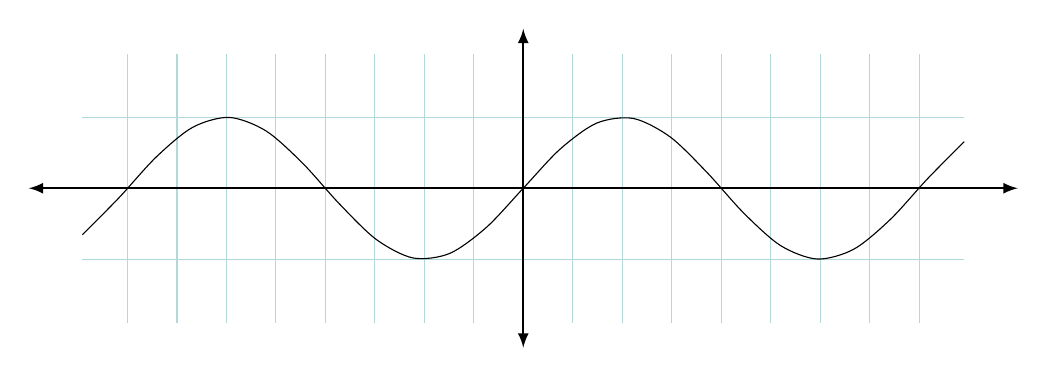
\begin{tikzpicture}[xscale=.8,yscale=.9]
          \draw[ystep=1,xstep=pi/4,style=help lines,] (-7,-1.9) grid (7,1.9);
          \draw[latex-latex, thick] (-7.85,0)--(7.85,0);
          \draw[latex-latex, thick] (0,-2.25)--(0,2.25);
          \draw[domain=-7:7, smooth] plot (\x, {sin(\x r)});
    \end{tikzpicture}
\end{center}

Similarly, attempt with the graph of $y=\cos x$.
\begin{center}
    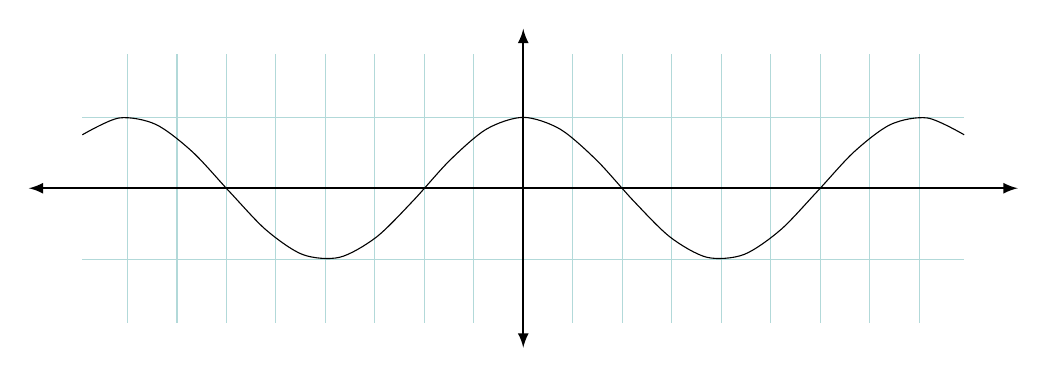
\begin{tikzpicture}[xscale=.8,yscale=.9]
          \draw[ystep=1,xstep=pi/4,style=help lines,] (-7,-1.9) grid (7,1.9);
          \draw[latex-latex, thick] (-7.85,0)--(7.85,0);
          \draw[latex-latex, thick] (0,-2.25)--(0,2.25);
          \draw[domain=-7:7, smooth] plot (\x, {cos(\x r)});
    \end{tikzpicture}
\end{center}
\vspace{.05cm}
\begin{tcolorbox}[title= DERIVATIVES OF SINE AND COSINE,colframe=black,sharp corners,colback=white,colbacktitle=white,coltitle=black,boxrule=1pt]

    \begin{align*}
        \frac{d}{dx}(\sin x) &= \hspace{1.5cm} & \frac{d}{dx}(\cos x) &= \hspace{1.5cm}
    \end{align*}
    \vspace{.05cm}
\end{tcolorbox}
\vspace{.15cm}
\noindent\textbf{Examples:}
Find the derivative of each of the following.
\begin{questions}
    \begin{minipage}{0.3\linewidth}
    \question $\displaystyle y=2\sin x$
    \end{minipage}
    \hfill
    \begin{minipage}{0.3\linewidth}
    \question $\displaystyle f(x)=\frac{-\sin x}{10}$
    \end{minipage}
    \hfill
    \begin{minipage}{0.3\linewidth}
    \question $\displaystyle u=x+\cos x$
    \end{minipage}
\end{questions}

\newpage
\phantomsection\addcontentsline{toc}{subsection}{The Chain Rule}
\subsection*{The Chain Rule}
In your head, consider the derivative of the function $y=(3x+4)^2$. To do it, we have to "take the derivative of the inside". More formally, this is another differentiation rule that we call the \textbf{Chain Rule}.\\

\begin{tcolorbox}[title= THE CHAIN RULE,colframe=black,sharp corners,colback=white,colbacktitle=white,coltitle=black,boxrule=1pt]

    If $y=f(u)$ is a differentiable function of $u$ and $u=g(x)$ is a differentiable function of $x$, then $y=f(g(x))$ is a differentiable function of $x$ and 
    \[\frac{dy}{dx}=\frac{dy}{du}\cdot\frac{du}{dx}\]
    or, equivalently
    \[\frac{d}{dx}\left(f(g(x))\right)=f'(g(x))\cdot g'(x).\]
    
\end{tcolorbox}
\vspace{.15cm}
\noindent\textbf{Examples:}
\begin{questions}
    \question Suppose that functions $f$ and $g$ and their derivatives have the following values at $x=2$ and $x=3$.
    \begin{longtable}[ht]{|C{1.5cm}|C{1.5cm}|C{1.5cm}|C{1.5cm}|C{1.5cm}|}
        \hline
        $x$\Tstrut\Bstrut & $f(x)$\Tstrut\Bstrut & $g(x)$\Tstrut\Bstrut & $f'(x)$\Tstrut\Bstrut & $g'(x)$\Tstrut\Bstrut\\\hline
        $2$\Tstrut\Bstrut & $8$\Tstrut\Bstrut & $2$\Tstrut\Bstrut & $1/3$\Tstrut\Bstrut & $-3$\Tstrut\Bstrut\\\hline
        $3$\Tstrut\Bstrut & $3$\Tstrut\Bstrut & $-4$\Tstrut\Bstrut & $2\pi$\Tstrut\Bstrut & $5$\Tstrut\Bstrut\\\hline
    \end{longtable}
    Evaluate  the derivatives with respect to $x$ of the following combinations at the given value of $x$
    \begin{parts}
        \begin{minipage}{.45\linewidth}
            \part $\displaystyle 2f(x),\, x=2 $
        \end{minipage}
        \hfill
        \begin{minipage}{.45\linewidth}
            \part $\displaystyle f(x)\cdot g(x),\, x=3$
        \end{minipage}
        
        \vspace{\stretch{1}}
        
        \begin{minipage}{.45\linewidth}
            \part $\displaystyle \frac{f(x)}{g(x)},\, x=2$
        \end{minipage}
        \hfill
        \begin{minipage}{.45\linewidth}
            \part $\displaystyle f(g(x)),\,x=2$
        \end{minipage}
        
        \vspace{\stretch{1}}
        
        \begin{minipage}{.45\linewidth}
            \part $\displaystyle \frac{1}{g^2(x)},\,x=3$
        \end{minipage}
        \hfill
        \begin{minipage}{.45\linewidth}
            \part $\displaystyle \sqrt{f^2(x)+g^2(x)},\,x=2$
        \end{minipage}
        
        \vspace{\stretch{1}}
    \end{parts}
    
    \newpage
    
    \question Find $\displaystyle\frac{dy}{dx}$ for the two similar functions.
    \begin{parts}
        \begin{minipage}{.45\linewidth}
            \part $\displaystyle \frac{d}{dx}\left(\sin^2 x\right)=$
        \end{minipage}
        \hfill
        \begin{minipage}{.45\linewidth}
            \part $\displaystyle \frac{d}{dx}\left(\sin x^2\right)=$
        \end{minipage}
    \end{parts}
    
    \vspace{\stretch{1}}
    
    \question $\displaystyle f(u)=\left(\frac{u-1}{u+1}\right)^2,\, g(x)=\frac{1}{x^2}-1$ and find $(f\circ g)'(-1)$.
    
    \vspace{\stretch{1}}
    
    \question Let $y=x^2+7x-5.$ Evaluate $\displaystyle\frac{dy}{dt}$ when $x=1$ and $\displaystyle\frac{dx}{dt}=\frac{1}{3}$.
    
    \vspace{\stretch{1}}
    

    
\end{questions}


\newpage
\phantomsection\addcontentsline{toc}{subsection}{Derivatives of Trigonometric Functions}
\subsection*{Derivatives of Trigonometric Functions}
\begin{tcolorbox}[title= DERIVATIVE RULES FOR ALL TRIG FUNCTIONS,colframe=black,sharp corners,colback=white,colbacktitle=white,coltitle=black,boxrule=1pt]

    \begin{align*}
        \frac{d}{dx}(\sin u) &= \cos u\frac{du}{dx} & \frac{d}{dx}(\csc u) &= -\csc u\cot u\frac{du}{dx}\\
        \frac{d}{dx}(\cos u) &= -\sin u\frac{du}{dx} & \frac{d}{dx}(\sec u) &= \sec u\tan u\frac{du}{dx}\\
        \frac{d}{dx}(\tan u) &= \sec^2 u\frac{du}{dx} & \frac{d}{dx}(\cot u) &= -\csc^2 u\frac{du}{dx}
    \end{align*}
    \vspace{.05cm}
\end{tcolorbox}
\vspace{.15cm}
Try out the following derivatives. Remember, \textbf{all other derivative rules still apply}!!
\begin{questions}
    \question $\displaystyle \frac{d}{dx}\left( \cos^2 (3x)\right)=$ \vspace{1cm}
    \question $\displaystyle \frac{d}{dx}\left( \sec^2 (5x)\right)=$\vspace{1cm}
    \question $\displaystyle \frac{d}{dx}\left( \sqrt{\tan (3x)}\right)=$\vspace{1cm}
    \question $\displaystyle \frac{d}{dx}\left( x^2\sin x\right)=$\vspace{1cm}
    \question $\displaystyle \frac{d^2}{dx^2}\left( \frac{1}{\cos x}\right)=$\vspace{\stretch{1}}
\end{questions}
\textbf{WARNING:} You are \textit{going} to need to memorize multiple trig identities for later units. You will start practicing that for tonight's homework as well.




\newpage
\phantomsection\addcontentsline{toc}{subsection}{Implicit Differentiation}
\subsection*{Implicit Differentiation}
What we have been doing so far is explicit differentiation, as $y$ has always been an explicit function of $x$. Today, we will continue our journey of taking derivatives but now with equations that are not functions!\\
\begin{tcolorbox}[title= STEPS FOR IMPLICIT DIFFERENTIATION,colframe=black,sharp corners,colback=white,colbacktitle=white,coltitle=black,boxrule=1pt]
    \begin{enumerate}
        \item Differentiate both sides of the equation with respect to $x$, doing $x$ as you normally would. The derivative of $y$ becomes $dy/dx$ or $y'$.
        \item Collect terms with $dy/dx$ on one side of the equation.
        \item Factor out the $dy/dx$.
        \item Solve for $dy/dx$.
    \end{enumerate}
\end{tcolorbox}
\vspace{.15cm}
\noindent\textbf{Examples:} Find $\displaystyle\frac{dy}{dx}$.
\begin{questions}
    \begin{minipage}{.45\linewidth}
    \question $\displaystyle y^2=x$
    \end{minipage}
    \hfill
    \begin{minipage}{.45\linewidth}
    \question $\displaystyle x^2+y^2=25$
    \end{minipage}
    
    \vspace{\stretch{.6}}
    
    \question The Folium of Descartes is $x^3+y^3=9xy$. Find and graph the tangent lines at the points $(4,\,2)$ and $(2,\,4)$.
    
    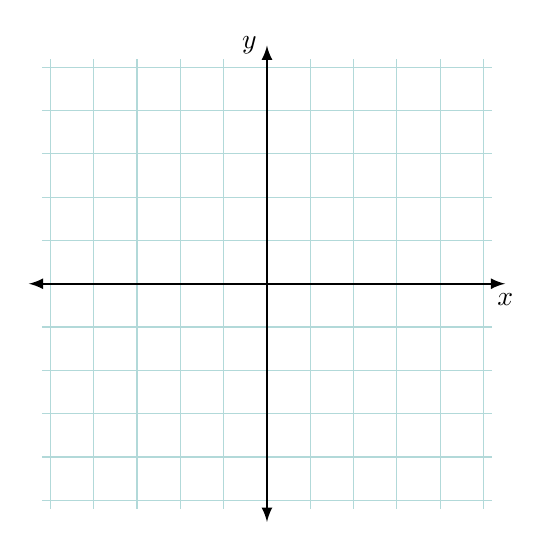
\begin{tikzpicture}[scale=.55]
        \draw[style=help lines] (-5.2,-5.2) grid (5.2,5.2);
        \draw[latex-latex,thick] (-5.5,0) -- (5.5,0) node[below] {$x$};
        \draw[latex-latex,thick] (0,-5.5) -- (0,5.5) node[left] {$y$};
        \draw[thick] plot[raw gnuplot,smooth] function {
            f(x,y) = (x**3)+(y**3)-9*x*y;
            set xrange [-5.2:5.2];
            set yrange [-5.2:5.2];
            set view 0,0;
            set isosample 500,500;
            set cont base;
            set cntrparam levels incre 0,0.1,0;
            unset surface;
            splot f(x,y);
        };
    \end{tikzpicture}
    
    \vspace{\stretch{.1}}
    
    \newpage
    
    \question The line that is normal to the curve $y=x^2+2x-3$ at $(1,\,0)$ intersects the curve at what other point?
    \vspace{\stretch{1}}
    
\end{questions}


\textbf{Example:} Find $\displaystyle\frac{d^2y}{dx^2}$ for $2x^3-3y^2=8$.
\vspace{\stretch{2}}

Second derivatives of Implicit Functions is a skill that is always exercised on the AP Exam. The level of simplification might vary, but the overall procedure and \textit{form} of the final answer is important.

\newpage

Two more examples of second derivatives (time-permitting):
\begin{questions}
    \question $\displaystyle 5y^2+2=5x^2$
    \vspace{\stretch{1}}
    
    \question $y+\cos y=x+1$
    \vspace{\stretch{1}}
\end{questions}

\newpage
\phantomsection\addcontentsline{toc}{subsection}{Derivatives of Transcendental Functions}
\subsection*{Derivatives of Transcendental Functions}
\begin{tcolorbox}[title= DERIVATIVES OF INVERSE TRIGONOMETRIC FUNCTIONS,colframe=black,sharp corners, colback=white, colbacktitle=white, coltitle=black, boxrule=1pt]
    
    Let $u$ be a differentiable function of $x$.
    \begin{align*}
        \frac{d}{dx}(\arcsin u) &= \frac{du}{\sqrt{1-u^2}} & \frac{d}{dx}(\arccos u) &= \frac{-du}{\sqrt{1-u^2}}\\
        \frac{d}{dx}(\arctan u) &= \frac{du}{1+u^2} & \frac{d}{dx}(\text{arccot } u) &= \frac{-du}{1+u^2}\\
        \frac{d}{dx}(\text{arcsec } u) &= \frac{du}{|u|\sqrt{u^2-1}} & \frac{d}{dx}(\text{arccsc } u) &= \frac{-du}{|u|\sqrt{u^2-1}}\\
    \end{align*}
\end{tcolorbox}
\vspace{.15cm}
\noindent\textbf{Examples:} Find $\displaystyle\frac{dy}{dx}$.
\begin{questions}
    \question $\displaystyle y=\sin^{-1}x^2$
    \vspace{\stretch{1}}
    
    \question $\displaystyle y=\cos^{-1}\left(\frac{1}{x}\right)$
    \vspace{\stretch{1}}
    
    \question $\displaystyle y=\cot^{-1}\sqrt{x}$
    \vspace{\stretch{1}}
    
    \question $\displaystyle y=x\sqrt{1-x^2}-\cos^{-1}x$
    \vspace{\stretch{1}}
    
    \newpage
    
    \question $\displaystyle y=x\arcsin x+\sqrt{1-x^2}$
    \vspace{\stretch{1}}
    
    \question A particle moves along the $x$-axis so that its position at any time $t\ge0$ is $x(t)=\arctan\sqrt{t}$. What is the velocity of the particle when $t=16$?
    \vspace{\stretch{1}}
\end{questions}


\begin{tcolorbox}[title= DERIVATIVES OF THE EXPONENTIAL FUNCTION,colframe=black,sharp corners, colback=white, colbacktitle=white, coltitle=black, boxrule=1pt]
    
    Let $u$ be a differentiable function of $x$.
    \begin{align*}
        \frac{d}{dx}\left(e^u\right) &= u'\cdot e^u & \frac{d}{dx}\left(a^u\right) &= u'\cdot a^u\cdot\ln a
    \end{align*}
\end{tcolorbox}
\vspace{.15cm}
\textbf{Examples:}
\begin{questions}
    \begin{minipage}{0.45\linewidth}
        \question $\displaystyle y=e^{\sin x}$
    \end{minipage}
    \hfill
    \begin{minipage}{0.45\linewidth}
        \question $\displaystyle y=e^{(x+1)}$
    \end{minipage}
    
    \vspace{\stretch{1}}
    
    \begin{minipage}{0.45\linewidth}
        \question $\displaystyle y=\cos\left(e^x\right)$
    \end{minipage}
    \hfill
    \begin{minipage}{0.45\linewidth}
        \question $\displaystyle y=(1+2x)3^{-2x}$
    \end{minipage}
    
    \vspace{\stretch{1}}
    
    \begin{minipage}{0.45\linewidth}
        \question $\displaystyle y=e^{3^x}$
    \end{minipage}
    \hfill
    \begin{minipage}{0.45\linewidth}
        \question $\displaystyle y=e^{x^2}e^{-x}$
    \end{minipage}
    
    \vspace{\stretch{1}}
\end{questions}

\newpage

\begin{tcolorbox}[title= DERIVATIVES OF THE LOGARITHMIC FUNCTION,colframe=black,sharp corners, colback=white, colbacktitle=white, coltitle=black, boxrule=1pt]
    
    Let $u$ be a differentiable function of $x$.
    \begin{align*}
        \frac{d}{dx}\left(\ln u\right) &= \frac{u'}{u} & \frac{d}{dx}\left(\log_a u\right) &= \frac{u'}{u\cdot\ln a}
    \end{align*}
\end{tcolorbox}
\vspace{.15cm}
\textbf{Examples:}
\begin{questions}
    \begin{minipage}{0.45\linewidth}
        \question $\displaystyle y=\ln(5x)$
    \end{minipage}
    \hfill
    \begin{minipage}{0.45\linewidth}
        \question $\displaystyle y=\ln(\cos x)$
    \end{minipage}
    
    \vspace{\stretch{1}}
    
    \begin{minipage}{0.45\linewidth}
        \question $\displaystyle y=\ln(\ln x)$
    \end{minipage}
    \hfill
    \begin{minipage}{0.45\linewidth}
        \question $\displaystyle y=\left(\ln x\right)^2$
    \end{minipage}
    
    \vspace{\stretch{1}}
    
    \begin{minipage}{0.45\linewidth}
        \question $\displaystyle y=\log_3(1+x\ln 3)$
    \end{minipage}
    \hfill
    \begin{minipage}{0.45\linewidth}
        \question $\displaystyle y=\frac{1}{\log_2 x}$
    \end{minipage}
    
    \vspace{\stretch{1}}
\end{questions}

Use properties of logarithms before differentiating to \textbf{make your life easier!}
\begin{questions}
    \question $\displaystyle\frac{d}{dx}\left[\ln\left(x\sqrt{x^2+1}\right)\right]=$
    \vspace{\stretch{1}}
    
    \newpage
    
    \question $\displaystyle y=\ln\left(\tan\left(\frac{x-1}{x+1}\right)\right)$
    \vspace{\stretch{1}}
    
\end{questions}

\phantomsection\addcontentsline{toc}{subsection}{Logarithmic Differentiation}
\subsection*{Logarithmic Differentiation}
For the two previous problems, we could use properties of logs to make life much easier. Wouldn't it be great to apply those same rules to other hard problems such as $\displaystyle y=\sqrt[3]{\frac{x+1}{x-1}}$? We can, just \textbf{take the }$\ln$\textbf{ of both sides!}
\begin{questions}
    \question $\displaystyle y=x^x,\, x>0$
    
    \vspace{\stretch{1}}
    
    \question $y=x^{\tan x}$
    
    \vspace{\stretch{1}}
    
    \question $\displaystyle y^5=\sqrt{\frac{(x+1)^5}{(x+2)^{10}}}$
    
    \vspace{\stretch{1}}
    
    \question $\displaystyle y^2=\frac{x\sqrt{x^2+1}}{(x+1)^{2/3}}$
    
    \vspace{\stretch{1}}
\end{questions}




\newpage
\phantomsection\addcontentsline{toc}{subsection}{Differentiability \& Graphing Derivatives}
\subsection*{Differentiability \& Graphing Derivatives}
Recall...
\begin{tcolorbox}[title= DEFINITION OF THE DERIVATIVE OF A FUNCTION,colframe=black,sharp corners,colback=white,colbacktitle=white,coltitle=black,boxrule=1pt]

    The \textbf{derivative} of $f$ at $x$ is given by
    \[f'(x)=\lim_{\Delta x\to0}\frac{f(x+\Delta x)-f(x)}{\Delta x}\]
    provided the limit exists. For all $x$ for which this limit exists, $f'$ is a function of $x$.\\
    \\
    \textbf{Alternate Form:} The derivative of a function $f$ at the point $x=a$ is the limit \[f'(a)=\lim_{x\to a}\frac{f(x)-f(a)}{x-a}\]
    provided the limit exists.
    
\end{tcolorbox}
\vspace{.15cm}
Graphical Representation of the above definitions:

\begin{flushright}
    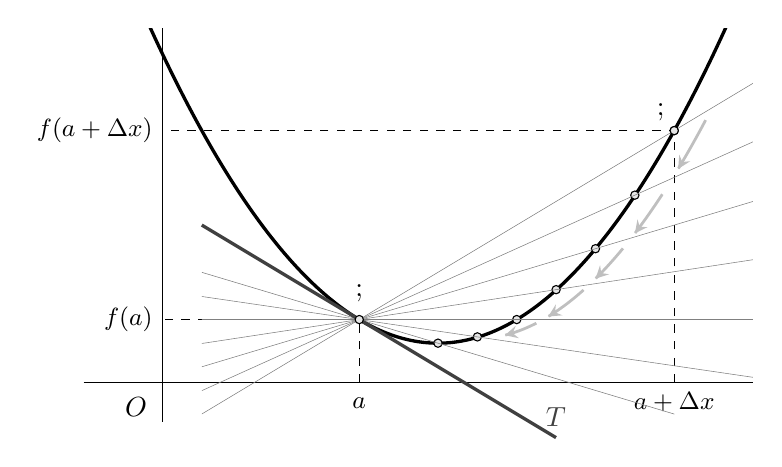
\begin{tikzpicture}[scale=1]
    
        \draw (-1,0) -- (7.5,0) (0,-.5) -- (0,4.5); % Axis
        \node[below left=2pt and 2pt] at (0,0) {$O$}; % Origin
        
        % Function curve        
        \begin{scope}       
            \clip (-1,0) rectangle (7.5,4.5);
            \draw[line width=1.2pt,smooth,samples=100,domain=-2.5:7.5] plot(\x,{0.3*((\x)-3.5)*((\x)-3.5)+0.5}); 
        \end{scope}
        
        \def\xA{2.5} \def\yA{0.8}
        \coordinate (A) at (\xA,\yA);
        \draw[dashed] (\xA,0) node[below=2pt] {\small $a$} -- (A) -- (0,\yA) node[left] {\small $f(a)$};
                
        \def\xM{6.5} \def\yM{3.2}
        \coordinate (M) at (\xM,\yM);
        \draw[dashed] (\xM,0) node[below] {\small $a+\Delta x$} -- (M) -- (0,\yM) node[left] {\small $f(a+\Delta x)$};
        \begin{scope}       
            \clip (0.5,-0.5) rectangle (7.5,4.5);

            % Series of lines all through point A
            \foreach \xN/\yN in {6.5/3.2,6/2.38,5.5/1.7,5/1.18,4.5/0.8,4/0.58,3.5/0.5}
                {
                \coordinate (N) at (\xN,\yN);
                \tkzDrawPoint[size=3](N)
                \tkzDrawLine[add=2 and 3,color=gray](A,N)
                }   
        \end{scope}
        
        \draw[line width=1.2pt,color=gray!50!black,smooth,samples=100,domain=0.5:5] plot(\x,{-0.6*(\x)+2.3}) node[above] {$T$};            
        
        \tkzDrawPoints[size=3](A,M);
        \tkzLabelPoint[above=3pt](A);
        \tkzLabelPoint[above left](M);
        
        %%%%Arrows alongside the curve
        \foreach \a/\b in {6.55/6.9, 6/6.35, 5.5/5.85, 4.9/5.35, 4.35/4.75}
            {
            \draw[<-,>=stealth,line width=1pt,color=gray!50!white,smooth,samples=100,domain=\a:\b] plot(\x,{0.32*((\x)-3.95)*((\x)-3.95)+0.55});
            }
        
    \end{tikzpicture}
\end{flushright}

\vspace{\stretch{1}}

Consider the function $y=\begin{cases}
                        x^2 & x\le0\\ 2x & x>0
                        \end{cases}$. What is the derivative of the function at $x=0$?
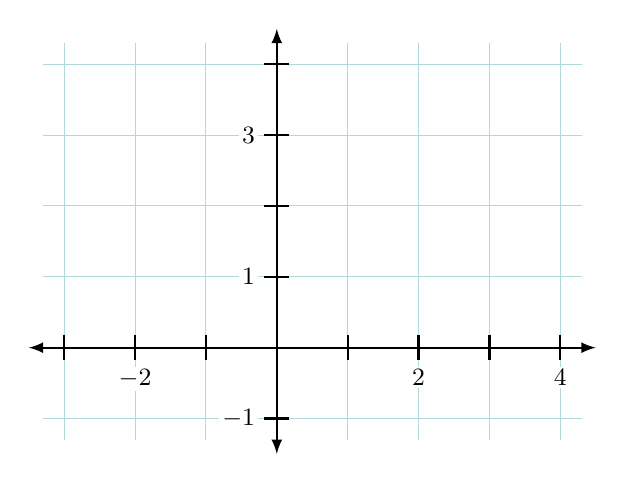
\begin{tikzpicture}[xscale=.9,yscale=.9]
    \draw[step=1,style=help lines,] (-3.3,-1.3) grid (4.3,4.3);
    \draw[latex-latex, thick] (-3.5,0)--(4.5,0);
    \draw[latex-latex, thick] (0,-1.5)--(0,4.5);
    \foreach \x in {-2,2,4}
        \draw[thick] (\x,5pt) -- (\x,-5pt) node [below=.7mm,fill=white,inner sep=1pt] {\small$\x$};
    \foreach \y in {-1,1,3}
        \draw[thick] (5pt,\y) -- (-5pt,\y) node [left=.7mm,fill=white,inner sep=1pt] {\small$\y$};
    \foreach \x in {-3,-1,1,3}
        \draw[thick] (\x,5pt) -- (\x,-5pt);
    \foreach \y in {2,4}
        \draw[thick] (5pt,\y) -- (-5pt,\y);
\end{tikzpicture}


\newpage

\noindent\textbf{Four Instances where a Derivative will Fail to Exist:}
\begin{questions}
    
    \begin{minipage}[t]{0.45\linewidth}
        \question At a \textbf{corner}, where the one-sided derivatives differ.\\
        \begin{center}
            Example: $f(x)=|x|$
            
            \vspace{2.5mm}
            
            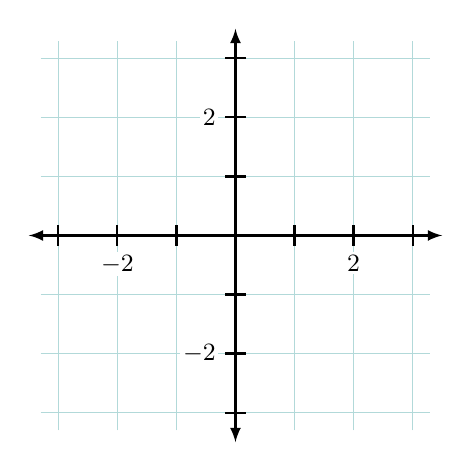
\begin{tikzpicture}[xscale=.75,yscale=.75]
                \draw[step=1,style=help lines,] (-3.3,-3.3) grid (3.3,3.3);
                \draw[latex-latex, thick] (-3.5,0)--(3.5,0);
                \draw[latex-latex, thick] (0,-3.5)--(0,3.5);
                \foreach \x in {-2,2}
                    \draw[thick] (\x,5pt) -- (\x,-5pt) node [below=.7mm,fill=white,inner sep=1pt] {\small$\x$};
                \foreach \y in {-2,2}
                    \draw[thick] (5pt,\y) -- (-5pt,\y) node [left=.7mm,fill=white,inner sep=1pt] {\small$\y$};
                \foreach \x in {-3,-1,1,3}
                    \draw[thick] (\x,5pt) -- (\x,-5pt);
                \foreach \y in {-1,1,-3,3}
                    \draw[thick] (5pt,\y) -- (-5pt,\y);
            \end{tikzpicture}
        \end{center}
    \end{minipage}
    \hfill
    \begin{minipage}[t]{0.45\linewidth}
        \question At a \textbf{cusp}, where the slopes of the secant lines approach $\infty$ from one side and $-\infty$ from the other. 
        \begin{center}
            Example: $f(x)=x^{2/3}$
            
            \vspace{2mm}
            
            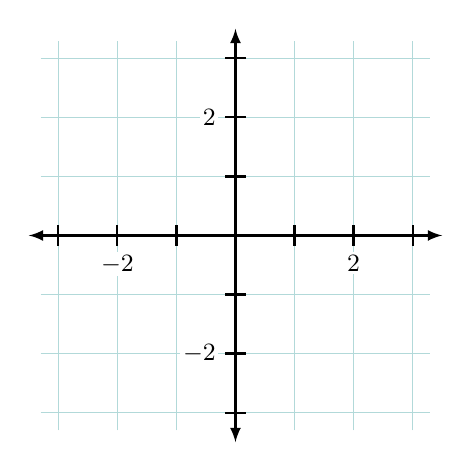
\begin{tikzpicture}[xscale=.75,yscale=.75]
                \draw[step=1,style=help lines,] (-3.3,-3.3) grid (3.3,3.3);
                \draw[latex-latex, thick] (-3.5,0)--(3.5,0);
                \draw[latex-latex, thick] (0,-3.5)--(0,3.5);
                \foreach \x in {-2,2}
                    \draw[thick] (\x,5pt) -- (\x,-5pt) node [below=.7mm,fill=white,inner sep=1pt] {\small$\x$};
                \foreach \y in {-2,2}
                    \draw[thick] (5pt,\y) -- (-5pt,\y) node [left=.7mm,fill=white,inner sep=1pt] {\small$\y$};
                \foreach \x in {-3,-1,1,3}
                    \draw[thick] (\x,5pt) -- (\x,-5pt);
                \foreach \y in {-1,1,-3,3}
                    \draw[thick] (5pt,\y) -- (-5pt,\y);
            \end{tikzpicture}
        \end{center}
    \end{minipage}
    
    
    \begin{minipage}[t]{0.45\linewidth}
        \question At a \textbf{vertical tangent}, where the slopes of the secant lines approach either $\infty$ or $-\infty$ from both sides.
        \begin{center}
            Example: $f(x)=\sqrt[3]{x}$
            
            \vspace{2.5mm}
            
            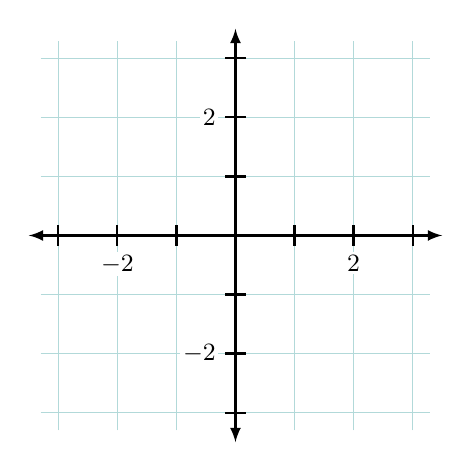
\begin{tikzpicture}[xscale=.75,yscale=.75]
                \draw[step=1,style=help lines,] (-3.3,-3.3) grid (3.3,3.3);
                \draw[latex-latex, thick] (-3.5,0)--(3.5,0);
                \draw[latex-latex, thick] (0,-3.5)--(0,3.5);
                \foreach \x in {-2,2}
                    \draw[thick] (\x,5pt) -- (\x,-5pt) node [below=.7mm,fill=white,inner sep=1pt] {\small$\x$};
                \foreach \y in {-2,2}
                    \draw[thick] (5pt,\y) -- (-5pt,\y) node [left=.7mm,fill=white,inner sep=1pt] {\small$\y$};
                \foreach \x in {-3,-1,1,3}
                    \draw[thick] (\x,5pt) -- (\x,-5pt);
                \foreach \y in {-1,1,-3,3}
                    \draw[thick] (5pt,\y) -- (-5pt,\y);
            \end{tikzpicture}
        \end{center}
    \end{minipage}
    \hfill
    \begin{minipage}[t]{0.45\linewidth}
        \question At a \textbf{point of discontinuity}.
        
        \vspace{3.3mm}
        
        \begin{center}
            Example: $f(x)=\begin{cases}
            -1 & x<0\\ 1 & x\ge0
            \end{cases}$
            
            \vspace{2mm}
            
            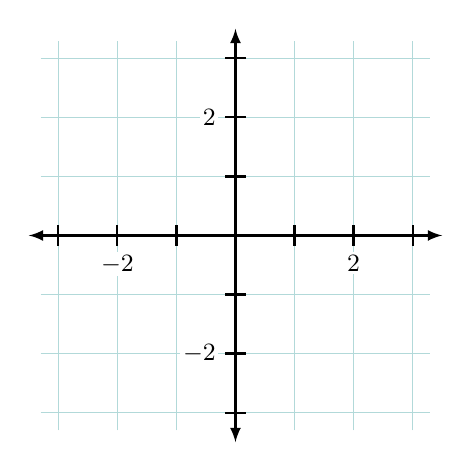
\begin{tikzpicture}[xscale=.75,yscale=.75]
                \draw[step=1,style=help lines,] (-3.3,-3.3) grid (3.3,3.3);
                \draw[latex-latex, thick] (-3.5,0)--(3.5,0);
                \draw[latex-latex, thick] (0,-3.5)--(0,3.5);
                \foreach \x in {-2,2}
                    \draw[thick] (\x,5pt) -- (\x,-5pt) node [below=.7mm,fill=white,inner sep=1pt] {\small$\x$};
                \foreach \y in {-2,2}
                    \draw[thick] (5pt,\y) -- (-5pt,\y) node [left=.7mm,fill=white,inner sep=1pt] {\small$\y$};
                \foreach \x in {-3,-1,1,3}
                    \draw[thick] (\x,5pt) -- (\x,-5pt);
                \foreach \y in {-1,1,-3,3}
                    \draw[thick] (5pt,\y) -- (-5pt,\y);
            \end{tikzpicture}
        \end{center}
    \end{minipage}

\end{questions}

\vfill

\begin{center}
    \begin{itemize}
        \item \textbf{A function must be continuous at \textit{a} to be differentiable at \textit{a}.}
        \item \textbf{If a function is continuous at \textit{a}, that does not mean that it is differentiable.}
        \item \textbf{If a function is differentiable at \textit{a}, then the function is continuous at \textit{a}.}
    \end{itemize}
\end{center}

\vfill

\newpage


The derivative at a point is the slope of the line tangent to the curve at that point. We use this fact to graph derivatives of functions.\\
\\
\noindent\textbf{Examples:}\\
Graph $\displaystyle f(x)=(x-2)^2+1$, then graph the derivative of the function.

\begin{minipage}[t]{0.45\linewidth}
    \begin{center}
        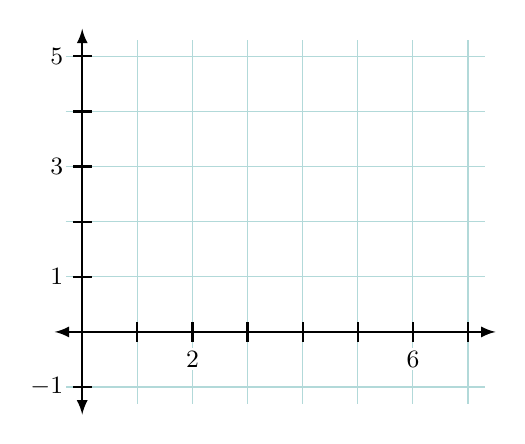
\begin{tikzpicture}[xscale=.7,yscale=.7]
            \draw[step=1,style=help lines,] (-0.3,-1.3) grid (7.3,5.3);
            \draw[latex-latex, thick] (-.5,0)--(7.5,0);
            \draw[latex-latex, thick] (0,-1.5)--(0,5.5);
            \foreach \x in {2,6}
                \draw[thick] (\x,5pt) -- (\x,-5pt) node [below=.7mm,fill=white,inner sep=1pt] {\small$\x$};
            \foreach \y in {-1,1,3,5}
                \draw[thick] (5pt,\y) -- (-5pt,\y) node [left=.7mm,fill=white,inner sep=1pt] {\small$\y$};
            \foreach \x in {1,3,4,5,7}
                \draw[thick] (\x,5pt) -- (\x,-5pt);
            \foreach \y in {2,4}
                \draw[thick] (5pt,\y) -- (-5pt,\y);
        \end{tikzpicture}
    \end{center}
\end{minipage}
\hfill
\begin{minipage}[t]{0.45\linewidth}
    \begin{center}
        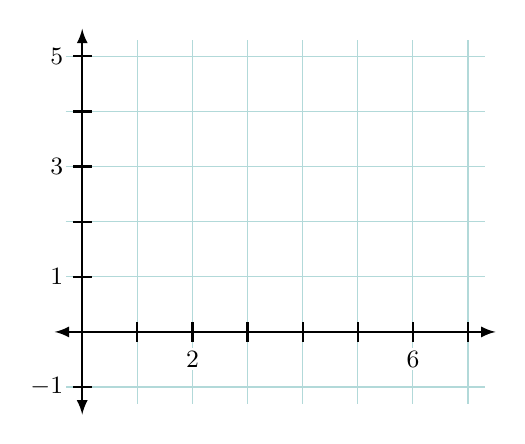
\begin{tikzpicture}[xscale=.7,yscale=.7]
            \draw[step=1,style=help lines,] (-0.3,-1.3) grid (7.3,5.3);
            \draw[latex-latex, thick] (-.5,0)--(7.5,0);
            \draw[latex-latex, thick] (0,-1.5)--(0,5.5);
            \foreach \x in {2,6}
                \draw[thick] (\x,5pt) -- (\x,-5pt) node [below=.7mm,fill=white,inner sep=1pt] {\small$\x$};
            \foreach \y in {-1,1,3,5}
                \draw[thick] (5pt,\y) -- (-5pt,\y) node [left=.7mm,fill=white,inner sep=1pt] {\small$\y$};
            \foreach \x in {1,3,4,5,7}
                \draw[thick] (\x,5pt) -- (\x,-5pt);
            \foreach \y in {2,4}
                \draw[thick] (5pt,\y) -- (-5pt,\y);
        \end{tikzpicture}
    \end{center}
\end{minipage}


Graph a positive cubic function passing through the point $(0,\,1)$ and having a maximum at $(2,\,4)$ and a minimum at $(6,\,1)$. Graph the derivative of the function.

\begin{minipage}[t]{0.45\linewidth}
    \begin{center}
        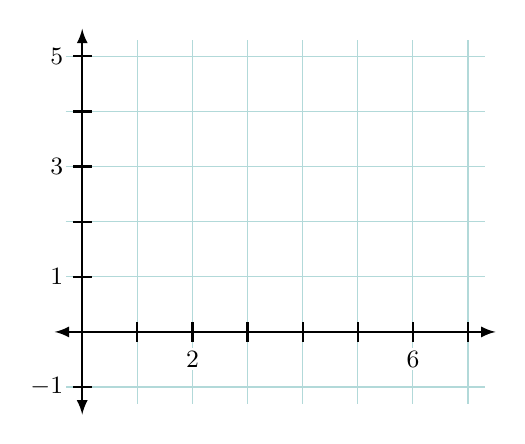
\begin{tikzpicture}[xscale=.7,yscale=.7]
            \draw[step=1,style=help lines,] (-0.3,-1.3) grid (7.3,5.3);
            \draw[latex-latex, thick] (-.5,0)--(7.5,0);
            \draw[latex-latex, thick] (0,-1.5)--(0,5.5);
            \foreach \x in {2,6}
                \draw[thick] (\x,5pt) -- (\x,-5pt) node [below=.7mm,fill=white,inner sep=1pt] {\small$\x$};
            \foreach \y in {-1,1,3,5}
                \draw[thick] (5pt,\y) -- (-5pt,\y) node [left=.7mm,fill=white,inner sep=1pt] {\small$\y$};
            \foreach \x in {1,3,4,5,7}
                \draw[thick] (\x,5pt) -- (\x,-5pt);
            \foreach \y in {2,4}
                \draw[thick] (5pt,\y) -- (-5pt,\y);
        \end{tikzpicture}
    \end{center}
\end{minipage}
\hfill
\begin{minipage}[t]{0.45\linewidth}
    \begin{center}
        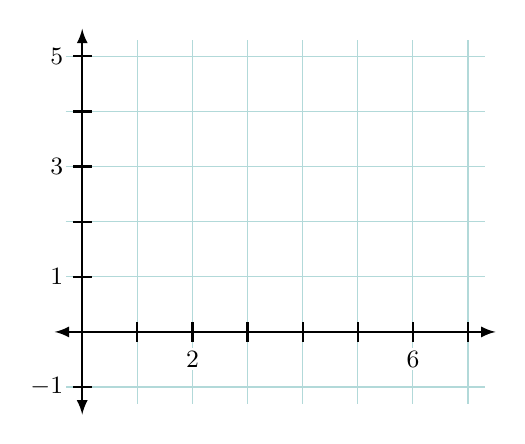
\begin{tikzpicture}[xscale=.7,yscale=.7]
            \draw[step=1,style=help lines,] (-0.3,-1.3) grid (7.3,5.3);
            \draw[latex-latex, thick] (-.5,0)--(7.5,0);
            \draw[latex-latex, thick] (0,-1.5)--(0,5.5);
            \foreach \x in {2,6}
                \draw[thick] (\x,5pt) -- (\x,-5pt) node [below=.7mm,fill=white,inner sep=1pt] {\small$\x$};
            \foreach \y in {-1,1,3,5}
                \draw[thick] (5pt,\y) -- (-5pt,\y) node [left=.7mm,fill=white,inner sep=1pt] {\small$\y$};
            \foreach \x in {1,3,4,5,7}
                \draw[thick] (\x,5pt) -- (\x,-5pt);
            \foreach \y in {2,4}
                \draw[thick] (5pt,\y) -- (-5pt,\y);
        \end{tikzpicture}
    \end{center}
\end{minipage}


Now let's try it backwards!!!  Graph $\displaystyle f'(x)=\begin{cases}
2 & x>1\\ -1 & x<1
\end{cases}$ below. Given that $f(0)=0$ and $f(x)$ is continuous, graph $f(x)$.

\begin{minipage}[t]{0.45\linewidth}
    \begin{center}
        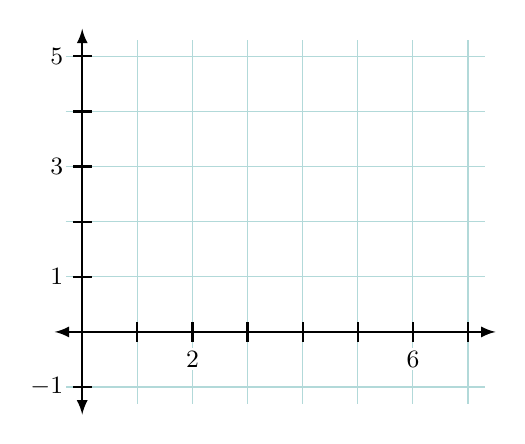
\begin{tikzpicture}[xscale=.7,yscale=.7]
            \draw[step=1,style=help lines,] (-0.3,-1.3) grid (7.3,5.3);
            \draw[latex-latex, thick] (-.5,0)--(7.5,0);
            \draw[latex-latex, thick] (0,-1.5)--(0,5.5);
            \foreach \x in {2,6}
                \draw[thick] (\x,5pt) -- (\x,-5pt) node [below=.7mm,fill=white,inner sep=1pt] {\small$\x$};
            \foreach \y in {-1,1,3,5}
                \draw[thick] (5pt,\y) -- (-5pt,\y) node [left=.7mm,fill=white,inner sep=1pt] {\small$\y$};
            \foreach \x in {1,3,4,5,7}
                \draw[thick] (\x,5pt) -- (\x,-5pt);
            \foreach \y in {2,4}
                \draw[thick] (5pt,\y) -- (-5pt,\y);
        \end{tikzpicture}
    \end{center}
\end{minipage}
\hfill
\begin{minipage}[t]{0.45\linewidth}
    \begin{center}
        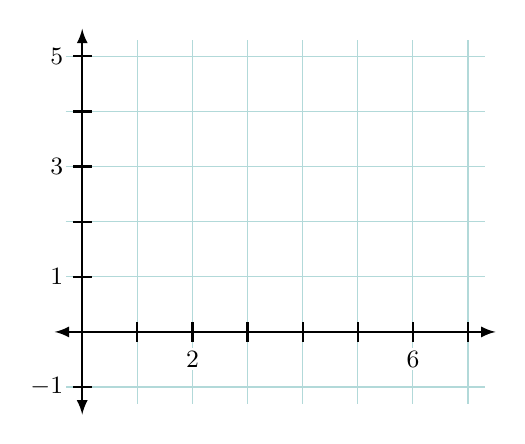
\begin{tikzpicture}[xscale=.7,yscale=.7]
            \draw[step=1,style=help lines,] (-0.3,-1.3) grid (7.3,5.3);
            \draw[latex-latex, thick] (-.5,0)--(7.5,0);
            \draw[latex-latex, thick] (0,-1.5)--(0,5.5);
            \foreach \x in {2,6}
                \draw[thick] (\x,5pt) -- (\x,-5pt) node [below=.7mm,fill=white,inner sep=1pt] {\small$\x$};
            \foreach \y in {-1,1,3,5}
                \draw[thick] (5pt,\y) -- (-5pt,\y) node [left=.7mm,fill=white,inner sep=1pt] {\small$\y$};
            \foreach \x in {1,3,4,5,7}
                \draw[thick] (\x,5pt) -- (\x,-5pt);
            \foreach \y in {2,4}
                \draw[thick] (5pt,\y) -- (-5pt,\y);
        \end{tikzpicture}
    \end{center}
\end{minipage}



\newpage
\phantomsection\addcontentsline{toc}{subsection}{Extreme Values of Functions}
\subsection*{Extreme Values of Functions}
Extreme values help us answer questions like, \textit{What is the most effective dose of medicine?}, \textit{What is the least expensive way to pipe oil from an offshore refinery down the coast?}\\
\\
\\

\textbf{Absolute} (or global) maximum and minimums means there is no greater/lesser value for $f(x)$ anywhere.\\
\\
\textbf{Local} maximum and minimum means there is no greater/lesser value for $f(x)$ nearby.\\
\\
\textbf{Domain Matters!} Given that $\displaystyle f(x)=\frac{1}{3}x^3-x^2$, find the absolute extrema and the local extrema on the following intervals:

\begin{minipage}[t]{.65\linewidth}
    \hspace{\stretch{8}} local max \hspace{\stretch{1}} abs max \hspace{\stretch{1}} local min \hspace{\stretch{1}} abs min\\
    
    \begin{questions}
        \question $\displaystyle(-\infty,\,\infty)$\\\\
        
        \question $\displaystyle[-3,\,6]$\\\\
        
        \question $\displaystyle(0,\,6]$\\\\
        
        \question $\displaystyle[-3,\,-1]$\\
    \end{questions}
\end{minipage}
\hfill
\begin{minipage}[t]{.25\linewidth}
    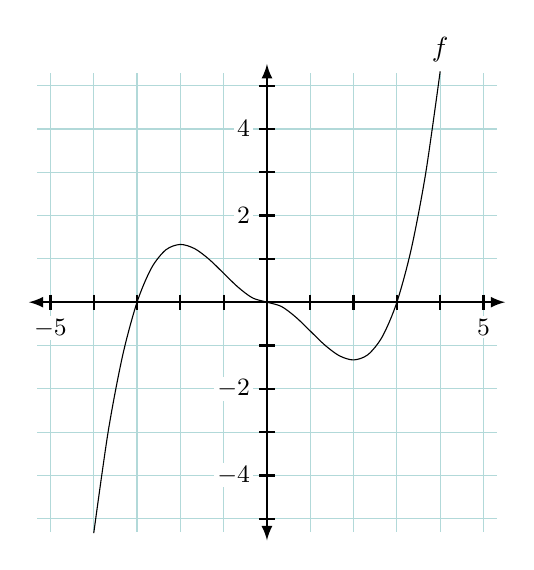
\begin{tikzpicture}[xscale=.55,yscale=.55,baseline=(current bounding box.north)]
        \draw[step=1,style=help lines,] (-5.3,-5.3) grid (5.3,5.3);
        \draw[latex-latex, thick] (-5.5,0)--(5.5,0);
        \draw[latex-latex, thick] (0,-5.5)--(0,5.5);
        \foreach \x in {-5,5}
            \draw[thick] (\x,5pt) -- (\x,-5pt) node [below=.7mm,fill=white,inner sep=1pt] {\small$\x$};
        \foreach \y in {-2,2,-4,4}
            \draw[thick] (5pt,\y) -- (-5pt,\y) node [left=.7mm,fill=white,inner sep=1pt] {\small$\y$};
        \foreach \x in {-3,-1,1,3,2,-2,4,-4}
            \draw[thick] (\x,5pt) -- (\x,-5pt);
        \foreach \y in {1,-1,3,-3,5,-5}
            \draw[thick] (5pt,\y) -- (-5pt,\y);
            
        \draw[] plot[smooth, domain=-4:4] (\x, {(1/3)*(\x^(3))-(\x^(2))}) node[anchor=south] {$f$};
    \end{tikzpicture}
    
\end{minipage}
\vspace{1cm}

\begin{tcolorbox}[title= THE EXTREME VALUE THEOREM,colframe=black,sharp corners,colback=white,colbacktitle=white,coltitle=black,boxrule=1pt]

    If $f(x)$ is continuous on the closed interval $[a,\,b]$, then $f(x)$ has both a maximum value and a minimum value on the interval.
    
\end{tcolorbox}
\vspace{1cm}
Naturally the question becomes: \textbf{How can we find the extreme values?} \underline{\hspace{3cm}}!!!!


\newpage


\begin{tcolorbox}[title= DEFINITION OF LOCAL EXTREME VALUES,colframe=black,sharp corners,colback=white,colbacktitle=white,coltitle=black,boxrule=1pt]

    If a function $f(x)$ has a local maximum or minimum value at an interior point $c$ of its domain, and if $f'(x)$ exists at $c$, then $f'(c)=0$. 
    
\end{tcolorbox}
\vspace{1cm}
But sometimes a maximum or a minimum may occur when $f'(c)\ne0$. What might cause this to happen?
\begin{center}
    \underline{\hspace{6cm}}
\end{center}
\vspace{2cm}

Instead, lets introduce a definition that encompasses ALL these points:\\

\begin{tcolorbox}[title= DEFINITION OF A CRITICAL POINT,colframe=black,sharp corners,colback=white,colbacktitle=white,coltitle=black,boxrule=1pt]

    Let $f$ be defined at $c$. If $f'(c)=0$ or if $f$ is not differentiable at $c$, then $c$ is a \textbf{critical point} (or \textbf{critical number}) of $f$.\\
    \\
    As a consequence, \textbf{relative extrema only occur at critical points!}
    
\end{tcolorbox}
\vspace{.15cm}
\noindent\textbf{Example:}\\
Find the extrema of $f(x)=3x^4-4x^3$ on the interval $[1,\,2]$.

\newpage

\noindent\textbf{More Examples:}
\begin{questions}
    \question Find the absolute maximum and minimum values of $f(x)=x^{2/3}$ on the interval $[-2,\,3]$.
    \vspace{\stretch{1}}
    
    \question Find the extreme values of  $\displaystyle f(x)=\frac{1}{\sqrt{4-x^2}}$.
    \vspace{\stretch{1}}
    
    \question Find the extreme values of $\displaystyle f(x)=\begin{cases}
    5-2x^2 & x\le1\\ x+2 & x>1
    \end{cases}$.
    \vspace{\stretch{1}}
    
    \question Find the extreme values of $\displaystyle f(x)=\ln\left|\frac{x}{1+x^2}\right|$.
    \vspace{\stretch{1}}
    
    \question Let $f(x)=|x^3-9x|$
        \begin{parts}
            \part Does $f'(0)$ exist?
            \part Does $f'(3)$ exist?
            \part Does $f'(-3)$ exist?
            \part Determine all extrema of $f(x)$.
        \end{parts}
\end{questions}

\newpage

\begin{tcolorbox}[title= THE FIRST DERIVATIVE TEST,colframe=black,sharp corners,colback=white,colbacktitle=white,coltitle=black,boxrule=1pt]

    The following applies to a continuous function $f(x)$.
    \begin{questions}
        \question If $f'(x)$ changes sign from positive to negative at a critical point $c$, then $f(x)$ has a local maximum value at $c$.
        \question If $f'(x)$ changes sign from negative to positive at a critical point $c$, then $f(x)$ has a local minimum value at $c$.
        \question If $f'(x)$ does not change sign at a critical point $c$, then $f(x)$ has no local extreme value at $c$.
    \end{questions}
    
    
\end{tcolorbox}
\vspace{.15cm}
\textbf{Examples:} Identify any local extrema using the first derivative test. Then identify any absolute extrema.
\begin{questions}
    \begin{minipage}{.45\linewidth}
        \question $\displaystyle f(x)=x^2-12x-5$
    \end{minipage}
    \hfill
    \begin{minipage}{.45\linewidth}
        \question $\displaystyle g(x)=\left(x^2-3\right)e^x$
    \end{minipage}
\end{questions}

\vspace{\stretch{1}}

There are times when a curve can hold water or spill water. We call this ability \textbf{concavity}.\\

\begin{tcolorbox}[title= THE CONCAVITY TEST,colframe=black,sharp corners,colback=white,colbacktitle=white,coltitle=black,boxrule=1pt]
    The graph of a twice differentiable function $f(x)$ is
    \begin{questions}
        \question concave up if $f''(x)>0$.
        \question concave down if $f''(x)<0$.
    \end{questions}
    
    The point where the graph has a tangent line and when the concavity changes is a \textbf{point of inflection}. When $f''(x)=0$ or $f''(x)$ DNE are both candidates for POI's.
    
\end{tcolorbox}


\newpage


\begin{tcolorbox}[title= THE SECOND DERIVATIVE TEST,colframe=black,sharp corners,colback=white,colbacktitle=white,coltitle=black,boxrule=1pt]

    \begin{questions}
        \question If $f'(c)=0$ and $f''(c)<0$, then $f(x)$ has a local maximum at $x=c$.
        \question If $f'(c)=0$ and $f''(c)>0$, then $f(x)$ has a local minimum at $x=c$.
    \end{questions}
    
    The test fails if $f''(c)=0$ or if $f''(c)$ does not exist.
    
\end{tcolorbox}

\textbf{Examples:} Find the local extreme values of the following.
\begin{questions}
    \begin{minipage}{.45\linewidth}
        \question $y=x^4$
    \end{minipage}
    \hfill
    \begin{minipage}{.45\linewidth}
        \question $f(x)=\sqrt[3]{x}$
    \end{minipage}

    \vspace{\stretch{1}}
\end{questions}

\phantomsection\addcontentsline{toc}{subsection}{Curve Sketching}
\subsection*{Curve Sketching}

\begin{tcolorbox}[colframe=black,sharp corners,colback=white,boxrule=.25mm]
    \begin{center}
        \textbf{Summary for Graphing Functions}
    \end{center}
    
    \vspace{.7cm}
    
    \begin{questions}
        \question Use pre-calculus and algebra
        \begin{parts}
            \part know the general shape
            \part find the $y$-intercept $(x=0)$
            \part find the roots/zeros $(y=0)$
            \part determine the vertical asymptotes (denom=0) and limits
            \part determine the horizontal or slant asymptotes
            \part use limits $x\to\pm\infty$ to determine end behavior
        \end{parts}
        
        \question Use the first derivative
        \begin{parts}
            \part determine the critical points
            \part make a first derivative sign chart to see where function is increasing or decreasing
            \part apply first derivative test to determine extrema
        \end{parts}
        
        \question Use the second derivative
        \begin{parts}
            \part determine possible points of inflection
            \part apply the second derivative test to determine extrema
            \part make a sign chart to determine concavity
        \end{parts}
    \end{questions}
    
\end{tcolorbox}

\newpage
\begin{minipage}[t]{.65\linewidth}
    \begin{center}
        \textbf{Example 1:} $y=x^3-3x^2+4$
    \end{center}
    
    \vspace{.3cm}
    
    \begin{questions}
        \question The first derivative is
        \vspace{.15cm}
        
        \question The second derivative is
        \vspace{.15cm}
        
        \question The function is increasing on
        \vspace{.15cm}
        
        \question The function is decreasing on
        \vspace{.15cm}
        
        \question The function is concave up on
        \vspace{.15cm}
        
        \question The function is concave down on
        \vspace{.15cm}
        
        \question The absolute maximum is
        \vspace{.15cm}
        
        \question The absolute minimum is
        \vspace{.15cm}
        
        \question The local maximum(s) is(are)
        \vspace{.15cm}
        
        \question The local minimums(s) is(are)
        \vspace{.15cm}
        
        \question The point(s) of inflection is(are)
    \end{questions}
\end{minipage}
\hfill
\begin{minipage}[t]{.25\linewidth}
    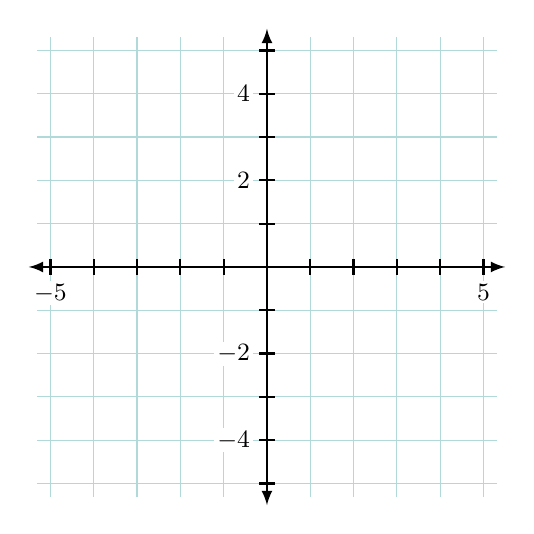
\begin{tikzpicture}[xscale=.55,yscale=.55,baseline=(current bounding box.north)]
        \draw[step=1,style=help lines,] (-5.3,-5.3) grid (5.3,5.3);
        \draw[latex-latex, thick] (-5.5,0)--(5.5,0);
        \draw[latex-latex, thick] (0,-5.5)--(0,5.5);
        \foreach \x in {-5,5}
            \draw[thick] (\x,5pt) -- (\x,-5pt) node [below=.7mm,fill=white,inner sep=1pt] {\small$\x$};
        \foreach \y in {-2,2,-4,4}
            \draw[thick] (5pt,\y) -- (-5pt,\y) node [left=.7mm,fill=white,inner sep=1pt] {\small$\y$};
        \foreach \x in {-3,-1,1,3,2,-2,4,-4}
            \draw[thick] (\x,5pt) -- (\x,-5pt);
        \foreach \y in {1,-1,3,-3,5,-5}
            \draw[thick] (5pt,\y) -- (-5pt,\y);
    \end{tikzpicture}
    
\end{minipage}

\vspace{\stretch{1}}


\begin{minipage}[t]{.65\linewidth}
    \begin{center}
        \textbf{Example 2:} $\displaystyle y=\frac{5}{2x-4}$
    \end{center}
    
    \vspace{.3cm}
    
    \begin{questions}
        \question The first derivative is
        \vspace{.15cm}
        
        \question The second derivative is
        \vspace{.15cm}
        
        \question The function is increasing on
        \vspace{.15cm}
        
        \question The function is decreasing on
        \vspace{.15cm}
        
        \question The function is concave up on
        \vspace{.15cm}
        
        \question The function is concave down on
        \vspace{.15cm}
        
        \question The absolute maximum is
        \vspace{.15cm}
        
        \question The absolute minimum is
        \vspace{.15cm}
        
        \question The local maximum(s) is(are)
        \vspace{.15cm}
        
        \question The local minimums(s) is(are)
        \vspace{.15cm}
        
        \question The point(s) of inflection is(are)
    \end{questions}
\end{minipage}
\hfill
\begin{minipage}[t]{.25\linewidth}
    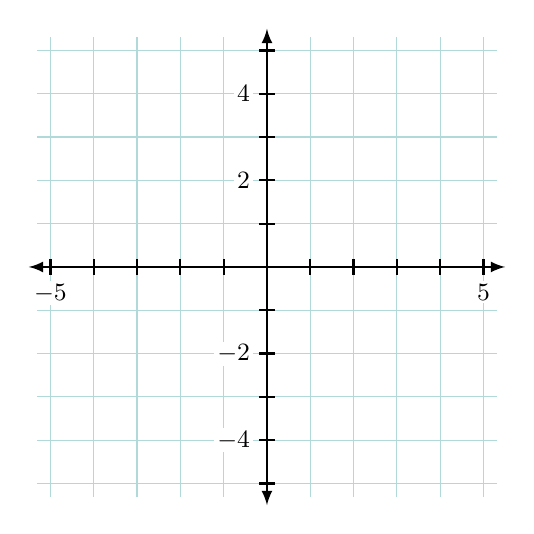
\begin{tikzpicture}[xscale=.55,yscale=.55,baseline=(current bounding box.north)]
        \draw[step=1,style=help lines,] (-5.3,-5.3) grid (5.3,5.3);
        \draw[latex-latex, thick] (-5.5,0)--(5.5,0);
        \draw[latex-latex, thick] (0,-5.5)--(0,5.5);
        \foreach \x in {-5,5}
            \draw[thick] (\x,5pt) -- (\x,-5pt) node [below=.7mm,fill=white,inner sep=1pt] {\small$\x$};
        \foreach \y in {-2,2,-4,4}
            \draw[thick] (5pt,\y) -- (-5pt,\y) node [left=.7mm,fill=white,inner sep=1pt] {\small$\y$};
        \foreach \x in {-3,-1,1,3,2,-2,4,-4}
            \draw[thick] (\x,5pt) -- (\x,-5pt);
        \foreach \y in {1,-1,3,-3,5,-5}
            \draw[thick] (5pt,\y) -- (-5pt,\y);
    \end{tikzpicture}
    
\end{minipage}

\vspace{\stretch{1}}

\newpage

\begin{minipage}[t]{.65\linewidth}
    \begin{center}
        \textbf{Example 3:} $\displaystyle y=\frac{x^2}{x^2-1}$
    \end{center}
    
    \vspace{.3cm}
    
    \begin{questions}
        \question The first derivative is
        \vspace{.15cm}
        
        \question The second derivative is
        \vspace{.15cm}
        
        \question The function is increasing on
        \vspace{.15cm}
        
        \question The function is decreasing on
        \vspace{.15cm}
        
        \question The function is concave up on
        \vspace{.15cm}
        
        \question The function is concave down on
        \vspace{.15cm}
        
        \question The absolute maximum is
        \vspace{.15cm}
        
        \question The absolute minimum is
        \vspace{.15cm}
        
        \question The local maximum(s) is(are)
        \vspace{.15cm}
        
        \question The local minimums(s) is(are)
        \vspace{.15cm}
        
        \question The point(s) of inflection is(are)
    \end{questions}
\end{minipage}
\hfill
\begin{minipage}[t]{.25\linewidth}
    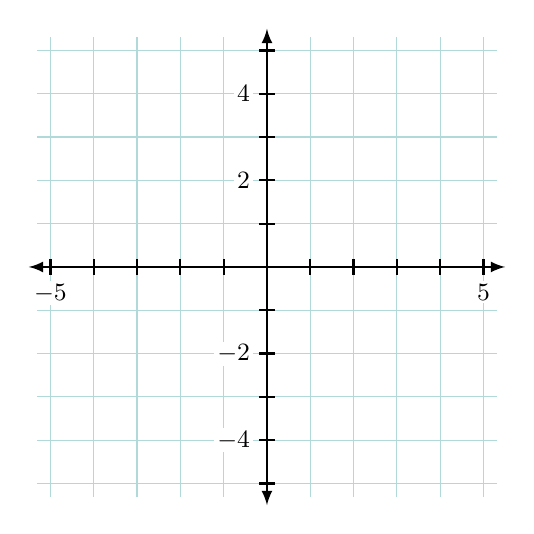
\begin{tikzpicture}[xscale=.55,yscale=.55,baseline=(current bounding box.north)]
        \draw[step=1,style=help lines,] (-5.3,-5.3) grid (5.3,5.3);
        \draw[latex-latex, thick] (-5.5,0)--(5.5,0);
        \draw[latex-latex, thick] (0,-5.5)--(0,5.5);
        \foreach \x in {-5,5}
            \draw[thick] (\x,5pt) -- (\x,-5pt) node [below=.7mm,fill=white,inner sep=1pt] {\small$\x$};
        \foreach \y in {-2,2,-4,4}
            \draw[thick] (5pt,\y) -- (-5pt,\y) node [left=.7mm,fill=white,inner sep=1pt] {\small$\y$};
        \foreach \x in {-3,-1,1,3,2,-2,4,-4}
            \draw[thick] (\x,5pt) -- (\x,-5pt);
        \foreach \y in {1,-1,3,-3,5,-5}
            \draw[thick] (5pt,\y) -- (-5pt,\y);
    \end{tikzpicture}
    
\end{minipage}

\vspace{\stretch{1}}


\begin{minipage}[t]{.65\linewidth}
    \begin{center}
        \textbf{Example 4:} $\displaystyle y=\frac{x^2+x-2}{x-2}$
    \end{center}
    
    \vspace{.3cm}
    
    \begin{questions}
        \question The first derivative is
        \vspace{.15cm}
        
        \question The second derivative is
        \vspace{.15cm}
        
        \question The function is increasing on
        \vspace{.15cm}
        
        \question The function is decreasing on
        \vspace{.15cm}
        
        \question The function is concave up on
        \vspace{.15cm}
        
        \question The function is concave down on
        \vspace{.15cm}
        
        \question The absolute maximum is
        \vspace{.15cm}
        
        \question The absolute minimum is
        \vspace{.15cm}
        
        \question The local maximum(s) is(are)
        \vspace{.15cm}
        
        \question The local minimums(s) is(are)
        \vspace{.15cm}
        
        \question The point(s) of inflection is(are)
    \end{questions}
\end{minipage}
\hfill
\begin{minipage}[t]{.25\linewidth}
    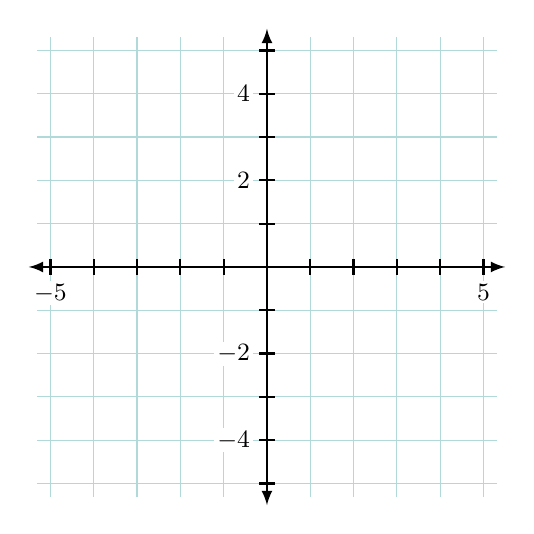
\begin{tikzpicture}[xscale=.55,yscale=.55,baseline=(current bounding box.north)]
        \draw[step=1,style=help lines,] (-5.3,-5.3) grid (5.3,5.3);
        \draw[latex-latex, thick] (-5.5,0)--(5.5,0);
        \draw[latex-latex, thick] (0,-5.5)--(0,5.5);
        \foreach \x in {-5,5}
            \draw[thick] (\x,5pt) -- (\x,-5pt) node [below=.7mm,fill=white,inner sep=1pt] {\small$\x$};
        \foreach \y in {-2,2,-4,4}
            \draw[thick] (5pt,\y) -- (-5pt,\y) node [left=.7mm,fill=white,inner sep=1pt] {\small$\y$};
        \foreach \x in {-3,-1,1,3,2,-2,4,-4}
            \draw[thick] (\x,5pt) -- (\x,-5pt);
        \foreach \y in {1,-1,3,-3,5,-5}
            \draw[thick] (5pt,\y) -- (-5pt,\y);
    \end{tikzpicture}
    
\end{minipage}

\vspace{\stretch{1}}


\newpage
\phantomsection\addcontentsline{toc}{subsection}{Mean Value Theorem}
\subsection*{Mean Value Theorem \textit{\tiny (for derivatives)}}

\begin{tcolorbox}[title= THE MEAN VALUE THEOREM,colframe=black,sharp corners,colback=white,colbacktitle=white,coltitle=black,boxrule=1pt]

    If $f$ is continuous on the closed interval $[a,\,b]$ and differentiable in the open interval $(a,\,b)$, then there exists a number $c$ in $(a,\,b)$ such that
    \[f'(c)=\frac{f(b)-f(a)}{b-a}.\]
    
\end{tcolorbox}
\vspace{2cm}

\textit{Think about it graphically:}
\vspace{2cm}

Another example: if a car accelerating from 0 takes 8 seconds to go 352 ft, its average velocity for the 8 second interval is 44 ft/sec (30 mph). At some point during the acceleration, the speedometer \textit{must} read exactly 30 mph!\\
\\
\textbf{Examples:} For each of the following functions on the indicated intervals, determine whether or not the MVT applies. If it does, find the value(s) where the mean value is attained.
\begin{questions}
    \question $\displaystyle f(x)=x^3+1$ on $[1,\,2]$
    \vspace{\stretch{1}}
    
    \question $\displaystyle f(x)=\sqrt{x^2}+1$ on $[-1,\,1]$
    \vspace{\stretch{1}}
    
    \question $\displaystyle f(x)=\frac{3}{x+2}$ on $[-3,\,1]$
    \vspace{\stretch{1}}
    
    \question $\displaystyle f(x)=\begin{cases}
    x^3+3 & x<1\\ x^2+1 & x\ge1
    \end{cases}$ on $[-2,\,2]$
    \vspace{\stretch{1}}
\end{questions}



\newpage
\phantomsection\addcontentsline{toc}{subsection}{Modeling \& Optimization}
\subsection*{Modeling \& Optimization}
\begin{questions}
    \question An open-top box is to be made by cutting congruent squares of side length x from the corners of a 20-by-25-inch sheet of tin and bending up the sides.  Find how large the cut-out squares should be so that the box can hold as much as possible.  Find the resulting maximum volume. [1, 7]
    
    \vspace{\stretch{2}}
    
    \question Find the largest possible value of $2x+y$  if x and y are the lengths of the sides of a right triangle whose hypotenuse is $\sqrt{5}$ units long. [2]
    
    \vspace{\stretch{1}}
    
    \newpage
    
    \question Find two positive numbers whose sum is 36 and whose product is as large as possible. [3, 6]
    \vspace{\stretch{1}}

    \question The city recreation department plans to build a rectangular playground having an area of 3600 square meters and surround it by a fence.  Find the dimensions of the rectangle that uses the least amount of fencing.  [4, 8, 11, 16]
    \vspace{\stretch{1}}

    \question Find the radius and height of a right circular cylinder that minimizes total surface area for a volume of $36\pi$ cubic inches.  [5, 9]
    \vspace{\stretch{1}}
    
    \newpage
    
    \question An isosceles triangle has its vertex at the origin and its base parallel to the x-axis with the vertices above the axis on the curve $y=27-x^2$. Find the largest area the triangle can have. [10, 19]
    \vspace{\stretch{1}}
    
    \question A carpenter has been asked to build an open box with a square base.  The sides of the box will cost \$3 per square meter, and the base will cost \$4 per square meter.  Find the dimensions of the box of greatest volume that can be constructed for \$48.  [12,13,14,17]
    \vspace{\stretch{1}}
    
    \question Find the dimensions of the right circular cylinder of greatest volume inscribed in a right circular cone of radius 10 inches and a height of 24 inches.  [15, 18]
    \vspace{\stretch{1}}
    
    
\end{questions}




\newpage
\phantomsection\addcontentsline{toc}{subsection}{Related Rates}
\subsection*{Related Rates}
\begin{questions}
    \question A snowball is melting at a rate of 2 cubic feet per hour.  If it remains spherical, at what rate is the radius changing when the radius of the snowball is 20 inches?  At what rate is the surface area changing when the radius is 20 inches?  [1, 2, 3]
    \vspace{\stretch{1.7}}
    
    \question A small funnel in the shape of a cone is being emptied of fluid at the rate of 12 cubic centimeters per second.  The height of the funnel is 20 centimeters and the radius of the top is 4 centimeters.  How fast is the fluid level dropping when the level stands 5 centimeters above the vertex?  [4, 5]
    \vspace{\stretch{1}}
    
    \newpage
    
    \question Sand is poured on a conical pile at a rate of 20 cubic meters per minute.  The height of the pile is always equal to the radius of the base of the pile.  When the pile is 3 meters high, how fast is the height of the pile increasing?  [6]
    \vspace{\stretch{1}}
    
    You can now complete [14, 16, 18, 20, 22, 24, and 25]
    \question A ladder leans against a vertical wall with the bottom of the ladder 8 feet from the wall on a horizontal floor.  At that time, the bottom end of the ladder is being pulled away at the rate of 3 ft/sec and the top of the ladder slips down the wall at the rate of 4 ft/sec.  How long is the ladder?  [7, 8, 9, 10, 15, 17, 19, 21, 23]
    \vspace{\stretch{1}}
    
    \question An object moves on a parabola $3y=x^2$. When $x = 3$, the $x$-coordinate of the object is increasing at the rate of 1 foot per minute.  How fast is the $y$-coordinate increasing at that moment?  [11, 12]
    \vspace{\stretch{1}}
    
    \newpage
    
    \question A balloon rises vertically at the rate of 5 ft/sec.  A person on the ground 200 feet away from the spot below the rising balloon watches the balloon ascend.  At what rate is the distance between the balloon and the observer changing when the balloon is 50 feet above the ground? \textbf{Don’t confuse this problem with the following one!}
    
    \vspace{\stretch{1}}
    
    \question A balloon rises vertically at the rate of 10 feet per second.  A person watches the balloon ascend from a point on the ground that is 100 feet away from the spot below the rising balloon.  At what rate (radian/second) is the observer’s head rotating upward to follow the balloon when the balloon is 50 feet above the level of the observer’s head?  [13]
    \vspace{\stretch{1}}
    
    \question A man 6 feet tall walks at a rate of 5 ft/sec toward a street light that is 16 feet above the ground.  At what rate is the tip of his shadow moving?  At what rate is the length of his shadow changing when he is 10 feet from the base of the light? [26, 27]
    
    \vspace{\stretch{1}}
    
    
\end{questions}






\newpage
\phantomsection\addcontentsline{toc}{subsection}{L'Hopital's Rule}
\subsection*{L'Hopital's Rule}
Remember when we computed $\displaystyle\lim_{x\to0}\frac{\sin x}{x}$? We got $\frac{0}{0}$, which is called an \textbf{indeterminate form}. While we could use Squeeze Theorem to show that this limit becomes 1, it would be easier to show using \textbf{L'Hopital's Rule}.

\begin{tcolorbox}[title= L'HOPITAL'S RULE,colframe=black,sharp corners,colback=white,colbacktitle=white,coltitle=black,boxrule=1pt]

    Suppose that $f(a)=g(a)=0$, that $f'(a)$ and $g'(a)$ exist, and that $g'(x)\ne0$. Then
    \[\lim_{x\to a}\frac{f(a)}{g(a)}=\frac{f'(a)}{g'(a)}\]
    
\end{tcolorbox}

\begin{center}
    \textbf{\large DO NOT USE QUOTIENT RULE!}
\end{center}
\noindent\textbf{Examples:}
\begin{questions}
    \question $\displaystyle \lim_{x\to0}\frac{3x-\sin x}{x}$
    \vspace{\stretch{1}}
    
    \question $\displaystyle \lim_{x\to0}\frac{\sqrt{x+1}-1}{x}$
    \vspace{\stretch{1}}
    
    \question $\displaystyle \lim_{x\to0}\frac{\sqrt{x+1}-1-x/2}{x-2}$
    \vspace{\stretch{1}}
    
    \question $\displaystyle \lim_{x\to\pi/2}\frac{1+\sec x}{\tan x}$
    \vspace{\stretch{1}}
\end{questions}



%%make linearization and newton's method take-home packets

\newpage
\phantomsection\addcontentsline{toc}{subsection}{Differentials, Linearization, Newton's Method}
\subsection*{Differentials}
\begin{tcolorbox}[title= DEFINITION OF A DIFFERENTIAL,colframe=black,sharp corners,colback=white,colbacktitle=white,coltitle=black,boxrule=1pt]

    Let $y=f(x)$ be a differentiable function. The differential $dx$ is an independent variable. The differential $dy$ is $dy=f'(x)\,dx$.
    
\end{tcolorbox}
\noindent\textbf{Examples:} Find the differential $dy$ and evaluate $dy$ for the given values of $x$ and $dx$.
\begin{questions}
    \question $y=x^5+37x,\,x=1,\,dx=0.01$
    \vspace{\stretch{.8}}
    
    \question $y=\sin3x,\,x=\pi,\,dx=-0.02$
    \vspace{\stretch{.8}}
    
    \question $x+y=xy,\,x=2,\,dx=0.05$
    \vspace{\stretch{.8}}
\end{questions}

We can use differentials to estimate the change in the value of a function! Let $f(x)$ be differentiable at $x=a$. The approximate change in the value of $f(x)$ when $x$ changes from $a$ to $a+dx$ is $df=f'(a)\,dx$.
\begin{questions}
    \setcounter{question}{3}
    \question The radius of a circle is to be increased from $r=10$ to $r=10.1$. Use differentials to estimate the change in area. Calculate the estimated percent change.
    \vspace{\stretch{1.2}}
\end{questions}

\subsection*{Linearization \& Newton's Method}
This section has been replaced with a small take-home assignment. Expect to see this material on a quiz of test. It is not dense enough to merit the use of in-class instruction. Come find me outside of class if you have questions.

\begin{center}
    Link to File:
    
    \vspace{.2cm}
    
    \qrcode{https://drive.google.com/file/d/1GqxwEAv6EcMuU0GQZDaL8cGVEBIjYr5e/view?usp=sharing}
    
\end{center}



\newpage
\phantomsection\addcontentsline{toc}{section}{Integrals}
\phantomsection\addcontentsline{toc}{subsection}{Basic Integration Rules}
\subsection*{Basic Integration Rules}
Given $dy/dx$, find $y$.
\begin{questions}
    \begin{minipage}{0.45\linewidth}
        \question $\displaystyle\frac{dy}{dx}=6x$
    \end{minipage}
    \hfill
    \begin{minipage}{0.45\linewidth}
        \question $\displaystyle\frac{dy}{dx}=4x^3+2$
    \end{minipage}
    
    \vspace{\stretch{1}}
\end{questions}
Are you \textit{sure}?


\begin{tcolorbox}[title= DEFINITION OF THE INDEFINITE INTEGRAL,colframe=black,sharp corners,colback=white,colbacktitle=white,coltitle=black,boxrule=1pt]

    The indefinite integral of $f$ with respect to $x$ is the set of all antiderivatives of a function $f(x)$.
    \[\int f(x)\,dx=F(x)+C\]
    
\end{tcolorbox}

\begin{center}
    We use the following general formula for polynomials:
    \[\int x^n\,dx=\frac{x^{n+1}}{n+1}+C,\,n\ne1\]
\end{center}

\noindent\textbf{Examples:}
\begin{questions}
    \question $\displaystyle\int6x\,dx$
    \vspace{\stretch{1}}
    
    \question $\displaystyle\int(4x^3+2)\,dx$
    \vspace{\stretch{1}}
    
    \question $\displaystyle\int-dx$
    \vspace{\stretch{1}}
    
    \question $\displaystyle\int\frac{x^5+3x-2}{x^3}\,dx$
    \vspace{\stretch{1}}
    
    \newpage
    
    \question $\displaystyle\int\left(7\sqrt[3]{x^4}+x\right)\,dx$
    \vspace{\stretch{1}}
\end{questions}

How would you approach integrating $\displaystyle\int 4x^3\left(x^4-1\right)\,dx$?
\vspace{\stretch{1}}

You would distribute and then do each term individually. However, there are going to be integrals where that method is not going to be preferred. Therefore, I will softly introduce a new method called \textbf{Integration by Substitution}.

\noindent\textbf{Examples:} Evaluate the following integrals.
\begin{questions}
    \question $\displaystyle\int15x^2(5x^3-2)^4\,dx$
    \vspace{\stretch{1}}
    
    \question $\displaystyle\int x^2\sqrt{5+2x^3}\,dx$
    \vspace{\stretch{1}}
    
    Solve the Differential Equation
    \question $\displaystyle\frac{dy}{dx}=3x^2\sqrt{1+x^3},$ given that $y=1$ when $x=0$.
    \vspace{\stretch{1}}
\end{questions}



\newpage
\phantomsection\addcontentsline{toc}{subsection}{Integration of Trigonometric Functions}
\subsection*{Integration of Trigonometric Functions}
Before we begin, let's check out the list of basic trig integrals that you should have memorized (these are just derivatives in reverse, so nothing new here).

\begin{tcolorbox}[title= INTEGRALS OF BASIC TRIG FUNCTIONS,colframe=black,sharp corners,colback=white,colbacktitle=white,coltitle=black,boxrule=1pt]

    \begin{align*}
        \int\sin x\,dx &= -\cos x+C & \int\csc^2 x\,dx &= -\cot x+C\\
        \int\cos x\,dx &= \sin x+C & \int\sec x\tan x\,dx &= \sec x+C\\
        \int\sec^2 x\,dx &= \tan x+C & \int\csc x\cot x\,dx &= -\csc x+C
    \end{align*}
    \vspace{.05cm}
\end{tcolorbox}
Also... you are going to need to know a lot of trig identities.

\noindent\textbf{Examples:} Where possible, try rewriting using trig identities before integrating.
\begin{questions}
    \question $\displaystyle\int\frac{1}{\cos^2 x}\,dx$
    \vspace{\stretch{1}}
    
    \question $\displaystyle\int\frac{\sin x}{\tan x}\,dx$
    \vspace{\stretch{1}}
    
    
    The following examples require \textbf{Integration by Substitution}. The key to doing these problems is learning when the angle should be chosen as $u$ or when to let the entire trig function be $u$.
    
    \begin{minipage}{0.45\linewidth}
        \question $\displaystyle\int\cos(2x)\,dx$    
    \end{minipage}
    \hfill
    \begin{minipage}{0.45\linewidth}
        \question $\displaystyle\int\frac{\sin x}{\cos^2 x}\,dx$
    \end{minipage}
    
    \vspace{\stretch{1.2}}
    
    \newpage
    
    \question $\displaystyle\int 16x\sin^3\left(2x^2+1\right)\cos\left(2x^2+1\right) \,dx$
    \vspace{\stretch{1}}
\end{questions}

\begin{tcolorbox}[title= INTEGRAL OF SECANT AND COSECANT,colframe=black,sharp corners,colback=white,colbacktitle=white,coltitle=black,boxrule=1pt]

    \[\displaystyle\int\sec u\,du=\ln|\sec u+\tan u|+C \hspace{.6in}\int\csc u\,du=-\ln|\csc u + \cot u|+C\]
    
\end{tcolorbox}
You \textbf{have} to memorize these. The algebraic trick to do the integration by hand is more annoying to remember than just having this formula ingrained in your memory.

\begin{questions}
    \question $\displaystyle \int 7x\sec(x^2)\,dx$
    
    \vspace{\stretch{1}}
    
    \question $\displaystyle \int \frac{\cos x+\sin x}{\tan x}\,dx$
    
    \vspace{\stretch{1}}
\end{questions}




\newpage
\phantomsection\addcontentsline{toc}{subsection}{Integration of Transcendental Functions}
\subsection*{Integration of Transcendental Functions}
\begin{tcolorbox}[title= INTEGRAL OF \textit{U}$^{-1}$,colframe=black,sharp corners,colback=white,colbacktitle=white,coltitle=black,boxrule=1pt]

    \[\displaystyle\int\frac{du}{u}=\ln|u|+C\]
    
\end{tcolorbox}

\noindent\textbf{Examples:}
\begin{questions}
    \begin{minipage}{0.45\linewidth}
        \question $\displaystyle\int\frac{2}{x}\,dx$
    \end{minipage}
    \hfill
    \begin{minipage}{0.45\linewidth}
        \question $\displaystyle\int\frac{\sec^2(2x)}{1+\tan(2x)}\,dx$
    \end{minipage}
    
    \vspace{\stretch{1}}
    
    \begin{minipage}{0.45\linewidth}
        \question $\displaystyle\int\frac{2}{2-3x}\,dx$
    \end{minipage}
    \hfill
    \begin{minipage}{0.45\linewidth}
        \question $\displaystyle\int\tan x\,dx$
    \end{minipage}
    
    \vspace{\stretch{1}}
    
\end{questions}

\begin{tcolorbox}[title= INTEGRAL OF EXPONENTIAL FUNCTIONS,colframe=black,sharp corners,colback=white,colbacktitle=white,coltitle=black,boxrule=1pt]

    \begin{align*}
        \displaystyle\int e^u\,du &= e^u +C & \displaystyle\int a^u\,du &= \displaystyle\frac{a^u}{\ln a}+C
    \end{align*}
    
\end{tcolorbox}

\noindent\textbf{Examples:}
\begin{questions}
    \begin{minipage}{0.45\linewidth}
        \question $\displaystyle\int x e^{x^2}\,dx$
    \end{minipage}
    \hfill
    \begin{minipage}{0.45\linewidth}
        \question $\displaystyle\int\frac{1}{e^x}\,dx$
    \end{minipage}
    
    \vspace{\stretch{1}}
    
    \begin{minipage}{0.45\linewidth}
        \question $\displaystyle\int5^x\,dx$
    \end{minipage}
    \hfill
    \begin{minipage}{0.45\linewidth}
        \question $\displaystyle\int\frac{e^{\sqrt{x}}}{\sqrt{x}}\,dx$
    \end{minipage}
    
    \vspace{\stretch{1}}
    
\end{questions}


\newpage

\begin{tcolorbox}[title= INTEGRALS OF INVERSE TRIG FUNCTIONS,colframe=black,sharp corners,colback=white,colbacktitle=white,coltitle=black,boxrule=1pt]

    \begin{align*}
        \displaystyle\int\frac{du}{\sqrt{a^2-u^2}} &= \arcsin\frac{u}{a}+C & \displaystyle\int\frac{du}{a^2+u^2} &= \displaystyle\frac{1}{a}\arctan\frac{u}{a}+C 
    \end{align*}
    \begin{align*}
        \displaystyle\int\frac{du}{u\sqrt{u^2-a^2}} &= \frac{1}{a}\text{arcsec}\frac{|u|}{a} +C
    \end{align*}
\end{tcolorbox}
\textbf{Examples:}
\begin{questions}
    \question $\displaystyle\int\frac{9}{2x^2+1}\,dx$
    \vspace{\stretch{1}}
    
    \question $\displaystyle\int\frac{-1}{3x\sqrt{9x^2-25}}\,dx$
    \vspace{\stretch{1}}
    
    
    \question $\displaystyle\int\frac{\cos\theta}{\sqrt{1-\sin^2\theta}}\,d\theta$
    \vspace{\stretch{1}}
\end{questions}


\newpage
\phantomsection\addcontentsline{toc}{subsection}{Constant of Integration \& Applications}
\subsection*{Finding the Constant of Integration}

\begin{questions}
    \question Given $f'(x)=4x^5$ and $f(1)=1$, find $f(x)$.
    \vspace{\stretch{1}}
    
    \question Given $f'(x)=(x^2-3x+2)(x-2)$ and $f(-2)=0$, find $f(x)$.
    \vspace{\stretch{1}}
    
    Solve the differential equations subject to the given initial conditions.
    \question $\displaystyle\frac{dy}{dx}=4(x-7)^3,\,y=10$ when $x=8$.
    \vspace{\stretch{1}}
    
    \question The graph of $y$ passes through the point $(4,\,13)$ with slope 5 and $\displaystyle\frac{d^2y}{dx^2}=\frac{3x}{8}$. Find $y$.
    \vspace{\stretch{1}}
\end{questions}

\subsection*{Applications of Integration}
\begin{questions}
    \setcounter{question}{4}
    \question A particle moving on a straight line has acceleration $a(t)=5-3t$ in ft/sec$^2$, and its velocity is 7 ft/sec at 2 seconds. If $s(t)$ is the distance from the origin, find $s(2)-s(1)$.
    
    \vspace{\stretch{.7}}
    
    \newpage
    
    \question A motorist applies the brakes on a car moving at 45 miles per hour on a straight road, and the brakes cause a constant deceleration of 22 ft/sec$^2$. In how many seconds will the car stop, and how many feet will the car have traveled after the time the brakes were applied?
    \vspace{\stretch{1}}
    
    \question Find the equation of a curve such that $y''$ is always 2, and at the point $(2,\,6)$ the slope of the tangent line is 10.
    \vspace{\stretch{1}}
    
    \question A stone is thrown straight up from a building ledge that is 120 feet above the ground with an initial velocity of 96 ft/sec. When will the stone reach its maximum height? What will the maximum height be? When will the stone hit the ground? With what speed will it hit the ground?
    \vspace{\stretch{1}}
    
    
\end{questions}


\newpage
\phantomsection\addcontentsline{toc}{subsection}{Definite Integration}
\subsection*{Definite Integration}
\begin{tcolorbox}[title= THE DEFINITE INTEGRAL,colframe=black,sharp corners,colback=white,colbacktitle=white,coltitle=black,boxrule=1pt]

    \[\displaystyle\int_a^b f(x\,dx)=F(x)|_a^b=F(b)-F(a)\]
    
\end{tcolorbox}
\noindent\textbf{Examples:} Compute the following.
\begin{questions}
    
    \question $\displaystyle\int_{0}^{\pi}\sin x\,dx$
    \vspace{\stretch{1}}
    
    \question $\displaystyle\int_{-2}^{1}\left(x^2+1\right)^2 \,dx$
    \vspace{\stretch{1}}
    
    \question $\displaystyle\int_{1}^{2}\left(3-\frac{6}{x^2}\right) \,dx$
    \vspace{\stretch{1}}
    
    \question $\displaystyle\int_{0}^{\pi} \sin^2 \theta\,d\theta$
    \vspace{\stretch{1}}
    
    \question $\displaystyle\int_{-1}^{0} x\sqrt{1-x^2}\,dx$
    \vspace{\stretch{1}}
    
\end{questions}

\newpage

\textbf{Changing the Limits of Integration}\\
Be careful that you do not write down the limits of integration when your integral is in terms of $u$ unless you change the limits of integration.\\
\\
\noindent\textbf{Examples:}

\begin{questions}
    
    \question $\displaystyle\int_{-1}^{0}\frac{x^3}{\sqrt{x^4+9}}\,dx$
    \vspace{\stretch{1}}
    
    \question $\displaystyle\int_{-\sqrt{3}}^{\sqrt{3}}\frac{4x}{\sqrt{x^2+1}} \,dx$
    \vspace{\stretch{1}}
    
    \question $\displaystyle\int_{\pi/6}^{\pi/3} (1-\cos3x)\sin3x \,dx$   
    \vspace{\stretch{1}}
    
\end{questions}




\newpage
\phantomsection\addcontentsline{toc}{subsection}{Area Under the Curve with RAM}
\subsection*{Area Under the Curve with RAM}
A train moves along a track at a steady rate of 75 miles per hour from 7 am to 9 am. What is the total distance traveled by the train? What if the train doesn't travel at a steady rate? Then how do you find the distance?
\vspace{\stretch{.6}}

Our goal is to calculate the area under a curve. We do that by breaking the area (which we cannot calculate) into rectangles (whose area we can calculate) and adding them together.

\begin{questions}
    
    \question Given $y=x^2$, what is the area under the curve from $x=0$ to $x=4$?
    
    \begin{minipage}[t]{0.3\linewidth}
        \begin{center}
        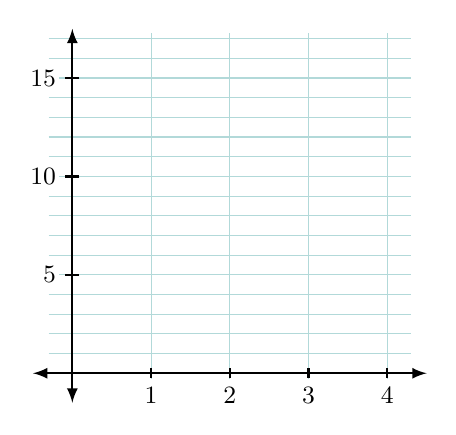
\begin{tikzpicture}[xscale=1,yscale=.25]
            \draw[step=1,style=help lines,] (-0.3,-.3) grid (4.3,17.3);
            \draw[latex-latex, thick] (-.5,0)--(4.5,0);
            \draw[latex-latex, thick] (0,-1.5)--(0,17.5);
            \foreach \x in {1,2,3,4}
                \draw[thick] (\x,7.5pt) -- (\x,-7.5pt) node [below=.7mm,fill=white,inner sep=1pt] {\small$\x$};
            \foreach \y in {5,10,15}
                \draw[thick] (2.5pt,\y) -- (-2.5pt,\y) node [left=.7mm,fill=white,inner sep=1pt] {\small$\y$};
        \end{tikzpicture}
        \end{center}
    \end{minipage}
    \hfill
    \begin{minipage}[t]{0.3\linewidth}
        \begin{center}
        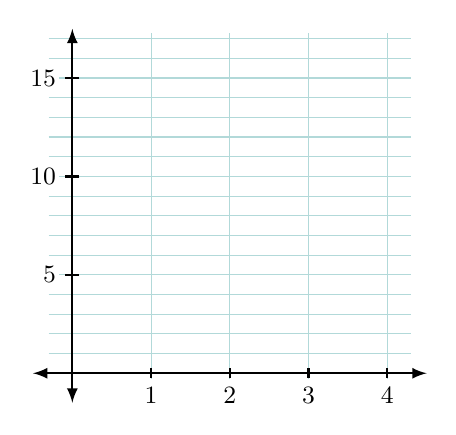
\begin{tikzpicture}[xscale=1,yscale=.25]
            \draw[step=1,style=help lines,] (-0.3,-.3) grid (4.3,17.3);
            \draw[latex-latex, thick] (-.5,0)--(4.5,0);
            \draw[latex-latex, thick] (0,-1.5)--(0,17.5);
            \foreach \x in {1,2,3,4}
                \draw[thick] (\x,7.5pt) -- (\x,-7.5pt) node [below=.7mm,fill=white,inner sep=1pt] {\small$\x$};
            \foreach \y in {5,10,15}
                \draw[thick] (2.5pt,\y) -- (-2.5pt,\y) node [left=.7mm,fill=white,inner sep=1pt] {\small$\y$};
        \end{tikzpicture}
        \end{center}
    \end{minipage}
    \hfill
    \begin{minipage}[t]{0.3\linewidth}
        \begin{center}
        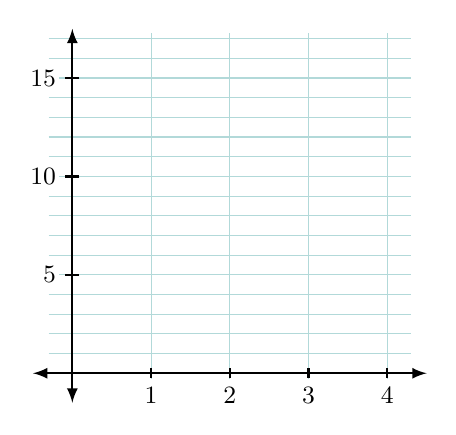
\begin{tikzpicture}[xscale=1,yscale=.25]
            \draw[step=1,style=help lines,] (-0.3,-.3) grid (4.3,17.3);
            \draw[latex-latex, thick] (-.5,0)--(4.5,0);
            \draw[latex-latex, thick] (0,-1.5)--(0,17.5);
            \foreach \x in {1,2,3,4}
                \draw[thick] (\x,7.5pt) -- (\x,-7.5pt) node [below=.7mm,fill=white,inner sep=1pt] {\small$\x$};
            \foreach \y in {5,10,15}
                \draw[thick] (2.5pt,\y) -- (-2.5pt,\y) node [left=.7mm,fill=white,inner sep=1pt] {\small$\y$};
        \end{tikzpicture}
        \end{center}
    \end{minipage}
    
    \vspace{\stretch{1}}
    
    \begin{center}
        \underline{RAM is the Rectangular Approximation Method}\\
        LRAM is the left hand values of $y$\\
        RRAM is the right hand values of $y$\\
        MRAM is the midpoint of L and R
    \end{center}
    
    \vspace{\stretch{.1}}
    
    \newpage
    
    \question Find the area between the $x$-axis and the curve $y=-x^2+2x+24$ using MRAM and 5 intervals (5 rectangles). MAKE A SKETCH along with your approximation.
    \vspace{\stretch{1}}
    
    
    \begin{minipage}[t]{0.55\linewidth}
    \question The table to the right shows the velocity of a model train engine moving along a track for 10 seconds. Estimate the distance traveled by the engine, using MRAM over 5 subintervals. Again, make a sketch!    
    \end{minipage}
    \hfill
    \begin{minipage}[t]{0.4\linewidth}
    \begin{longtable}[ht]{|C{2.25cm}|C{3cm}|}
        \hline
        Time (sec)\Tstrut\Bstrut & Velocity (in/sec)\Tstrut\Bstrut \\\hline
        $0$\Tstrut\Bstrut & $0$\Tstrut\Bstrut \\\hline
        $1$\Tstrut\Bstrut & $12$\Tstrut\Bstrut \\\hline
        $2$\Tstrut\Bstrut & $22$\Tstrut\Bstrut \\\hline
        $3$\Tstrut\Bstrut & $10$\Tstrut\Bstrut \\\hline
        $4$\Tstrut\Bstrut & $5$\Tstrut\Bstrut \\\hline 
        $5$\Tstrut\Bstrut & $13$\Tstrut\Bstrut \\\hline
        $6$\Tstrut\Bstrut & $11$\Tstrut\Bstrut \\\hline
        $7$\Tstrut\Bstrut & $6$\Tstrut\Bstrut \\\hline
        $8$\Tstrut\Bstrut & $2$\Tstrut\Bstrut \\\hline
        $9$\Tstrut\Bstrut & $6$\Tstrut\Bstrut \\\hline
        $10$\Tstrut\Bstrut & $0$\Tstrut\Bstrut \\\hline
    \end{longtable}    
    \end{minipage}
    

    
    
    \vspace{\stretch{.5}}
    
    \newpage
    
    \question Oil is leaking out of a tanker damaged at sea. The damage to the tanker is worsening as evidenced by the increased leakage each hour, recorded in the table below.
    \begin{parts}
        \part Give an upper and lower estimate of the total quantity of oil that has escaped over the 8 hours.
        \part The tanker continues to leak 720 gal/h after the first 8 hours. If the tanker originally contained 25,000 gallons of oil, approximately how many more hours will elapse in the worst case before all the oil has leaked? In the best case?
    \end{parts}
    
    
    \begin{longtable}[r]{|C{2cm}|C{3cm}|}
        \hline
        Time (h)\Tstrut\Bstrut & Leakage (gal/h)\Tstrut\Bstrut \\\hline
        $0$\Tstrut\Bstrut & $50$\Tstrut\Bstrut \\\hline
        $1$\Tstrut\Bstrut & $70$\Tstrut\Bstrut \\\hline
        $2$\Tstrut\Bstrut & $97$\Tstrut\Bstrut \\\hline
        $3$\Tstrut\Bstrut & $136$\Tstrut\Bstrut \\\hline
        $4$\Tstrut\Bstrut & $190$\Tstrut\Bstrut \\\hline 
        $5$\Tstrut\Bstrut & $265$\Tstrut\Bstrut \\\hline
        $6$\Tstrut\Bstrut & $369$\Tstrut\Bstrut \\\hline
        $7$\Tstrut\Bstrut & $516$\Tstrut\Bstrut \\\hline
        $8$\Tstrut\Bstrut & $720$\Tstrut\Bstrut \\\hline
    \end{longtable}    
    
    
    \hfill
    
    \vspace{\stretch{1}}
    
    \hfill
    
    \begin{longtable}[ht]{|C{1cm}|C{1cm}|C{1cm}|C{1cm}|C{1cm}|C{1cm}|}
        \hline
        $x$\Tstrut\Bstrut & $1$\Tstrut\Bstrut & $1.1$\Tstrut\Bstrut & $1.2$\Tstrut\Bstrut & $1.3$\Tstrut\Bstrut & $1.4$\Tstrut\Bstrut \\\hline
        $f'(x)$\Tstrut\Bstrut & $8$\Tstrut\Bstrut & $10$\Tstrut\Bstrut & $12$\Tstrut\Bstrut & $13$\Tstrut\Bstrut & $14.5$\Tstrut\Bstrut \\\hline
    \end{longtable}
    
    
    \question Use a Midpoint Riemann sum with two subintervals of equal length and values (directly above) from the table to approximate $\displaystyle\int_1^{1.4} f'(x)\,dx$.
    
    
    
\end{questions}


\newpage



\subsection*{Trapezoidal Rule}
\begin{tcolorbox}[title= THE TRAPEZOIDAL RULE, colframe=black,sharp corners,colback=white,colbacktitle=white,coltitle=black,boxrule=1pt]

    To approximate $\displaystyle\int_a^b f(x)\,dx$, use $\displaystyle T=\frac{h}{2}\left(y_0+2y_1+2y_2+2y_3+\dots+2y_{n-1}+y_n\right)$,
    where $[a,\,b]$ is partitioned into $n$ subintervals of equal length $\displaystyle h=\frac{b-a}{n}$.
    
\end{tcolorbox}

Fun Fact: $\displaystyle T=\frac{\text{LRAM}_n+\text{RRAM}_n}{2}$. However, this is not the same as MRAM!\\
\begin{questions}
    \question An observer measures the outside temperature sporadically from noon until midnight, recording the temperatures in the following table. What is the average temperature for the 12-hour period?
    
    \begin{longtable}{|C{.9cm}|C{.9cm}|C{.5cm}|C{.5cm}|C{.5cm}|C{.5cm}|C{.5cm}|C{.5cm}|C{.5cm}|C{1.4cm}|}
        \hline
        Time \Tstrut\Bstrut & Noon \Tstrut\Bstrut & 1 \Tstrut\Bstrut & 2 \Tstrut\Bstrut & 4 \Tstrut\Bstrut & 5 \Tstrut\Bstrut & 8 \Tstrut\Bstrut & 9 \Tstrut\Bstrut & 10\Tstrut\Bstrut & Mdnt \Tstrut\Bstrut \\\hline
        Temp \Tstrut\Bstrut & 63\Tstrut\Bstrut & 65\Tstrut\Bstrut & 66\Tstrut\Bstrut & 70\Tstrut\Bstrut & 69\Tstrut\Bstrut & 65\Tstrut\Bstrut & 64\Tstrut\Bstrut & 62\Tstrut\Bstrut & 55\Tstrut\Bstrut \\\hline
    \end{longtable}  
    
    
\end{questions}

\vspace{\stretch{1.5}}

\subsection*{Riemann Approximations}
Basically, all the rectangle approximations \textit{are} Riemann approximations (or "Riemann Sums"). While this is a separate section in most textbooks, let this be another word that equates to a process you already know.



\newpage
\phantomsection\addcontentsline{toc}{subsection}{The Definite Integral as Area Under the Curve}
\subsection*{The Definite Integral as Area Under the Curve}

\begin{center}
\begin{tikzpicture}[xscale=1.3,yscale=.65,declare function={f(\x)=((1/3)*(\x)^(3)-3*(\x)^(2)+8*\x-3;}]
\coordinate (start) at (.8,{f(.8)});
\coordinate (x0) at (1,{f(1)});
\coordinate (x1) at (2,{f(2)});
\coordinate (x2) at (3,{f(3)});
\coordinate (x3) at (4,{f(4)});
\coordinate (x4) at (5,{f(5)});
\coordinate (end) at (5.05,{f(5.05)});

\draw [-latex] (-0.5,0) -- (6,0) node (xaxis) [below] {$x$};
\draw [-latex] (0,-0.5) -- (0,5) node [left] {$y$};
\foreach \x/\xtext in {1/a , 5/b }
 \draw[xshift=\x cm] (0pt,3pt) -- (0pt,0pt) 
node[below=2pt,fill=white,font=\normalsize]
  {$\xtext$};
\draw[domain=.5:5.3,samples=200,variable=\x,<->,thick] plot ({\x},{f(\x)}); \end{tikzpicture}
\end{center}

The area under the curve can be estimated using $\displaystyle S_n=\sum_{k=1}^n f\left(c_k\right)\cdot\Delta x_k$, a Riemann sum for $f$ on the interval $[a,\,b].$

\begin{tcolorbox}[title= LIMIT DEFINITION OF THE DEFINITE INTEGRAL,colframe=black,sharp corners,colback=white,colbacktitle=white,coltitle=black,boxrule=1pt]

     Let $f$ be continuous on $[a,\,b]$, and let $[a,\,b]$ be partitioned into $n$ subintervals of equal length $\displaystyle \Delta x=\frac{b-a}{n}$. Then the definite integral of $f$ over $[a,\,b]$ is given by
     \[\lim_{n\to\infty}\sum_{k=1}^n f\left(c_k\right)\Delta x,\]
     where each $c_k$ is chosen arbitrarily in the $k^{\text{th}}$ subinterval.
    
\end{tcolorbox}

\noindent\textbf{Think!} Interpret the above definition and translate into less "mathy" talk:
\vspace{\stretch{.6}}

%actually build out this section and add more examples/explanations/etc.

\textbf{Using the Notation}\\
The interval $[-1,\,3]$ is partitioned into $n$ subintervals of equal length $\Delta x=4/n$. Let $m_k$ denote the midpoint of the $k^{\text{th}}$ subinterval. Express the limit $\displaystyle\lim_{n\to\infty}\sum_{k=1}^n \left( 3\left(m_l\right)^2-2m_k +5 \right)\Delta x$ as an integral.
\vspace{\stretch{.5}}

\newpage

\phantomsection\addcontentsline{toc}{subsection}{Limit-to-Integral and Integral-to-Limit}
\subsection*{Limit to Integral and Integral to Limit}
This section is to be completed after finishing Unit 5: Sequences and Series. The skills required to be fluent in this section will be strengthened in that unit immensely. In my personal opinion, it would be too many unrelated skills to be able to master amongst all the other content this unit holds.

There will be a standalone assessment on this topic at some point after the conclusion of Unit 5. The module involving this topic will be unlocked but not expected to be completed for quite some time.

\begin{center}
    \hspace{0pt}
    \vfill
    \textbf{Link to Notes}
    \vspace{.7cm}
    
    \qrcode{https://drive.google.com/file/d/1NBu7JxlZUY0V1fztLIygu6aRVqlerBnX/view?usp=sharing}    
    \vfill
    \hspace{0pt}
\end{center}

\newpage

\begin{tcolorbox}[title= DEFINITION OF THE DEFINITE INTEGRAL,colframe=black,sharp corners,colback=white,colbacktitle=white,coltitle=black,boxrule=1pt]

     \textbf{Formal:} If $y=f(x)$ is nonnegative and integrable over a closed interval $[a,\,b]$, then the area under the curve of $y=f(x)$ from $a$ to $b$ is the integral of $f$ from $a$ to $b$,
     \[A=\int_a^b f(x)\,dx\]
     
     \textbf{Informal:} The integral is the NET area between the curve and the $x$-axis. Parts of the area above the curve are positive and parts below the curve are negative.
    
\end{tcolorbox}

\begin{questions}
    \question Evaluate $\displaystyle\int_0^{5\pi/2}\sin x\,dx$.
    \vspace{\stretch{1}}
    
    For the following, evaluate the definite integral and find the TOTAL area between the curve and the $x$-axis.
    \question $\displaystyle\int_2^{\pi+2}\sin(x-2)\,dx$
    \vspace{\stretch{1}}
    
    \question Evaluate the integral $\displaystyle\int_{-2}^{2}\sqrt{4-x^2}\,dx$ using your calculator and confirm graphically that this is the area between the curve and the $x$-axis.
    \vspace{\stretch{1}}
    
    This even works for constant functions! Remember the train problem from the other day? A train moves along a track at a steady rate of 75 miles per hour from 7 am to 9 am. Express the total distance traveled as an integral. Evaluate the integral.
\end{questions}



\newpage
\phantomsection\addcontentsline{toc}{subsection}{Average Value \& Mean Value Theorem}
\subsection*{AVT \& MVT}
\begin{tcolorbox}[title= AVERAGE VALUE OF A FUNCTION,colframe=black,sharp corners,colback=white,colbacktitle=white,coltitle=black,boxrule=1pt]

     If $f$ is integrable on $[a,\,b]$, its average (mean) value on $[a,\,b]$ is
     \[\text{ave}(f)=\frac{1}{b-a}\int_a^b f(x)\,dx.\]
    
\end{tcolorbox}
\begin{questions}
    \question Find the average value of $f(x)=3x^2-2x$ on $[1,\,4]$.
    \vspace{\stretch{1}}
\end{questions}

\begin{tcolorbox}[title= THE MEAN VALUE THEOREM FOR DEFINITE INTEGRALS,colframe=black,sharp corners,colback=white,colbacktitle=white,coltitle=black,boxrule=1pt]

     If $f$ is continuous on $[a,\,b]$, then at some point $c$ in $[a,\,b]$,
     \[f(c)=\frac{1}{b-a}\int_a^b f(x)\,dx.\]
    
\end{tcolorbox}
\begin{questions}
    \setcounter{question}{1}
    \question Suppose we have a circle of radius $r$ centered at the origin. What is the average length of the chords perpendicular to the diameter $[-r,\,r]$ on the $x$-axis?
    \vspace{\stretch{1}}
\end{questions}

\newpage


\begin{center}
    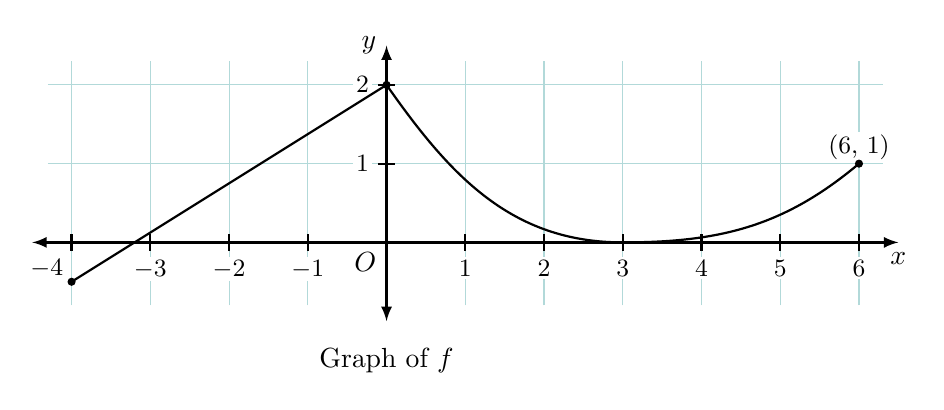
\begin{tikzpicture}[xscale=1,yscale=1,baseline=(current bounding box.north)]
        \draw[step=1,style=help lines,] (-4.3,-.8) grid (6.3,2.3);
        \draw[latex-latex, thick] (-4.5,0)-- (0,0) node [below left] {$O$}-- (6.5,0) node[below] {$x$};
        \draw[latex-latex, thick] (0,-1)--(0,2.5) node[left] {$y$};
        \foreach \x in {-3,-2,-1,1,2,3,4,5,6}
            \draw[thick] (\x,3pt) -- (\x,-3pt) node [below=.7mm,fill=white,inner sep=1pt] {\small$\x$};
        \draw[thick] (-4,3pt) -- (-4,-3pt) node [below left=.82mm,fill=white,inner sep=1pt] {\small$-4$};
        \foreach \y in {1,2}
            \draw[thick] (3pt,\y) -- (-3pt,\y) node [left=.7mm,fill=white,inner sep=1pt] {\small$\y$};
        
        \draw[-,thick] (-4,-.5) -- (0,2);
        \filldraw (-4,-.5) circle (1.25pt);
        \filldraw (0,2) circle (1.25pt);
        
        \draw[-,thick] (0,2) to [out=-55,in=180] (3,0);
        \draw[-,thick] (3,0) to[out=0,in=-140] (6,1) node [above,fill=white,inner sep=1pt] {\small$(6,\,1)$};
        \filldraw (6,1) circle (1.25pt);
        
        \node at (0,-1.5) {Graph of $f$};
        
    \end{tikzpicture}
\end{center}

\begin{questions}
    \setcounter{question}{2}
    \question A continuous function $f$ is defined on the closed interval $[-4,\,6]$. The graph of $f$ consists of a line segments and a curve that is tangent to the $x-$axis at $x=3$, as shown in the figure above. On the interval $0<x<6$, the function $f$ is twice differentiable, with $f''(x)>0$.\\
    \\
    Is there a value of $a$, with $-4\le a<6$, for which the Mean Value Theorem, applied on the interval $[a,\,6]$, guarantees a value $c$, with $a<c<6$, at which $f'(c)=\frac{1}{3}$? Justify your answer.
\end{questions}


\newpage
\phantomsection\addcontentsline{toc}{subsection}{The Fundamental Theorem of Calculus}
\subsection*{The Fundamental Theorem of calculus}
The \textbf{indefinite integral} is a family of functions. $F(x)$ is the antiderivative of $f(x)$.
\[\int f(x)\,dx=F(x)+C\]
The \textbf{definite integral} is a number. The number represents the net area between the graph of a function and the $x$-axis. \textit{Note: areas below the x-axis are negative.}
\[\int_a^b f(x)\,dx=F(b)-F(a)\]
The \textbf{definite integral as a function of \textit{x}} is a function. It is called the \textbf{accumulation function}. You can think of $F$ as accumulating the area under the graph of $f$ as the values of $t$ increase from $a$ to $x$. \textit{Imagine a paint roller!}
\[F(x)=F(a)+\int_a^x f(t)\,dt\]

\textbf{Examples:}
\begin{questions}
    \question Write the antiderivative F for the given function, $f$.
    \begin{parts}
        \begin{minipage}{0.45\linewidth}
            \part $\displaystyle f(x)=-\sin x$
        \end{minipage}
        \hfill
        \begin{minipage}{0.45\linewidth}
            \part $\displaystyle f(x)=-\sin\left(x^2\right)$ so that $F(0)=3$.
        \end{minipage}
    \end{parts}
    
    \vspace{\stretch{1}}
    
    \question Construct a function of the form $y=\displaystyle C+ \int_a^x f(t)\,dt$ with derivative $\displaystyle\frac{dy}{dx}=\tan x$ that satisfies the condition $F(3)=5.$
    \vspace{\stretch{1}}
    
\end{questions}

\newpage

\begin{tcolorbox}[title= DERIVATIVE OF THE INTEGRAL,colframe=black,sharp corners,colback=white,colbacktitle=white,coltitle=black,boxrule=1pt]

     If $f$ is continuous on $[a,\,b]$, then the function $\displaystyle F(x)=\int_a^x f(t)\,dt$ has a derivative at every point $x$ in $[a,\,b]$, and
     \[\frac{dF}{dx}=\frac{d}{dx}\int_a^x f(t)\,dt=f(x)\].
    
\end{tcolorbox}
\begin{center}
    IMPORTANT NOTE: Chain Rules does apply to this process.
\end{center}

\textbf{Examples:}
\begin{questions}
    \question $\displaystyle\frac{d}{dx}\int_1^x (2t+1)\,dt$
    \vspace{\stretch{.5}}
    
    \question $\displaystyle\frac{d}{dx}\int_{-2}^x \sqrt{1+e^{5t}}\,dt$
    \vspace{\stretch{.5}}
    
    \question $\displaystyle\frac{d}{dx}\int_x^{5}3t\sin t\,dt$
    \vspace{\stretch{.5}}
    
    \question Find $\displaystyle\frac{dy}{dx}$ for $y=\displaystyle\int_1^{x^2}\cos t\,dt$
    \vspace{\stretch{.5}}
    
    \question Find $\displaystyle\frac{dy}{dx}$ for $y=\displaystyle\int_{2x}^{x^2}\frac{1}{2+e^t}\,dt$
    \vspace{\stretch{.5}}
    
    
    \textbf{Rewrite the above definition using a $u$-substitution notation:}
    
    \vspace{1in}
    
    
    \newpage
    
    \question Let $g(x)=\displaystyle\int_1^x\left(5-8\sqrt{\ln t}\right)\,dt$ for $x>1$. Let $h(x)=\displaystyle\int_1^{x^2}\left(5-8\sqrt{\ln t}\right)\,dt$ for $x>1$.
    
    \begin{parts}
        \part Write an equation of the line tangent to $g$ at $x=3$.
        \vspace{\stretch{1}}
        
        \part What is $h'(x)$?
        \vspace{\stretch{1}}
        
        \part On which open interval(s) is $g$ decreasing? Justify your answer. \texttt{(Calculator allowed)}
        \vspace{\stretch{1.3}}
        
        \part Find all values of $x$ for which $h$ has relative extrema. Label them as maximum of minimum and justify your answer.
        \vspace{\stretch{1.3}}
    \end{parts}

\end{questions}




\newpage
\phantomsection\addcontentsline{toc}{subsection}{Separation of Variables}
\subsection*{Separation of Variables}
Use separation of variables to solve the initial value problem. Indicate the domain over which the solution is valid.
\begin{questions}
    \question $\displaystyle\frac{dy}{dx}=-\frac{x}{y}$ and $y=3$ when $x=4$.
    \vspace{\stretch{1}}
    
    \question $\displaystyle\frac{dy}{dx}=x\sqrt{y}$, $y=1$ when $x=0$.
    \vspace{\stretch{1}}
    
    \question$\displaystyle\frac{dy}{dx}=2xy^2$ and passes through the point $(1,\,1)$.
    \vspace{\stretch{1}}
    
    \question$\displaystyle\frac{dy}{dx}=\cos^2 y$ and $y=0$ when $x=0$.
    \vspace{\stretch{1}}
    
    \question$\displaystyle\frac{dy}{dx}=\frac{4\sqrt{y}\ln x}{x}$ and contains $(e,\,1)$.
    \vspace{\stretch{1.2}}
\end{questions}

\newpage

\subsection*{Exponential Growth and Decay}
If $y$ changes at a rate proportional to the amount present (that is, if $\displaystyle\frac{dy}{dt}=ky$), and if $y=y_0$ at $t=0$, then we have 
\[y=y_0 e^{kt}\]
The constant $k$ is the growth constant if $k>0$ or decay if $k<0$.

\begin{minipage}{.45\linewidth}
    \underline{Continually Compounded Interest:}
\end{minipage}
\hfill
\begin{minipage}{.45\linewidth}
    \underline{Discretely Compounded Interest:}
\end{minipage}

\vspace{1in}

\begin{minipage}{.45\linewidth}
    \underline{Half-Life:}
\end{minipage}
\hfill
\begin{minipage}{.45\linewidth}
    \underline{Newton's Law of Cooling:}
\end{minipage}

\vspace{1in}

\textbf{Examples:}
\begin{questions}
    \question Suppose you deposit \$800 in an account that pays \%6.3 annual interest. How much will you have 8 years later if the interest is compounded a) continuously and b) quarterly?
    \vspace{\stretch{1}}
    
    \question A hard-boiled egg at $98^\circ$C is put in a pan under running $18^\circ$C water to cool. After 5 minutes, the egg's temperature is found to be $38^\circ$C. How much longer will it take the egg to reach $20^\circ$C?
    \vspace{\stretch{1}}
    
    \question Scientists who use Carbon-14 dating use 5700 years for its half-life. Find the age of a sample in which $10\%$ of the radioactive nuclei originally present have decayed.
    \vspace{\stretch{1}}
\end{questions}

\newpage
\phantomsection\addcontentsline{toc}{subsection}{Differential Equations}
\subsection*{Differential Equations}
Often times, physical phenomena can be described by differential equations. We say this in previous examples outlined in the section before this. We will explore some other types of differential equations here today as well.

\vspace{.25in}

\phantomsection\addcontentsline{toc}{subsection}{Slope Fields}
\subsection*{Slope Fields}

% slope fields as take home packet and extra examples

Slope Fields has been replaced with a take-home packet and quiz. This content will still be on the unit test but will not reviewed in class!! Link to Packet can be found below (clickable if using PDF version as well). Solutions can be found in the folder at start of book.

    \begin{center}
        
        
        \vspace{1cm}
        
        \qrcode{https://drive.google.com/file/d/1zI60e-JH81aCoSf6-0VDKDcLC84Jlf10/view?usp=sharing}
        
        \vspace{1cm}
        This is the same link that will appear on Canvas.
        
        \vspace{.5cm}
    \end{center}

\begin{questions}

    \question Find the equation of the curve that passes through the point $(1,\,3)$ and has a slope of $\displaystyle\frac{y}{x^2}$ at the point $(x,\,y)$, as shown in the graph below.
    
    \begin{flushright}
        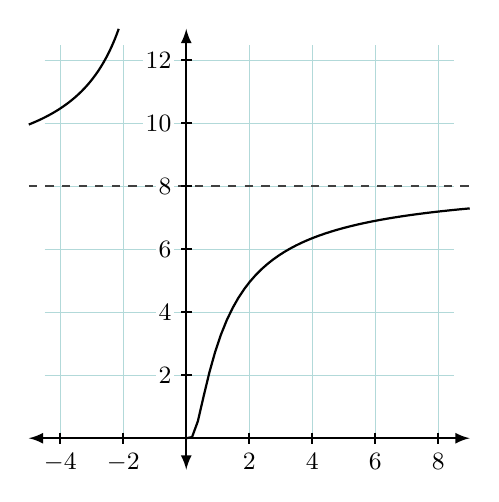
\begin{tikzpicture}[xscale=.4,yscale=.4,declare function={f(\x)=3*e^(1-(1/\x));} ,baseline=(current bounding box.north)]
            \draw[step=2,style=help lines,] (-4.5,0) grid (8.5,12.5);
            \draw[latex-latex, thick] (-5,0)--(9,0);
            \draw[latex-latex, thick] (0,-1)--(0,13);
            
            \draw[-,thick,dashed,color=gray!50!black] (-5,8) -- (9,8);
            
            \foreach \x in {-4,-2,2,4,6,8}
                \draw[thick] (\x,5pt) -- (\x,-5pt) node [below=.7mm,fill=white,inner sep=1pt] {\small$\x$};
            \foreach \y in {2,4,6,8,10,12}
                \draw[thick] (5pt,\y) -- (-5pt,\y) node [left=.7mm,fill=white,inner sep=1pt] {\small$\y$};
    
            
            \draw[thick] plot [samples=50,domain=.0001:9] ({\x},{f(\x)});
            \draw[thick] plot [samples=50,domain=-5:-2.1444] ({\x},{f(\x)});
            
            
        \end{tikzpicture}
    \end{flushright}
    
\end{questions}

\newpage

%add blurb about half carrying capicity is max growth rate for the DE.

\phantomsection\addcontentsline{toc}{subsection}{Logistic Differential Equations}
\subsection*{Logistic Differential Equations}

Before we talk about the LDE, first let's consider the following scenario:
\begin{questions}
    \question Let $N(t)$ be the population of wild coyotes in observed in a study of a wildlife reserve, with $t$ in years. The growth of the population is proportional to $650-N$. Initially, there are 300 coyotes. After two years, there is observed to be 500 coyotes. Find $N(3)$.
    
    \vspace{\stretch{1.2}}
\end{questions}

Correct answer! However, there is something \textit{inaccurate} about our work. What is it? Why?



\begin{center}
    \underline{A 'Normal' Differential Equation}
\end{center}
\begin{minipage}{0.45\linewidth}
    
        Differential Equation: $\displaystyle\frac{dy}{dt}=ky$
    
\end{minipage}
\hfill
\begin{minipage}{0.45\linewidth}
    
        General Solution: $\displaystyle y=Ce^{kt}$
    
\end{minipage}

This type of differential equation allows for \textbf{unlimited growth}. Obviously, we do not live in a world of infinites, so there cannot be an infinite number of coyotes as time goes on. We need a \textbf{carrying capacity}, $L$, to limit our growth. 


\begin{center}
    \underline{The Logistic Differential Equation}
\end{center}
\begin{minipage}{0.45\linewidth}
    
        Differential Equation:\\ 
        $\displaystyle\frac{dy}{dt}=ky\left(1-\frac{y}{L}\right)$ or $\displaystyle\frac{dy}{dt}=\frac{ky}{L}(L-y)$

\end{minipage}
\hfill
\begin{minipage}{0.45\linewidth}
    
        General Solution: $\displaystyle y=\frac{L}{Ce^{-kt}+1}$
    
\end{minipage}

\vspace{.25in}

%typo

\begin{center}
    \textbf{\large Memorize both forms of the differential equation and its general solution for the BC Exam!}
\end{center}


\newpage



\begin{questions}
    \setcounter{question}{1}
    \question 40 elk are released into a game refuge. After 5 years, the population of elk is observed to be 104. The game warden says that the refuge can support no more than 4000 elk at any given time.
    \begin{parts}
        \part Write a differential equation for the population of elk.
        \vspace{\stretch{1}}
        
        \part Write a model for the population, $P$, in terms of $t$. (Use the general solution, do not attempt to integrate!)
        \vspace{\stretch{1}}
    \end{parts}
    
    \question Find $\displaystyle\frac{d^2 y}{dx^2}$ for the general L.D.E. What can we deduce based on this function?
    \vspace{\stretch{1}}
\end{questions}


\textit{\footnotesize Solving for the general solution to a LDE requires an integration method not yet covered. We will circle back and derive it as an exercise later.}


\newpage
\phantomsection\addcontentsline{toc}{subsection}{Euler's Method}
\subsection*{Euler's Method}

% Make own section, Larger title, add 1-2 more examples/applications of EM. Prob own page.

\textbf{Euler's Method:} This is an method to approximate the particular solution of a differential equation $y'=F(x,\,y)$ that passes through $(x_0,\,y_0)$.

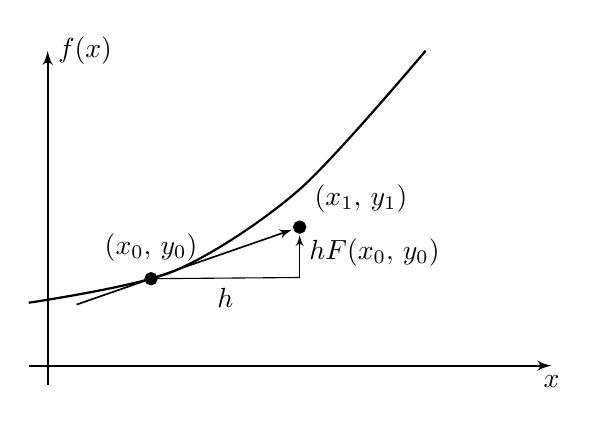
\begin{tikzpicture}[
    scale=.8,
    thick,
    >=latex',
    dot/.style = {
      draw,
      fill = black,
      circle,
      inner sep = 0pt,
      minimum size = 4pt
    }
  ]
  \coordinate (O) at (0,0);
  \draw[->] (-0.3,0) -- (8,0) coordinate[label = {below:$x$}] (xmax);
  \draw[->] (0,-0.3) -- (0,5) coordinate[label = {right:$f(x)$}] (ymax);
  \path[name path=x] (0.3,0.5) -- (6.7,4.7);
  \path[name path=y] plot[smooth] coordinates {(-0.3,1) (2,1.5) (4,2.8) (6,5)};
  \scope[name intersections = {of = x and y, name = i}]
    
    
    \draw plot[smooth] coordinates {(-0.3,1) (2,1.5) (4,2.8) (6,5)};
    \draw (i-1) node[dot, label = {above:$(x_0,\,y_0)$}] {};
    \draw (4,2.2) node[dot, label = {above right:$(x_1,\,y_1)$}] {};
    
    \draw[-,thin] (i-1) -- node[below] {$h$} (4,1.4);
    \draw[->,thin,shorten >=.1cm] (4,1.4) -- node[right] {$hF(x_0,\,y_0)$} (4,2.2);
    \draw[->,semithick,shorten <=-1cm,shorten >=.1cm] (i-1) -- (4,2.2);
    
  \endscope
\end{tikzpicture}

\begin{questions}
    \question Use Euler's Method to approximate the particular solution to the differential equation $y'=x-y$ passing through the point $(0,\,1)$. Use a step of $h=0.2.$
    
    \begin{parts}
        \part Perform three iterations.
        \vspace{\stretch{1}}
        
        \part approximate $y(0.8).$
        \vspace{\stretch{1}}
    \end{parts}
    
    \question Consider the differential equation $\displaystyle\frac{dy}{dx}=3x+2y+1$. Let $y=f(x)$ be a particular solution to the differential equation with initial condition $f(0)=2$. Use Euler's Method, starting at $x=0$, with step size of $\frac{1}{2}$, to approximate $f(1)$. (No Calc!)
    
    \vspace{\stretch{1.2}}
\end{questions}




\newpage
\phantomsection\addcontentsline{toc}{subsection}{Areas in the Plane}
\subsection*{Areas in the Plane}
\textbf{Warm up:} Determine the area between the curve and the $x$-axis for $y=x^2-x-6$ on $[-4,\,4].$
\vspace{\stretch{.75}}

\begin{tcolorbox}[title= AREA IN THE PLANE,colframe=black,sharp corners,colback=white,colbacktitle=white,coltitle=black,boxrule=1pt]

     If $f$ and $g$ are continuous with $f(x)\ge g(x)$ throughout $[a,\,b]$, then the area between the curves $y=f(x)$ and $y=g(x)$ from $a$ to $b$ is the integral
     \[A=\int_a^b\left[f(x)-g(x)\right]\,dx\].
    
\end{tcolorbox}

\textbf{Examples:}
\begin{questions}
    \question Determine the area of the region bounded by the graphs of $y=x^2+3,\,y=x+1,\,x=0,$ and $x=2$.
    \vspace{\stretch{1}}
    
    \question Determine the area of the region enclosed by the parabola $y=2-x^2$ and the line $y=x$.
    \vspace{\stretch{1}}
    
    \newpage
    
    \question The sine and cosine curves intersect infinitely many times, bounding regions of equal areas. Find the area of one of these regions.
    \vspace{\stretch{1}}
    
    \question Determine the area of the region enclosed by the graphs of $x=3-y^2$ and $x=y+1$.
    \vspace{\stretch{1}}
    
    \question Determine the area of the region $R$ in the first quadrant that is bounded above by $y=\sqrt{x}$ and below by the $x$-axis and the line $y=x-2$. Use geometry to simplify this computation.
    \vspace{\stretch{1}}
\end{questions}



\newpage
\phantomsection\addcontentsline{toc}{subsection}{Volumes of Revolution}
\subsection*{Volumes of Revolution}
\textbf{Problem 1:} Sketch the region bounded by the $x$-axis, the $y$-axis, the line $x=4$, and the line $y=3$. What is the volume of the solid formed when the region is revolved around the $x$-axis?
\vspace{\stretch{1}}

\textbf{Problem 2:} What is the volume of the solid formed by revolving around the $x$-axis the region bounded by the axes and the line $y=-x+4$?
\vspace{\stretch{1}}

\textbf{Problem 3:} Consider the shape of the region that is generated if $y=x^2$ on the interval $[0,\,3]$ is revolved around the $x$-axis. What is the volume of this solid?
\vspace{\stretch{.5}}

\newpage


\begin{tcolorbox}[title= VOLUME OF A SOLID OF REVOLUTION,colframe=black,sharp corners,colback=white,colbacktitle=white,coltitle=black,boxrule=1pt]

     The volume of a solid of known integrable cross section can be found by rotating the region bounded by $y=f(x),\,y=0,\,x=a,$ and $x=b$ about the $x$-axis using the integral
     \[V=\pi\int_a^b\left(f(x)\right)^2\,dx.\]
     This is commonly referred to as the \textbf{disc method}.
    
\end{tcolorbox}
\textbf{Examples:}
\begin{questions}
    \question Find the volume of the solid formed by revolving the region bounded by the graph of $f(x)=\sqrt{\sin x}$ and the $x$-axis $\left(0\le x\le\pi\right)$ about the $x$-axis.
    \vspace{\stretch{1}}
    
    \question Find the volume of the solid formed by revolving the region bounded by $f(x)=2-x^2$ and the $x$-axis about the $x$-axis.
    \vspace{\stretch{1}}
    
    \question Find the volume of the solid formed by revolving the region bounded by $y=x^{2/3},\, x=0$ and $y=1$ about the $y$-axis.
    \vspace{\stretch{1}}
    
    \newpage
    
    \question Find the volume of the solid formed by revolving the region bounded by $f(x)=2-x^2$ and $g(x)=1$ about the line $y=1$.
    \vspace{\stretch{1}}

\end{questions}

\begin{tcolorbox}[title= VOLUME OF A REGION USING WASHERS,colframe=black,sharp corners,colback=white,colbacktitle=white,coltitle=black,boxrule=1pt]

     \[\text{Volume of a region}=\pi\int_a^b\left(\left[R(x)\right]^2-\left[r(x)\right]^2\right)\,dx.\]
     Where $R(x)$ is the radius of the outer washer, $r(x)$ is the inner radius, and the integral represents the height of the \textit{cylinder}.
    
\end{tcolorbox}

\textbf{Examples:}
\begin{questions}
    \question Find the volume of the solid formed by revolving the region bounded by the graphs of $y=\sqrt{x}$ and $y=x^2$ about the $x$-axis.
    \vspace{\stretch{1}}
    
    \question Find the volume of the solid generated by revolving the region bounded by the curves $y=x^2$ and $y=2-x^2$ about the $x$-axis.
    \vspace{\stretch{1}}
    
    \newpage
    
    \question Find the volume of the solid generated by revolving the region bounded the graphs of $y=x^2+1,\,y=0,\,x=0,$ and $x=1$ about the $y$-axis.
    \vspace{\stretch{1}}
    
    \question The region in the first quadrant enclosed by the $y$-axis and the graphs of $y=\cos x$ and $y=\sin x$ is revolved around the $x$ axis to form a solid. Find its volume.
    \vspace{\stretch{1}}
    
    \question The area of the region bounded by the graphs of $y=\sqrt{x}$ and $y=x^2$ in the first quadrant is revolved around the line $x=3$. Find the volume of this solid.
    \vspace{\stretch{1}}
    
\end{questions}

\newpage

\begin{tcolorbox}[title= VOLUME OF KNOWN CROSS SECTION,colframe=black,sharp corners,colback=white,colbacktitle=white,coltitle=black,boxrule=1pt]

    The volume of a solid of known integrable cross section area $A(x)$ from $x=a$ to $x=b$ is the integral of $A$ from $a$ to $b$,
    \[V=\int_a^b A(x)\,dx.\]
    
\end{tcolorbox}
\textbf{Examples:}

\begin{questions}
    \question A pyramid 3m high has congruent triangular sides and a square base that is 3m on each side. Each cross section of the pyramid parallel to the base is a square. Find the volume of the pyramid.
    
    \vspace{\stretch{1}}
    
    \question A mathematician has a paperweight made so that its base is the shape of the region between the $x$-axis and one arch of the curve $y=2\sin x$. Each cross section cut perpendicular to the $x$-axis is a semi-circle whose diameter runs from the $x$-axis to the curve. Find the volume of the paperweight.
    \vspace{\stretch{1}}
\end{questions}



\newpage
\phantomsection\addcontentsline{toc}{subsection}{Arc Length}
\subsection*{Arc Length}
\begin{tcolorbox}[title= DEFINITION OF ARC LENGTH,colframe=black,sharp corners,colback=white,colbacktitle=white,coltitle=black,boxrule=1pt]

    Let the function $y=f(x)$ represent a smooth curve on the interval $[a,\,b]$. The \textbf{arc length} of $f$ between $a$ and $b$ is
    \[s=\int_a^b\sqrt{1+\left[f'(x)\right]^2}\,dx.\]
    Similarly, for a function $x=g(y)$, we get
    \[s=\int_a^b\sqrt{1+\left[g'(y)\right]^2}\,dy.\]
    
\end{tcolorbox}

\textbf{Note:} Very few integrals involving arc length can be computed by hand. For the homework, use a calculator after the initial setup.\\
\\
\textbf{Examples:} Find the length of the arc for the given function on the specified interval
\begin{questions}
    \question $\displaystyle x^2=(y-1)^{3}$ on $[0,\,8]$.
    \vspace{\stretch{1}}
    
    
    
    \question $\displaystyle y=\ln(\cos x)$ from $x=0$ to $x=\pi/4$. \textbf{(Do by hand)}
    \vspace{\stretch{1}}
    
    \question $\displaystyle y=\frac{x^3}{6}+\frac{1}{2x}$ on $\displaystyle\left[\frac{1}{2},\,2\right]$.
    \vspace{\stretch{1}}
\end{questions}

\newpage
\phantomsection\addcontentsline{toc}{section}{Advanced Integration Techniques}
\phantomsection\addcontentsline{toc}{subsection}{Integration Review}
\subsection*{Integration Review}
\begin{center}
    \textbf{Three Similar Integrals}
\end{center}
\begin{parts}
    \begin{minipage}{0.3\linewidth}
        \part $\displaystyle\int\frac{4}{x^2+9}\,dx$
    \end{minipage}
    \hfill
    \begin{minipage}{0.3\linewidth}
        \part $\displaystyle\int\frac{4x}{x^2+9}\,dx$
    \end{minipage}
    \hfill
    \begin{minipage}{0.3\linewidth}
        \part $\displaystyle\int\frac{4x^2}{x^2+9}\,dx$
    \end{minipage}


\vspace{\stretch{1}}

\newpage

\begin{center}
\textbf{Tricky Substitutions:}     
\end{center}


\begin{minipage}{.45\linewidth}
    \part $\displaystyle\int\frac{x^2}{\sqrt{16-x^6}}\,dx$    
\end{minipage}
\hfill
\begin{minipage}{.45\linewidth}
    \part $\displaystyle\int (\cot x)\left[\ln(\sin x)\right] \,dx$
\end{minipage}


\vspace{\stretch{1}}


\end{parts}



\newpage
\phantomsection\addcontentsline{toc}{subsection}{Integration by Parts}
\subsection*{Integration by Parts}
Up to this point, we have \textit{still} been doing only the simple-ish integrals. They can get more complicated, but with a bit of practice, not necessarily harder. Today, we are going to learn how to integrate the product of two different transcendental functions. A.k.a, \textbf{undo the product rule}!

\begin{tcolorbox}[title= INTEGRATION BY PARTS THEOREM,colframe=black,sharp corners,colback=white,colbacktitle=white,coltitle=black,boxrule=1pt]

    If $u$ and $v$ are functions of $x$ and have continuous derivatives, then
    \[\int u\,dv=uv-\int v\,du.\]
    
\end{tcolorbox}

\textbf{Hint:} Try letting $dv$ be the more complicated part of the integrand that fits a basic integration rule.

\textbf{Examples:} Evaluate the following integrals
\begin{questions}
    \question $\displaystyle\int xe^x\,dx$
    \vspace{\stretch{1}}
    
    \begin{minipage}{0.45\linewidth}
        \question $\displaystyle\int x^2\ln x\,dx$
    \end{minipage}
    \hfill
    \begin{minipage}{.45\linewidth}
        \question $\displaystyle\int_0^1 \arcsin x\,dx$
    \end{minipage}
    
    \vspace{\stretch{1}}
    
    \question $\displaystyle \int x^2\sin x\,dx$
    
    \vspace{\stretch{1}}
    
    
    \newpage
    
    
    \question Using the \textbf{Tabular Method}:
    \begin{parts}
        \begin{minipage}{.45\linewidth}
            \part $\displaystyle\int x^2\sin x\,dx$
        \end{minipage}
        \hfill
        \begin{minipage}{.45\linewidth}
            \part $\displaystyle\int x^2 e^{2x}\,dx$
        \end{minipage}
    \end{parts}
    
    \vspace{\stretch{1}}
    
    \question $\displaystyle\int e^{3x}\cos x\,dx$
    
    \vspace{\stretch{1}}
\end{questions}


%make one page (one day)


\newpage
\phantomsection\addcontentsline{toc}{subsection}{Trigonometric Combinations}
\subsection*{Trigonometric Combinations}
\textbf{Overarching Goal of this Section:} Rewrite an integrand with one factor of cosine and some expression involving sine (or vise versa).\\
\\
\textbf{Odd Power Examples:}
\begin{parts}
    \begin{minipage}{.45\linewidth}
            \part $\displaystyle\int \sin^5 x\,dx$
        \end{minipage}
        \hfill
        \begin{minipage}{.45\linewidth}
            \part $\displaystyle\int \sin^3 x\cos^2 x\,dx$
        \end{minipage}
\end{parts}

\vspace{\stretch{1}}

\textbf{Even Power Examples:}
\begin{parts}
    \begin{minipage}{.45\linewidth}
            \part $\displaystyle\int \sin^2 x\,dx$
        \end{minipage}
        \hfill
        \begin{minipage}{.45\linewidth}
            \part $\displaystyle\int \cos^4 x\,dx$
        \end{minipage}
\end{parts}

\vspace{\stretch{1}}

\newpage

\textbf{Integrals involving Secant and Tangent:}
\begin{parts}
    \begin{minipage}{.45\linewidth}
            \part $\displaystyle\int \tan^6 x\sec^4 x\,dx$
        \end{minipage}
        \hfill
        \begin{minipage}{.45\linewidth}
            \part $\displaystyle\int \tan^5 x\sec^7 x\,dx$
        \end{minipage}
\end{parts}
\vspace{\stretch{1}}

\textbf{Using Other Identities:} Evaluate $\displaystyle\int \cos^2 x\tan^3 x\,dx$
\vspace{\stretch{.6}}

\newpage
\phantomsection\addcontentsline{toc}{subsection}{Trigonometric Substitution}
\subsection*{Trigonometric Substitution}
Integrals containing a term of the form $\displaystyle\sqrt{a^2-x^2},\,\sqrt{a^2+x^2},\,$ or $\displaystyle\sqrt{x^2-a^2}$ you can often rewrite using a substitution involving a trigonometric function.\\
\\
For example, let's consider the form $\displaystyle\sqrt{a^2-x^2}$ for some $a>0$. Choose $x=a\sin\theta$ for your substitution.

\[\sqrt{a^2-x^2}=\hspace{3.5in}\]

We will produce the substituions for the rest as we go and complete the table at the end of the section.

\vspace{.5in}

\textbf{Examples:} Evaluate each of the following integrals using a trigonometric substitution.

\begin{questions}
    \question $\displaystyle\int\frac{1}{x^2\sqrt{4-x^2}}\,dx$
    \vspace{\stretch{1}}
    
    \question $\displaystyle\int_0^3 \frac{1}{\sqrt{9+x^2}}\,dx$
    \vspace{\stretch{1}}
    
    \newpage
    
    \question $\displaystyle\int\frac{\sqrt{x^2-25}}{x}\,dx$

    
\end{questions}

\vspace{5in}


\begin{longtable}[b]{|C{3.667cm}|C{3.667cm}|C{3.667cm}|C{3.7cm}|}
    \hline
    \textbf{Expression}\Tstrut\Bstrut & \textbf{Trig Substitution}\Tstrut\Bstrut & \textbf{Interval}\Tstrut\Bstrut & \textbf{Identity}\Tstrut\Bstrut \\\hline
    & & & \\
    $\displaystyle\sqrt{a^2-x^2}$\Tstrut\Bstrut & & & \\
    & & & \\\hline
    & & & \\
    $\displaystyle\sqrt{a^2+x^2}$\Tstrut\Bstrut & & & \\
    & & & \\\hline
    & & & \\
    $\displaystyle\sqrt{x^2-a^2}$\Tstrut\Bstrut & & & \\
    & & & \\\hline
    
\end{longtable}

\textbf{Closing Remark:} You do not always \textit{have} to use T.S., however, it does provide a procedure that will always work.


\newpage
\phantomsection\addcontentsline{toc}{subsection}{Partial Fraction Decomposition}
\subsection*{Partial Fraction Decomposition}



Let's start off this section with a simple observation:
    \[\displaystyle\frac{3}{x+2}-\frac{2}{x-5}\,\, = \,\, \hspace{.2in}\textit{\footnotesize     some math, idk}\hspace{.2in} \,\,=\,\, \frac{x-19}{x^2-3x-10}\]
Now, let's try to evaluate $\displaystyle\int\frac{x-19}{x^2-3x-10}\,dx$. Unfortunately, there is not going to be a way to integrate this rational function in it's current form. You can try, but the $u$-substitution does not differ by a constant. RIP, I know. \\
\\
But, $\displaystyle\int\frac{x-19}{x^2-3x-10}\,dx=\int\left(\frac{3}{x+2}-\frac{2}{x-5}\right)\,dx=3\ln|x+2|-2\ln|x-5|+C$. \textit{\footnotesize Wow!}

\vspace{.25in}

\textbf{Examples:} \textbf{(Warning!! These are long)}
\begin{questions}
    \question Use partial fraction decomposition to reduce to distinct linear factors.\\
    $\displaystyle\int\frac{1}{x^2+x-2}\,dx$
    \vspace{\stretch{1}}
    
    \newpage
    
    \question Closely examine this one before starting PFD.\\
    $\displaystyle\int\frac{2x^3-4x^2-15x+5}{x^2-2x-8}\,dx$
    \vspace{\stretch{1}}
    
    \newpage
    
    \question Evaluate.\\
    $\displaystyle\int\frac{5x^2+20x+6}{x^3+2x^2+x}\,dx$
    
    \newpage
    
    \question Hmm, there seems to be something different about this one...\\
    $\displaystyle\int\frac{2x^3-2x-8}{(x^2-x)(x^2+4)}\,dx$
    
    \vspace{\stretch{1}}
    
    \question Solve the differential equation: $\displaystyle\frac{dy}{dx}=ky\left(1-\frac{y}{L}\right)$
    
    \vspace{\stretch{.7}}
\end{questions}



\newpage
\phantomsection\addcontentsline{toc}{subsection}{Improper Integrals}
\subsection*{Improper Integrals}
\textbf{Recall} the following two conditions from theorems earlier this year:
\begin{enumerate}

    \item The definition of the definite integral requires that the interval $[a,\,b]$ is finite.
    \item The Fundamental Theorem of Calculus requires that the function is continuous on $[a,\,b]$.
\end{enumerate}
Integrals that do not possess these properties are called \textbf{improper integrals}, and we can still compute them with the addition of limits!

\begin{tcolorbox}[title= DEFINITION OF IMPROPER INTEGRALS WITH INFINITE BOUNDS,colframe=black,sharp corners,colback=white,colbacktitle=white,coltitle=black]

    \begin{enumerate}
        \item If $f$ is continuous on the interval $[a,\,\infty)$, then 
        \[\int_a^\infty f(x)\,dx=\lim_{b\to\infty}\int_a^b f(x)\,dx.\]
        \item If $f$ is continuous on the interval $(-\infty,\,b]$, then 
        \[\int_{-\infty}^b f(x)\,dx=\lim_{a\to-\infty}\int_a^b f(x)\,dx.\]
        \item If $f$ is continuous on the interval $(-\infty,\,\infty)$, then 
        \[\int_{-\infty}^\infty f(x)\,dx=\int_{-\infty}^c f(x)\,dx + \int_c^{\infty} f(x),\,dx\]
        where $c$ is any real number.
    \end{enumerate}
    
    If the limit exists, then it is said that improper integral \textbf{converges}, otherwise, it \textbf{diverges}. In the third case, if either of the integrals on the right diverge, then so does the one on the left.

\end{tcolorbox}

\textbf{Examples:}
\begin{questions}
    \question Evaluate $\displaystyle\int_1^\infty \frac{1}{x}\,dx$.
    \vspace{\stretch{1}}
    
    \newpage
    
    \begin{minipage}{.45\linewidth}
        \question $\displaystyle\int_1^\infty e^{-x}\,dx$
    \end{minipage}
    \hfill
    \begin{minipage}{.45\linewidth}
        \question $\displaystyle\int_1^\infty (1-x)e^{-x} \,dx$
    \end{minipage}

    \vspace{\stretch{1}}
    
    
    \question $\displaystyle\int_{-\infty}^\infty\frac{e^x}{1+e^{2x}}\,dx$

    \vspace{\stretch{1}}

\end{questions}

\newpage


\begin{tcolorbox}[title= DEFINITION OF IMPROPER INTEGRALS WITH INFINITE DISCONTINUITIES,colframe=black,sharp corners,colback=white,colbacktitle=white,coltitle=black]

    \begin{enumerate}
        \item If $f$ is continuous on the interval $[a,b)$ and has an infinite discontinuity at $b$, then 
        \[\int_a^b f(x)\,dx=\lim_{c\to b^-}\int_a^c f(x)\,dx.\]
        \item If $f$ is continuous on the interval $(a,b]$ and has an infinite discontinuity at $a$, then 
        \[\int_a^b f(x)\,dx=\lim_{c\to a^+}\int_c^b f(x)\,dx.\]
        \item If $f$ is continuous on the interval $[a,b]$ except for some $c$ in $(a,b)$ at which $f$ has an infinite discontinuity, then 
        \[\int_a^b f(x)\,dx=\int_{a}^c f(x)\,dx + \int_c^{b} f(x),\,dx.\]
    \end{enumerate}
    
    If the limit exists, then it is said that improper integral \textbf{converges}, otherwise, it \textbf{diverges}. In the third case, if either of the integrals on the right diverge, then so does the one on the left.

\end{tcolorbox}


\textbf{Examples:}
\begin{questions}
    \begin{minipage}{.45\linewidth}
        \question Evaluate $\displaystyle\int_0^1\frac{dx}{\sqrt[3]{x}}$.    
    \end{minipage}
    \hfill
    \begin{minipage}{.45\linewidth}
        \question Evaluate $\displaystyle\int_0^2\frac{dx}{x^3}$.
    \end{minipage}
    
    \vspace{\stretch{1}}
    
    \newpage
    
    \question Evaluate $\displaystyle\int_{-1}^2\frac{dx}{x^3}$.
    
    \vspace{\stretch{1}}
    
    
    
    \question Evaluate $\displaystyle\int_0^\infty\frac{dx}{\sqrt{x}(x+1)}.$
    
    \vspace{\stretch{1}}
\end{questions}


\begin{tcolorbox}[title= A SPECIAL IMPROPER INTEGRAL,colframe=black,sharp corners,colback=white,colbacktitle=white,coltitle=black]

    \[\int_1^\infty\frac{dx}{x^p}=
    \begin{cases}
        \frac{1}{p-1} & \text{if }p>1\\
        \text{diverges} & \text{if }p\le1
    \end{cases}\]

\end{tcolorbox}


\newpage
\phantomsection\addcontentsline{toc}{section}{Sequences \& Series}
\phantomsection\addcontentsline{toc}{subsection}{Sequences Basics}
\subsection*{Sequences Basics}
Mathematically, a \textbf{sequence} is defined as a function whose domain is the set of positive integers (or, as some might claim, the \textbf{natural numbers} $\mathbb{N}$). Although a sequence is a function, it is common to represent sequences by subscript notation.\\ \\
Example:
$\begin{matrix}
     1, & 2, & 3, & 4, & 5, & ... , & n, & ... & \hspace{.5in}\text{Each }a_{n}\text{ is a }\textbf{term}\text{ of the sequence}.\\
     \Big\downarrow & \Big\downarrow & \Big\downarrow & \Big\downarrow & \Big\downarrow & \Big\downarrow & \Big\downarrow & \Big\downarrow &   \\
     a_{1}, & a_{2}, & a_{3}, & a_{4}, & a_{5}, & ...\, , & a_{n}, & ...\, , & \hspace{.5in}\text{The number }a_{n}\text{ is called the }\textbf{nth term}.
\end{matrix}$\\
\\
\\

%\vspace{.35in}

\textbf{\textit{Finding Patterns}} Describe a pattern for each of the following sequences. Then use your description to write a formula for the $n$th term of each sequence. As $n$ increases, do the terms appear to be approaching a limit?\\ 

\begin{parts}
    \begin{minipage}{0.45\linewidth}
        \part $1,\, \frac{1}{2},\, \frac{1}{4},\, \frac{1}{8},\, \frac{1}{16},\, ...$
    \end{minipage}
    \hfill
    \begin{minipage}{0.45\linewidth}
        \part $1,\, \frac{1}{2},\, \frac{1}{6},\, \frac{1}{24},\, \frac{1}{120},\, ...$
    \end{minipage}
    
    \vspace{\stretch{.7}}
    
    \begin{minipage}{0.45\linewidth}
        \part $10,\, \frac{10}{3},\, \frac{10}{6},\, \frac{10}{10},\, \frac{10}{15},\, ...$
    \end{minipage}
    \hfill
    \begin{minipage}{0.45\linewidth}
        \part $\frac{1}{4},\, \frac{4}{9},\, \frac{9}{16},\, \frac{16}{25},\, \frac{25}{36},\, ...$
    \end{minipage}
    
    \vspace{\stretch{.7}}
    
    \begin{minipage}{0.45\linewidth}
        \part $\frac{3}{7},\, \frac{5}{10},\, \frac{7}{13},\, \frac{9}{16},\, \frac{11}{19},\, ...$
    \end{minipage}
    \hfill
    \begin{minipage}{0.45\linewidth}
        \part Let $\displaystyle a_{n}=\left\{\frac{4n}{3-2n}\right\}$. List out the first five terms, then estimate $\displaystyle\lim_{n\to\infty}a_{n}$.
    \end{minipage}
    
    \vspace{\stretch{1}}
    
\end{parts}


\newpage


\begin{tcolorbox}[title= DEFINITION OF THE LIMIT OF A SEQUENCE,colframe=black,sharp corners,colback=white,colbacktitle=white,coltitle=black]

    Let $L$ be a real number. The \textbf{limit} of a sequence $\{a_n\}$ is $L$, written as, 
    \[\lim_{n\to\infty}a_n=L\]
    if for each $\epsilon>0$, there exists $M>0$ such that $|a_n-L|<\epsilon$ whenever $n>M$. If the limit $L$ of a sequence exists, then the sequence \textbf{converges} to $L$. If the limit of a sequence does not exist, then the sequence \textbf{diverges}.

\end{tcolorbox}
\vspace{.1in}
\noindent I know what you are thinking:  \textit{translation please!1??!?}\\
\\
\underline{Convergent}: When a sequence has a limit that approaches some real number $L$.

\noindent\underline{Divergent}: A sequence that does \textit{not} have a limit.\\
\\
\noindent Possibilities:
\begin{questions}
    \question If $\displaystyle\lim_{n\to\infty}a_n=\infty$, then $\{a_n\}$ diverges to infinity.
    \question If $\displaystyle\lim_{n\to\infty}a_n=-\infty$, then $\{a_n\}$ diverges to negative infinity.
    \question If $\displaystyle\lim_{n\to\infty}a_n=L$, a real finite number, then $\{a_n\}$ converges to $L$.
    \question If $\displaystyle\lim_{n\to\infty}a_n$ oscillates between two fixed numbers, then $\{a_n\}$ diverges by oscillation.
\end{questions}

\vspace{1cm}

\noindent\textbf{Example}: Does the sequence $\displaystyle a_{n}=\left\{\frac{\ln\sqrt{n}}{n}\right\}$ converge or diverge? If convergent, where to?

\newpage

As we just saw, L'Hopital's Rule becomes a very important part of determining convergence of \textit{interesting} sequences.


\begin{tcolorbox}[colframe=black,sharp corners,colback=white,boxrule=.25mm]
    Some Important Limits to Know:
    \begin{itemize}
    
        \item[] $\displaystyle\lim_{n\to\infty}\frac{c}{n}=$ \vspace{.15in}
        \item[] $\displaystyle\lim_{n\to\infty}\frac{\ln{n}}{n}=$\vspace{.15in}
        \item[] $\displaystyle\lim_{n\to\infty}\sqrt[n]{n}=$\vspace{.15in}
        \item[] $\displaystyle\lim_{n\to\infty}x^{n}=$\vspace{.15in}
        \item[] $\displaystyle\lim_{n\to\infty}x^{\frac{1}{n}}=$\vspace{.15in}
        \item[] $\displaystyle\lim_{n\to\infty}\left(1+\frac{x}{n}\right)^{n}=$\vspace{.15in}
        \item[] $\displaystyle\lim_{n\to\infty}\frac{x^{n}}{n!}=$\vspace{.15in}
        \item[] $\displaystyle\lim_{n\to\infty}\frac{n!}{x^n}=$\vspace{.15in}
        
    
    
    \end{itemize}
    

\end{tcolorbox}
\vspace{.1in}
\noindent\textbf{Examples:}\\
Determine whether the following sequences converge or diverge.
\begin{parts}

    \begin{minipage}{0.3\linewidth}
        \part $\displaystyle\frac{1}{2},\,\frac{2}{3},\,\frac{3}{4},\,\frac{4}{5},\,...$
    \end{minipage}
    \hfill
    \begin{minipage}{0.3\linewidth}
        \part $\displaystyle\frac{1}{2},\,\frac{1}{4},\,\frac{1}{8},\,\frac{1}{16},\,...$
    \end{minipage}
    \hfill
    \begin{minipage}{0.3\linewidth}
        \part $\displaystyle a_{n}=3+(-1)^n$
    \end{minipage}
    
    \vspace{\stretch{1}}
        
    \begin{minipage}{0.3\linewidth}
        \part $\displaystyle a_{n}=\frac{n}{1-2n}$
    \end{minipage}
    \hfill
    \begin{minipage}{0.3\linewidth}
        \part $\displaystyle a_{n}=\frac{\ln n}{n}$
    \end{minipage}
    \hfill
    \begin{minipage}{0.3\linewidth}
        \part $\displaystyle a_{n}=\frac{n!}{(n+2)!}$
    \end{minipage}
    
    \vspace{\stretch{1}}


\end{parts}

\newpage
\phantomsection\addcontentsline{toc}{subsection}{Series \& Convergence}
\subsection*{Series \& Convergence}


\begin{tcolorbox}[title= DEFINITION OF CONVERGENT AND DIVERGENT SERIES,colframe=black,sharp corners,colback=white,colbacktitle=white,coltitle=black]

    For the infinite series $\displaystyle\sum_{n=1}^{\infty}a_n$, the \textbf{\textit{n}th partial sum} is given by
    \[S_n=a_1+a_2+a_3+...+a_n.\]
    If the sequence of partial sums $\{S_n\}$ converges to $S$, then the series $\displaystyle\sum_{n=1}^{\infty}a_n$ \textbf{converges}. The limit $S$ is called the \textbf{sum of the series}. 
    \[S_n=a_1+a_2+a_3+...+a_n \text{   where   }S=\sum_{n=1}^{\infty}a_n\]
    If $\{S_n\}$ diverges, then the series \textbf{diverges}.

\end{tcolorbox}
\vspace{.1in}

\noindent\textbf{Example: Convergent and Divergent Series}\\
Find the sequence of partial sums $S_1,\, S_2,\, S_3$ and an expression for $S_n$ for each of the following series. Determine its convergence or divergence.
\begin{parts}
    \part $\displaystyle\sum_{n=1}^{\infty}\frac{1}{2^n}=\frac{1}{2}+\frac{1}{4}+\frac{1}{8}+\frac{1}{16}+...$
    \vspace{\stretch{1}}
    
    \part $\displaystyle\sum_{n=1}^{\infty}\left(\frac{1}{n}-\frac{1}{n+1}\right)=\left(1-\frac{1}{2}\right)+\left(\frac{1}{2}-\frac{1}{3}\right)+\left(\frac{1}{3}-\frac{1}{4}\right)+...$
    \vspace{\stretch{1}}
    
    \part $\displaystyle\sum_{n=1}^{\infty}1=1+1+1+1+...$
    \vspace{\stretch{.2}}
\end{parts}


\noindent A \textbf{telescoping series} has the form $(b_1-b_2)+(b_2-b_3)+(b_3-b_4)+...$ therefore $S_n=b_1-b_{n+1}$. A telescoping series converges if and only if $b_n\rightarrow$ a finite number as $n\rightarrow\infty$. In which case, $\displaystyle S=b_1-\lim_{n\to\infty}b_{n+1}$.

\newpage


\noindent\textbf{Example: A Telescoping Series In Disguise}\\
Find the sum of the series $\displaystyle\sum_{n=1}^{\infty}\frac{2}{4n^2-1}$.
\vspace{\stretch{1}}


\phantomsection\addcontentsline{toc}{subsection}{Geometric Series}
\subsection*{Geometric Series}
Specific Example: $3+3\cdot2+3\cdot2^2+3\cdot2^3+...$\\
General Form: $\displaystyle\sum_{n=0}^{\infty}ar^n=a+ar+ar^2+...+ar^n+...$

\begin{tcolorbox}[title= CONVERGENCE OF A GEOMETRIC SERIES,colframe=black,sharp corners,colback=white,colbacktitle=white,coltitle=black]

    \begin{enumerate}
        \item A geometric series with ratio $r$ diverges if $|r|\ge1$.
        \item If $0<|r|<1$, then the series converges to the sum
        \[\displaystyle\sum_{n=0}^{\infty}ar^n=\frac{a}{1-r},\, 0<|r|<1.\]
    \end{enumerate}

\end{tcolorbox}
\vspace{.1in}

\noindent\textbf{Example: Convergent and Divergent Geometric Series}\\
Determine the convergence or divergence of the series. If it converges, find its sum.
\begin{parts}
    \begin{minipage}{0.45\linewidth}
        \part $\displaystyle\sum_{n=0}^{\infty}\frac{3}{2^n}$
    \end{minipage}
    \hfill
    \begin{minipage}{0.45\linewidth}
        \part $\displaystyle\sum_{n=0}^{\infty}\left(\frac{3}{2}\right)^n$
    \end{minipage}
    \vspace{\stretch{1}}
\end{parts}

\begin{tcolorbox}[title= PROPERTIES OF INFINITE SERIES,colframe=black,sharp corners,colback=white,colbacktitle=white,coltitle=black]

    Let $\displaystyle\sum a_n$ and $\displaystyle\sum b_n$ be convergent series, and let $A$, $B$, and $c$ be real numbers. If $\displaystyle\sum a_n=A$ and $\displaystyle\sum b_n=B$, the the following series converge to the indicated sums
    \[1.\, \, \sum_{n=1}^{\infty}ca_n=cA \hspace{2in}2.\, \, \sum_{n=1}^{\infty}\left(a_n\pm b_n\right)=A\pm B\]

\end{tcolorbox}

\newpage
\phantomsection\addcontentsline{toc}{subsection}{\textit{n}th-Term Test for Divergence}
\subsection*{\textit{n}th-Term Test for Divergence}
\begin{tcolorbox}[title= LIMIT OF THE nTH TERM OF A SERIES,colframe=black,sharp corners,colback=white,colbacktitle=white,coltitle=black]

    \begin{center}
    Let $\displaystyle\sum a_n$ converge, then $\displaystyle\lim_{n\to\infty}a_n=0$.
    
    
    If $\displaystyle\lim_{n\to\infty}a_n\ne0$, then $\displaystyle\sum a_n$  diverges.
    \end{center}
    
\end{tcolorbox}
We commonly abbreviate the name of this theorem to the "Divergence Test".\\
\\
\noindent\textbf{Example: Using the Divergence Test}\\
Determine the convergence or divergence of each series.
\begin{parts}
    \begin{minipage}{0.23\linewidth}
        \part $\displaystyle\sum_{n=0}^{\infty}2^n$
    \end{minipage}
    \hfill
    \begin{minipage}{0.23\linewidth}
        \part $\displaystyle\sum_{n=1}^{\infty}\frac{n!}{2n!+1}$
    \end{minipage}
    \hfill
    \begin{minipage}{0.23\linewidth}
        \part $\displaystyle\sum_{n=1}^{\infty}\frac{1}{n}$
    \end{minipage}
    \vspace{\stretch{1}}
\end{parts}

\noindent\textbf{Example: Bouncing Ball Problem}\\
A ball is dropped from a height of 6 feet and begins bouncing as shown in the figure below. The height of each bounce is three-fourths the height of the previous bounce. Find the total vertical distance traveled by the ball.


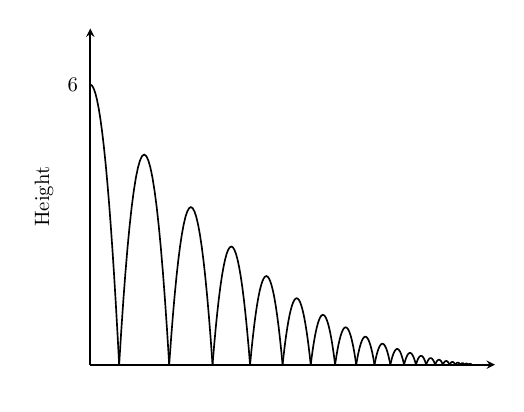
\begin{tikzpicture}[scale=.75,
  declare function={
    bounce(\hz,\idx) = \hz*(3/4)^\idx;
    duration(\hz,\idx) = sqrt(2*\hz/9.81)*(1+sqrt(3)*(1-sqrt(3/4)^\idx)/(1-sqrt(3/4)));
    offset(\hz,\idx) = duration(\hz,\idx-1)+(duration(\hz,\idx)-duration(\hz,\idx-1))/2;
    flight(\hz,\idx,\t) = bounce(\hz,\idx)-9.81/2*(\t-offset(\hz,\idx))^2;
  }
]
  \begin{axis}[
      xmin=0, xmax=20,
      ymin=0, ymax=12,
      thick,
      axis lines=left,
      xtick={14.047},
      ytick={10},
      %xtick={{duration(10,8)}},
      xticklabels={},
      yticklabels={6},
      xlabel={},
      ylabel={Height},
      tick style=transparent,
  ]
    \addplot[domain=0:{duration(20,0)}] {bounce(10,0)-9.81/2*\x^2};
    \foreach \p in {1,...,20} {
      \addplot[domain={duration(10,\p-1)}:{duration(10,\p)}] {flight(10,\p,\x)}; 
    }
    
  \end{axis}
\end{tikzpicture}

\vspace{\stretch{1}}




\newpage
\phantomsection\addcontentsline{toc}{subsection}{Integral Test \& \textit{p}-Series}
\subsection*{Integral Test \& \textit{p}-Series}
Let's start this section with an example...\\
\\
Consider the series: $\displaystyle\sum_{n=1}^\infty \frac{1}{n^2}=\frac{1}{1^1}+\frac{1}{2^2}+\frac{1}{3^2}+...$\\
\\
First, verify that the Divergence Test is inconclusive and that this is not a geometric series.\\
\vspace{\stretch{1}}


Does the series converge?
\vspace{\stretch{3}}


\newpage

\begin{tcolorbox}[title= THE INTEGRAL TEST,colframe=black,sharp corners,colback=white,colbacktitle=white,coltitle=black]

    If $a_n=f(n)$ and $f$ is continuous, positive, and decreasing on $[1,\infty)$, then
    \[\sum_{n=1}^{\infty}a_n\hspace{.35in}\text{and}\hspace{.35in} \int_1^{\infty}f(x)\,dx\]
    either both converge or diverge.

\end{tcolorbox}
\vspace{.1in}

\noindent\textbf{THREE IMPORTANT FACTS}:
\begin{questions}
    \question They do \textbf{not} converge to the same value! In the example we just did:
    \[\displaystyle\sum_{n=1}^\infty \frac{1}{n^2}=\frac{\pi^2}{6}\ne1=\int_1^\infty\frac{1}{x^2}\,dx\]
    
    \question We can start at other indices (limits of integration).
    
    \question $f$ does not have to be always decreasing, only \textbf{ultimately} decreasing.
\end{questions}
\vspace{.1in}

\noindent\textbf{Examples:} Determine the convergence or divergence of each series.
\begin{parts}
    \part $\displaystyle\sum_{n=1}^{\infty}\frac{n}{n^2+1}$
    \vspace{\stretch{1}}
    
    \part $\displaystyle\sum_{n=1}^{\infty}\frac{5}{2n^2+2}$
    \vspace{\stretch{1}}
    
    \part $\displaystyle\sum_{n=2}^{\infty}\frac{1}{n\ln(n)}$
    \vspace{\stretch{1}}
\end{parts}

\newpage

\begin{tcolorbox}[title= DEFINITION OF A $p$-SERIES,colframe=black,sharp corners,colback=white,colbacktitle=white,coltitle=black]

    A series of the form \[\displaystyle\sum_{n=1}^\infty \frac{1}{n^p}=\frac{1}{1^p}+\frac{1}{2^p}+\frac{1}{3^p}+...\] is a \textbf{\textit{p}-series}, where $p$ is a positive constant. For $p=1$, the series \[\sum_{n=1}^\infty\frac{1}{n}=\frac{1}{1}+\frac{1}{2}+\frac{1}{3}+...\]
    is called the \textbf{harmonic series}. A \textbf{general harmonic series} is of the form $\displaystyle\sum_{n=1}^\infty\frac{1}{an+b}$.

\end{tcolorbox}
\begin{tcolorbox}[title= CONVERGENCE OF A $p$-SERIES,colframe=black,sharp corners,colback=white,colbacktitle=white,coltitle=black]

    A series of the form \[\displaystyle\sum_{n=1}^\infty \frac{1}{n^p}=\frac{1}{1^p}+\frac{1}{2^p}+\frac{1}{3^p}+...\] converges if $p>1$ and diverges if $0<p\le1$.

\end{tcolorbox}
\vspace{.1cm}

\noindent\textbf{Examples:}
\begin{questions}
    \question Determine the convergence or divergence of each series.
    \begin{parts}
        \begin{minipage}{0.23\linewidth}
            \part $\displaystyle\sum_{n=1}^{\infty}\frac{1}{\sqrt{n}}$
        \end{minipage}
        \hfill
        \begin{minipage}{0.23\linewidth}
            \part $\displaystyle\sum_{n=1}^{\infty}\frac{1}{n\sqrt{n}}$
        \end{minipage}
        \hfill
        \begin{minipage}{0.23\linewidth}
            \part $\displaystyle\sum_{n=1}^{\infty}\frac{1}{n^{1.04}}$
        \end{minipage}
        \vspace{\stretch{1}}
    \end{parts}

    \question Find the positive values of $p$ for which the series converges:

    \begin{parts}
        \begin{minipage}{0.45\linewidth}
            \part $\displaystyle\sum_{n=2}^{\infty}\frac{1}{n\left(\ln(n)\right)^p}$
        \end{minipage}
        \hfill
        \begin{minipage}{0.45\linewidth}
            \part $\displaystyle\sum_{n=1}^{\infty}\frac{n}{(1+n^2)^p}$
        \end{minipage}
        \vspace{\stretch{3}}
    \end{parts}

\end{questions}




\newpage
\phantomsection\addcontentsline{toc}{subsection}{Comparison of Series}
\subsection*{Comparison of Series}


One motif of the series (which you probably didn't notice) that we have been looking at is that they are relatively simple. However, with any slight complications, we can no longer apply the tests in our arsenal. For example:

\begin{enumerate}
    \item $\displaystyle\sum_{n=0}^\infty\frac{1}{2^n}$ is geometric, but $\displaystyle\sum_{n=0}^{\infty}\frac{n}{2^n}$ is not.
    \item $\displaystyle\sum_{n=1}^{\infty}\frac{1}{n^3}$ is a $p$-series, but $\displaystyle\sum_{n=1}^\infty\frac{1}{n^3+1}$ is not.
    \item $\displaystyle a_n=\frac{n}{(n^2+3)^2}$ is easily integrated, but $\displaystyle b_n=\frac{n^2}{(n^2+3)^2}$ is not.
\end{enumerate}

\vspace{.07in}

\begin{tcolorbox}[title= THE DIRECT COMPARISON TEST,colframe=black,sharp corners,colback=white,colbacktitle=white,coltitle=black]

    Let $0<a_n\le b_n$ for all $n$.\\
    \begin{enumerate}
        \item If $\displaystyle\sum_{n=1}^\infty b_n$ converges, then $\displaystyle\sum_{n=1}^\infty a_n$ converges.
        \item If $\displaystyle\sum_{n=1}^\infty a_n$ diverges, then $\displaystyle\sum_{n=1}^\infty b_n$ diverges.
    \end{enumerate}

\end{tcolorbox}
\vspace{.07in}
\noindent\textbf{THREE IMPORTANT FACTS}:
\begin{questions}
    \question Your comparison does not always have to be greater than or equal to $a_n$, just as long as it is \textbf{ultimately} greater than (or less than) the original.
    \question To prove a series is convergent, your comparison must be \textbf{larger}.
    \question To prove a series is divergent, your comparison must be \textbf{smaller}.
\end{questions}

\noindent\textbf{Examples:} Determine the convergence or divergence of each series.
\begin{parts}
    \begin{minipage}{0.45\linewidth}
        \part $\displaystyle\sum_{n=1}^\infty \frac{1}{2+3^n}$
    \end{minipage}
    \hfill
    \begin{minipage}{0.45\linewidth}
        \part $\displaystyle\sum_{n=1}^\infty \frac{1}{2+\sqrt{n}}$
    \end{minipage}
\end{parts}

\newpage

\begin{tcolorbox}[title= THE LIMIT COMPARISON TEST,colframe=black,sharp corners,colback=white,colbacktitle=white,coltitle=black]

    Suppose that $a_n>0,\,b_n>0$, and
    \[\lim_{n\to\infty}\left(\frac{a_n}{b_n}\right)=L\]
    where $L$ is \textit{finite} and \textit{positive}. Then the two series $\displaystyle\sum a_n$ and $\displaystyle\sum b_n$ either both converge or both diverge.

\end{tcolorbox}
\vspace{.1in}
\noindent\textbf{Examples: Using the Limit Comparison Test}\\
Determine the convergence or divergence of $\displaystyle\sum_{n=1}^{\infty}\frac{\sqrt{n}}{n^2+1}$.
\vspace{\stretch{1}}


Determine the convergence or divergence of $\displaystyle\sum_{n=1}^\infty\frac{n2^n}{4n^3+1}$.
\vspace{\stretch{1}}




\newpage
\phantomsection\addcontentsline{toc}{subsection}{Alternating Series}
\subsection*{Alternating Series}
The simplest of alternating series can be a geometric series. The following example is easy to determine its convergence since we know that the geometric series test can be applied:
\[\sum_{n=0}^{\infty}\left(-\frac{1}{2}\right)^n=1-\frac{1}{2}+\frac{1}{4}-\frac{1}{8}+\frac{1}{16}-\cdots\]

\vspace{.07in}

\begin{tcolorbox}[title= THE ALTERNATING SERIES TEST,colframe=black,sharp corners,colback=white,colbacktitle=white,coltitle=black]

    Let $a_n>0$. The alternating series
    \[\sum_{n=1}^\infty(-1)^n\, a_n\hspace{.15in}\text{and}\hspace{.15in}\sum_{n=1}^\infty(-1)^{n+1}\,a_n\]
    converge if the following conditions are met.\\
    \begin{enumerate}
        \item $\displaystyle\lim_{n\to\infty}a_n=0$
        \item $\displaystyle a_{n+1}\le a_n$, for all $n$
    \end{enumerate}

\end{tcolorbox}
\vspace{.1in}
\noindent\textbf{ONE IMPORTANT FACT}:
\begin{questions}
    \question The second condition in the Alternating series test can be modified to require only that $0<a_{n+1}\le a_n$ for all $n$ greater than some integer $N$.
\end{questions}
\vspace{.1in}

\noindent\textbf{Examples:}\\
Determine the convergence or divergence of each series.
\begin{parts}
    \begin{minipage}{0.45\linewidth}
        \part $\displaystyle\sum_{n=1}^\infty (-1)^{n+1}\frac{1}{2+3^n}$
    \end{minipage}
    \hfill
    \begin{minipage}{0.45\linewidth}
        \part $\displaystyle\sum_{n=1}^\infty \frac{n}{(-2)^{n-1}}$
    \end{minipage}
\end{parts}

\newpage



\noindent\textbf{Example: When the AST Fails}
\begin{questions}
    \question $\displaystyle\sum_{n=1}^\infty \frac{(-1)^{n+1}(n+1)}{n}=\frac{2}{1}-\frac{3}{2}+\frac{4}{3}-\frac{5}{4}+\frac{6}{5}-\cdots$
    \vspace{\stretch{1}}
    
    \question $\displaystyle\frac{2}{1}-\frac{1}{1}+\frac{2}{2}-\frac{1}{2}+\frac{2}{3}-\frac{1}{3}+\frac{2}{4}-\frac{1}{4}+\cdots$
    \vspace{\stretch{1}}
\end{questions}



\noindent\textbf{\Large Alternating Series Remainder:}
\begin{tcolorbox}[title= THE ALTERNATING SERIES REMAINDER THEOREM,colframe=black,sharp corners,colback=white,colbacktitle=white,coltitle=black]

    If a convergent alternating series satisfies the condition $\displaystyle a_{n+1}\le a_n$, then the absolute value of the reminder $R_N$ involved in approximating the sum $S$ by $S_N$ is less than (or equal to) the first neglected term. That is,
    \[\left|S-S_N\right|=\left|R_N\right|\le a_{N+1}\]

\end{tcolorbox}
\vspace{.1in}
The reason why this is the case is hard to conceptualize, so perhaps a proof might help.\\
\\
\noindent \textbf{Proof:} The series obtained by deleting the first $N$ terms of the given series satisfies the conditions of the conditions of the Alternating series test and has a sum of $R_N$.
\begin{align*}
    R_N = S-S_N &= \displaystyle\sum_{n=1}^{\infty}(-1)^{n+1}a_n-\sum_{n=1}^{N}(-1)^{n+1}a_n\\
     &= \displaystyle(-1)^{N}a_{N+1} + (-1)^{N+1}a_{N+2} + (-1)^{N+2}a_{N+3} + \cdots\\
     &= \displaystyle(-1)^{N}\left(a_{N+1}-a_{N+2}+a_{N+3}-\cdots\right)\\
    |R_N| &= a_{N+1}-a_{N+2}+a_{N+3}-a_{N+4}+a_{N+5}-\cdots\\
    &= a_{N+1}-\left(a_{N+2}-a_{N+3}\right)-\left(a_{N+4}-a_{N+5}\right)-\cdots\le a_{N+1}
\end{align*}
Consequently, $\displaystyle\left|S-S_N\right|=|R_N|\le a_{N+1}$, which establishes the theorem.



\newpage

\noindent\textbf{Examples:}\\
\begin{questions}
    \question Consider the following series:
    \[\displaystyle\sum_{n=1}^{\infty}(-1)^{n+1}\left(\frac{1}{n!}\right)=\frac{1}{1!}-\frac{1}{2!}+\frac{1}{3!}-\frac{1}{4!}+\frac{1}{5!}-\frac{1}{6!}+\cdots\]
    \begin{parts}
        \part Approximate the sum of the series using the first six terms.
        
        
        
        \part What is the error associated with this approximation?
        
        
        
        \part What is the interval for which the true sum of the series, $S$, must lie within? (Use the previous two answers)
        
        \vspace{\stretch{1}}
    \end{parts}
    
    \question Consider the series $\displaystyle\sum_{n=0}^\infty \frac{(-1)^n \cdot 3^{n+1}}{2^{2n}}$.
    \begin{parts}
        \part Find the maximum error associated with the approximation of $S_4$.
        \part How many terms would it take for the error to be less than $\frac{1}{200}$?
    \end{parts}
    
    
    \vspace{\stretch{1}}
    
    
    
    
\end{questions}





\newpage


\phantomsection\addcontentsline{toc}{subsection}{Conditional and Absolute Convergence}
\subsection*{Absolute and Conditional Convergence}
Occasionally, we run into series that have both positive and negative terms but is \textbf{not} an alternating series. For example:



\[\displaystyle\sum_{n=1}^{\infty}\frac{\sin n}{n^2}=\frac{\sin1}{1}+\frac{\sin2}{4}+\frac{\sin3}{9}+\cdots\]
In order to obtain any information about the convergence of this series, let's instead consider
\[\displaystyle\sum_{n=1}^{\infty}\left|\frac{\sin n}{n^2}\right|.\]
\vspace{\stretch{1}}

\begin{tcolorbox}[title= ABSOLUTE CONVERGENCE,colframe=black,sharp corners,colback=white,colbacktitle=white,coltitle=black]

    If the series $\displaystyle\sum\left|a_n\right|$ converges, then the series $\displaystyle\sum a_n$ also converges.

\end{tcolorbox}
\vspace{.1in}
Note that the opposite is \textbf{not} true. For instance, the \textbf{alternating harmonic series} converges by the alternating series test. Yet the harmonic series diverges. This is called \textbf{conditional convergence.}
\[\sum_{n=1}^\infty \frac{(-1)^{n+1}}{n}=\frac{1}{1}-\frac{1}{2}+\frac{1}{3}-\frac{1}{4}+\cdots\]


\newpage

\begin{tcolorbox}[title= DEFINITIONS OF ABSOLUTE AND CONDITIONAL CONVERGENCE,colframe=black,sharp corners,colback=white,colbacktitle=white,coltitle=black]

    \begin{enumerate}
        \item $\displaystyle\sum a_n$ is \textbf{absolutely convergent} if $\displaystyle\sum\left|a_n\right|$ converges.
        \item $\displaystyle\sum a_n$ is \textbf{conditionally convergent} if $\displaystyle\sum a_n$ converges but $\displaystyle\sum\left|a_n\right|$ diverges.
    \end{enumerate}

\end{tcolorbox}
\vspace{.1in}
\noindent\textbf{Practice:}\\
Determine whether each of the series is convergent or divergent. Classify any convergent series as absolutely or conditionally convergent.
\begin{questions}
    
    \begin{minipage}{0.45\linewidth}
    \question $\displaystyle\sum_{n=0}^\infty \frac{(-1)^n n!}{2^n}$
    \end{minipage}
    \hfill
    \begin{minipage}{0.45\linewidth}
    \question $\displaystyle\sum_{n=1}^\infty \frac{(-1)^n}{\sqrt{n}}$
    \end{minipage}
    \vspace{\stretch{1}}
    
    \begin{minipage}{0.45\linewidth}
    \question $\displaystyle\sum_{n=1}^\infty \frac{(-1)^{n(n+1)/2} n!}{3^n}$
    \end{minipage}
    \hfill
    \begin{minipage}{0.45\linewidth}
    \question $\displaystyle\sum_{n=1}^\infty \frac{(-1)^n}{\ln(n+1)}$
    \end{minipage}
    \vspace{\stretch{1}}
    
    
\end{questions}


\newpage
\phantomsection\addcontentsline{toc}{subsection}{Ratio and Root Tests}
\subsection*{Ratio and Root Tests}

\begin{tcolorbox}[title= THE RATIO TEST,sharp corners,colback=white,colbacktitle=white,coltitle=black]

    Let     $\displaystyle\sum a_n$ be a series with nonzero terms.
    \begin{enumerate}
        \item $\displaystyle\sum a_n$ converges absolutely if $\displaystyle\lim_{n\to\infty}\left|\frac{a_{n+1}}{a_n}\right|<1$.
        \item $\displaystyle\sum a_n$ diverges if $\displaystyle\lim_{n\to\infty}\left|\frac{a_{n+1}}{a_n}\right|>1$ or $\displaystyle\lim_{n\to\infty}\left|\frac{a_{n+1}}{a_n}\right|=\infty$.
        \item The Ratio Test is inconclusive if $\displaystyle\lim_{n\to\infty}\left|\frac{a_{n+1}}{a_n}\right|=1$.
    \end{enumerate}

\end{tcolorbox}
\vspace{.1in}
\noindent\textbf{ONE IMPORTANT FACT}:
\begin{questions}
    \question This is not the one stop shop for tests of convergence, but \textit{usually} is for series involving factorials or exponentials.
\end{questions}
\vspace{.1in}

\noindent\textbf{Example:}\\
Determine the convergence or divergence of each series.
\begin{parts}
    \begin{minipage}{0.45\linewidth}
        \part $\displaystyle\sum_{n=0}^\infty \frac{2^n}{n!}$
    \end{minipage}
    \hfill
    \begin{minipage}{0.45\linewidth}
        \part $\displaystyle\sum_{n=1}^\infty \frac{n^n}{n!}$
    \end{minipage}
    
    \vspace{\stretch{1}}
    
    \part $\displaystyle\sum_{n=1}^\infty (-1)^n \frac{\sqrt{n}}{n+1}$
    
    \vspace{\stretch{1}}
    
\end{parts}

\newpage

\begin{tcolorbox}[title= THE ROOT TEST,colframe=black,sharp corners,colback=white,colbacktitle=white,coltitle=black]

    Let
    $\displaystyle\sum a_n$ be a series.
    \begin{enumerate}
        \item $\displaystyle\sum a_n$ converges absolutely if $\displaystyle\lim_{n\to\infty}\sqrt[n]{\left|a_n\right|}<1$.
        \item $\displaystyle\sum a_n$ diverges if $\displaystyle\lim_{n\to\infty}\sqrt[n]{\left|a_n\right|}>1$ or $\displaystyle\lim_{n\to\infty}\sqrt[n]{\left|a_n\right|}=\infty$.
        \item The Root Test is inconclusive if $\displaystyle\lim_{n\to\infty}\sqrt[n]{\left|a_n\right|}=1$.
    \end{enumerate}

\end{tcolorbox}
\vspace{.1in}

\noindent\textbf{ONE IMPORTANT FACT}:
\begin{questions}
    \question The Root Test is always inconclusive for a $p$-series. So don't even bother.
\end{questions}
\vspace{.1in}
\noindent\textbf{Example:}\\
Test the series for convergence or divergence. Afterwards, \textit{try} the Ratio Test to see why it is not ideal.
$\displaystyle\sum_{n=1}^\infty \frac{e^{2n}}{n^n}$


\newpage

\noindent\textbf{\Large Strategies for Testing Series}\\
\\
You have learned 10 strategies for testing a series for convergence or divergence. 

\textbf{Guidelines for Testing a Series:}
\begin{enumerate}
    \item Does the $n$th term approach 0? If not, the series diverges.
    \item Is the series one of the special types (geo, $p$-series, telescoping, alternating)?
    \item Can the integral test, ratio test, or root test be applied?
    \item Can the series be compared favorably to one of the special types?
\end{enumerate}

\noindent\textbf{Example: Applying Strategies}
\begin{parts}
    \begin{minipage}{0.45\linewidth}
        \part $\displaystyle\sum_{n=1}^{\infty}\frac{n+1}{3n+1}$
    \end{minipage}
    \hfill
    \begin{minipage}{0.45\linewidth}
        \part $\displaystyle\sum_{n=1}^{\infty}\left(\frac{\pi}{6}\right)^n$
    \end{minipage}
    
    \vspace{\stretch{1}}
    
    \begin{minipage}{0.45\linewidth}
        \part $\displaystyle\sum_{n=1}^{\infty}ne^{-n^2}$
    \end{minipage}
    \hfill
    \begin{minipage}{0.45\linewidth}
        \part $\displaystyle\sum_{n=1}^{\infty}\frac{1}{3n+1}$
    \end{minipage}
    
    \vspace{\stretch{1}}
    
    \newpage
    
    \begin{minipage}{0.45\linewidth}
        \part $\displaystyle\sum_{n=1}^{\infty}(-1)^n\frac{3}{4n+1}$
    \end{minipage}
    \hfill
    \begin{minipage}{0.45\linewidth}
        \part $\displaystyle\sum_{n=1}^{\infty}\frac{n!}{10^n}$
    \end{minipage}
    \vspace{\stretch{1}}
    \part $\displaystyle\sum_{n=1}^{\infty}\left(\frac{n+1}{2n+1}\right)^n$
    \vspace{\stretch{1}}


\end{parts}


\newpage
\phantomsection\addcontentsline{toc}{subsection}{Taylor Polynomials \& Approximations}
\subsection*{Taylor Polynomials \& Approximations}
The goal is to show polynomial functions can be used to approximate any elementary function. To do this, we require the following two conditions to be true about our function $f$ and the polynomial approximation $P$:
\[f(c)=P(c)\hspace{2in}f'(c)=P'(c).\]

\begin{center}
    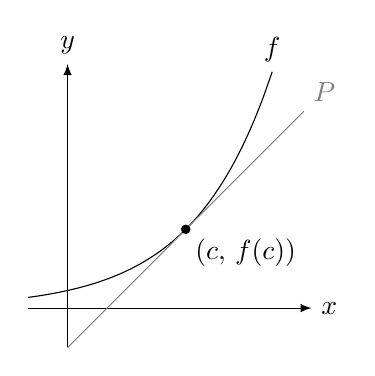
\begin{tikzpicture}
        \draw[-latex] (-.5,0)--(3.1,0) node[right]{$x$};
        \draw[-latex] (0,-.5)--(0,3.1) node[above] {$y$};
        \draw[] plot[smooth, domain=-.5:ln(3)+1.5] (\x, {e^(\x-1.5)}) node[anchor=south] {$f$};
        \draw[color=gray] plot[domain=0:3] (\x,{\x-.5}) node[anchor=south west] {$P$};
        \filldraw (1.5,1) circle (1.5pt) node[anchor=north west] {$(c,\,f(c))$};
        
    \end{tikzpicture}
\end{center}


The approximating polynomial is said to be \textbf{expanded about \textit{c}} or \textbf{centered at \textit{c}}. It should make sense that we require the slopes to match as there are an infinite number of polynomials that pass through $(c,\,f(c))$. This constraint, at the very least, makes the approximation look somewhat similar to $f$ at that point.\\
\\

\noindent\textbf{Introductory Example: First-Degree Polynomial Approximation of $\mathbf{f(x)=e^{x}}$: }\\
For the function $f(x)=e^x$, find a first degree polynomial function $P_1(x)=a_0+a_1 x$ whose value and slope agree with the value of the slope of $f$ at $x=0$.

\vspace{\stretch{1}}


    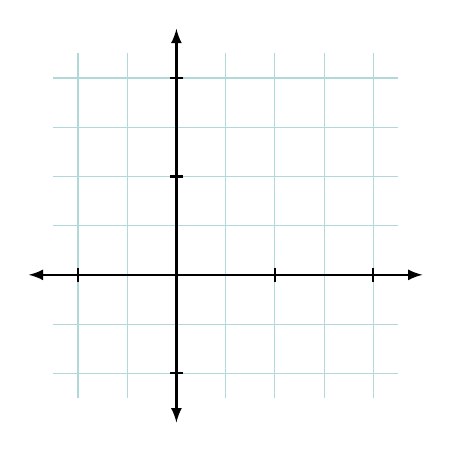
\begin{tikzpicture}[scale=1.25]
        \draw[style=help lines, step=.5] (-1.25,-1.25) grid (2.25,2.25);
        \draw[latex-latex,thick](-1.5,0)--(2.5,0);
        \draw[latex-latex,thick](0,-1.5)--(0,2.5);
        \foreach \x in {-1,1,2}
            \draw[thick] (\x,2pt)--(\x,-2pt);
        \foreach \y in {-1,1,2}
            \draw[thick] (2pt,\y)--(-2pt,\y);    
    \end{tikzpicture}


\newpage

Based on $P_1$ found in example 1, we can see that our approximation fits relatively well for values of $x$ that are close to $c=0$. However, the further we move away from $(0,1)$, it is clear that our approximation will not be accurate whatsoever. How might we improve the accuracy even further?\\

Let's consider the following:

\begin{minipage}{0.45\linewidth}
    \[P_2(x)=1+x+\frac{1}{2}x^2\]
\end{minipage}
\hfill
\begin{minipage}{0.45\linewidth}
    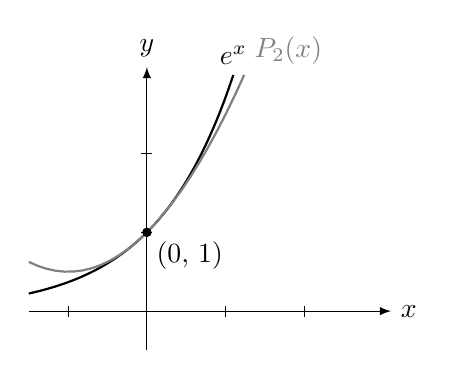
\begin{tikzpicture}
        \draw[-latex] (-1.5,0)--(3.1,0) node[right]{$x$};
        \draw[-latex] (0,-.5)--(0,3.1) node[above] {$y$};
        \foreach \x in {-1,1,2}
            \draw (\x,2pt)--(\x,-2pt);
        \foreach \y in {1,2}
            \draw (2pt,\y)--(-2pt,\y); 
        
        \draw[thick] plot[smooth, domain=-1.5:ln(3)] (\x, {e^(\x)}) node[anchor=south] {$e^x$};
        \draw[thick,color=gray] plot[domain=-1.5:1.236] (\x,{1+\x+.5*(\x)^2}) node[anchor=south west] {$P_2(x)$};
        \filldraw (0,1) circle (1.5pt) node[anchor=north west] {$(0,\,1)$};
        
    \end{tikzpicture}
\end{minipage}

\begin{minipage}{0.45\linewidth}
    \[P_3(x)=1+x+\frac{1}{2}x^2+\frac{1}{6}x^3\]
\end{minipage}
\hfill
\begin{minipage}{0.45\linewidth}
    \begin{tikzpicture}
        \draw[-latex] (-1.5,0)--(3.1,0) node[right]{$x$};
        \draw[-latex] (0,-.5)--(0,3.1) node[above] {$y$};
        \foreach \x in {-1,1,2}
            \draw (\x,2pt)--(\x,-2pt);
        \foreach \y in {1,2}
            \draw (2pt,\y)--(-2pt,\y); 
        
        \draw[thick] plot[smooth, domain=-1.5:ln(3)] (\x, {e^(\x)}) node[anchor=south east] {$e^x$};
        \draw[thick,color=gray] plot[domain=-1.5:1.125] (\x,{1+\x+.5*(\x)^2+1/6*(\x)^3}) node[anchor=south west] {$P_3(x)$};
        \filldraw (0,1) circle (1.5pt) node[anchor=north west] {$(0,\,1)$};
        
    \end{tikzpicture}
\end{minipage}

Clearly, $P_2$ is a better approximation than $P_1$, and $P_3$ more still. If we continue on, matching each $n$th derivative of $f(x)=e^x$ at $x=0$, we obtain the following:

\[P_n(x)=1+x+\frac{1}{2}x^2+\frac{1}{3!}x^3+\cdots+\frac{1}{n!}x^n\approx e^x\]

\vspace{.1in}

\begin{tcolorbox}[title= DEFINITIONS OF THE \textit{\textbf{n}}TH TAYLOR POLYNOMIAL AND \textbf{\textit{n}}TH MACLAURIN POLYNOMIAL,colframe=black,sharp corners,colback=white,colbacktitle=white,coltitle=black]

    If $f$ has $n$ derivatives at $c$, then the polynomial
    \[P_n(x)=f(c)+f'(c)(x-c)+\frac{f''(c)}{2!}(x-c)^2+\cdots+\frac{f^{(n)}(c)}{n!}(x-c)^n\]
    is called the \textbf{\textit{n}th Taylor Polynomial for \textit{f} at \textit{c}}. If $c=0$, then
    \[P_n(x)=f(0)+f'(0)(x)+\frac{f''(0)}{2!}x^2+\cdots+\frac{f^{(n)}(0)}{n!}x^n\]
    is also called the \textbf{\textit{n}th Maclaurin Polynomial for \textit{f}}. 

\end{tcolorbox}

\newpage

\noindent\textbf{Examples:}
\begin{questions}
    \question Find the $n$th Maclaurin polynomial for $f(x)=e^x$.
    \vspace{\stretch{1}}
    
    \question Find the Taylor polynomials $P_0,\,P_1,\,P_2,\,P_3,\,$and $P_4$ for $f(x)=\ln x$ centered at $c=1$.
    \vspace{\stretch{2.5}}
\end{questions}

\begin{minipage}{0.18\linewidth}
    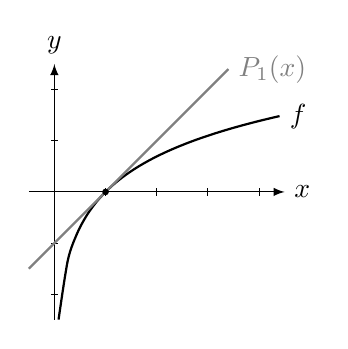
\begin{tikzpicture}[scale=.65]
        \draw[-latex] (-.5,0)--(4.5,0) node[right]{$x$};
        \draw[-latex] (0,-2.5)--(0,2.5) node[above] {$y$};
        \foreach \x in {1,2,3,4}
            \draw (\x,2pt)--(\x,-2pt);
        \foreach \y in {-2,-1,1,2}
            \draw (2pt,\y)--(-2pt,\y); 
        
        \draw[thick] plot[smooth, domain=e^(-2.5):4.4] (\x, {ln(\x)}) node[anchor=west] {$f$};
        \draw[thick,color=gray] plot[domain=-.5:3.4] (\x,{\x-1}) node[right] {$P_1(x)$};
        \filldraw (1,0) circle (1.5pt);
        
    \end{tikzpicture}
    \end{minipage}
    \hfill
    \begin{minipage}{0.18\linewidth}
        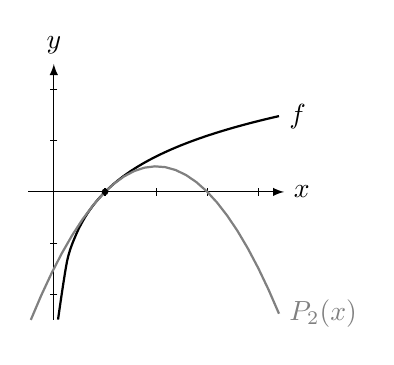
\begin{tikzpicture}[scale=.65]
            \draw[-latex] (-.5,0)--(4.5,0) node[right]{$x$};
            \draw[-latex] (0,-2.5)--(0,2.5) node[above] {$y$};
            \foreach \x in {1,2,3,4}
                \draw (\x,2pt)--(\x,-2pt);
            \foreach \y in {-2,-1,1,2}
                \draw (2pt,\y)--(-2pt,\y); 
            
            \draw[thick] plot[smooth, domain=e^(-2.5):4.4] (\x, {ln(\x)}) node[anchor=west] {$f$};
            \draw[thick,color=gray] plot[domain=-.45:4.4] (\x,{(\x-1)-1/2*(\x-1)^2}) node[right] {$P_2(x)$};
            \filldraw (1,0) circle (1.5pt);
            
        \end{tikzpicture}
    \end{minipage}
    \hfill
    \begin{minipage}{0.18\linewidth}
        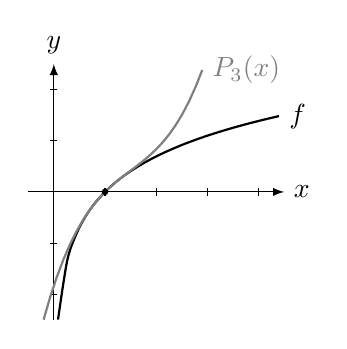
\begin{tikzpicture}[scale=.65]
            \draw[-latex] (-.5,0)--(4.5,0) node[right]{$x$};
            \draw[-latex] (0,-2.5)--(0,2.5) node[above] {$y$};
            \foreach \x in {1,2,3,4}
                \draw (\x,2pt)--(\x,-2pt);
            \foreach \y in {-2,-1,1,2}
                \draw (2pt,\y)--(-2pt,\y); 
            
            \draw[thick] plot[smooth, domain=e^(-2.5):4.4] (\x, {ln(\x)}) node[anchor=west] {$f$};
            \draw[thick,color=gray] plot[domain=-.2:2.9] (\x,{(\x-1)-1/2*(\x-1)^2+1/3*(\x-1)^3}) node[right] {$P_3(x)$};
            \filldraw (1,0) circle (1.5pt);
            
        \end{tikzpicture}
    \end{minipage}
    \hfill
    \begin{minipage}{0.18\linewidth}
        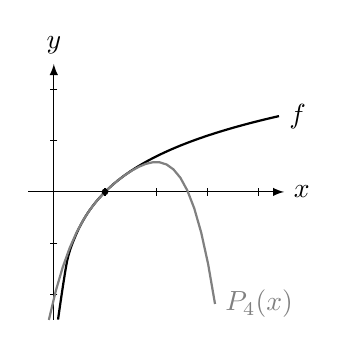
\begin{tikzpicture}[scale=.65]
            \draw[-latex] (-.5,0)--(4.5,0) node[right]{$x$};
            \draw[-latex] (0,-2.5)--(0,2.5) node[above] {$y$};
            \foreach \x in {1,2,3,4}
                \draw (\x,2pt)--(\x,-2pt);
            \foreach \y in {-2,-1,1,2}
                \draw (2pt,\y)--(-2pt,\y); 
            
            \draw[thick] plot[smooth, domain=e^(-2.5):4.4] (\x, {ln(\x)}) node[anchor=west] {$f$};
            \draw[thick,color=gray] plot[domain=-.097:3.15] (\x,{(\x-1)-1/2*(\x-1)^2+1/3*(\x-1)^3-1/4*(\x-1)^4}) node[right] {$P_4(x)$};
            \filldraw (1,0) circle (1.5pt);
            
        \end{tikzpicture}
    \end{minipage}
    
    \newpage


\begin{questions}
    \setcounter{question}{2}
    \question Find the Maclaurin Polynomials $P_n$ for $n=0,\,2,\,4,\,6$ for $f(x)=\cos x$. Then, use $P_6(x)$ to approximate the value of $\cos(0.1)$.
    \vspace{\stretch{1}}


    \question Find the third Taylor Polynomial for $f(x)=\sin x$, expanded about $c=\pi/6$.
    \vspace{\stretch{1}}

\end{questions}


\newpage
\phantomsection\addcontentsline{toc}{subsection}{Remainder of a Taylor Polynomial}
\subsection*{Remainder of a Taylor Polynomial}
As these are approximations, they will not be exactly equal to the original function. As we did with Alternating Series earlier this unit, we will revisit the concept of the \textbf{remainder}.

\begin{equation*}
    \tikzmark{exact}{f(x)} = \tikzmark{approx}{P_n(x)} + \tikzmark{remainder}{R_n(x)}
\end{equation*}
\begin{center}
    \begin{tikzpicture}[overlay, remember picture,node distance =.5cm]
        \node[,text width=3cm] (exactdescr) [below left=of exact ]{Exact value};
        \draw[,-latex] (exactdescr) to (exact);
        
        \node[,text width=3cm] (approxdescr) [below =of approx ]{Approx. value};
        \draw[,-latex] (approxdescr) to (approx);
        
        \node[,text width=2cm] (remainderdescr) [below right=of remainder ]{Remainder};
        \draw[,-latex] (remainderdescr) to (remainder);
        
    \end{tikzpicture}
\end{center}

\vspace{.2in}

So, $\displaystyle R_n(x)=f(x)-P_n(x)$. The absolute value of $\displaystyle R_n(x)$ is called the \textbf{error} associated with the approximation. That is,
\[\text{ERROR}=|R_n(x)|=|f(x)-P_n(x)|.\]

The following theorem is called \textbf{Taylor's Theorem}, and the remainder given in the theorem is called the \textbf{Lagrange form of the remainder}. You should know both names as synonymous.

\begin{tcolorbox}[title= TAYLOR'S THEOREM,colframe=black,sharp corners,colback=white,colbacktitle=white,coltitle=black]

    If a function $f$ is differentiable through order $n+1$ in an interval $I$ containing $c$, then, for each $x$ in $I$, there exists $z$ between $x$ and $c$ such that
    \[f(x)=f(c)+f'(c)(x-c)+\frac{f''(c)}{2!}(x-c)^2+\cdots+\frac{f^{(n)}(c)}{n!}(x-c)^n+R_n(x)\]
    where
    \[R_n(x)=\frac{f^{(n+1)}(z)}{(n+1)!}(x-c)^{n+1}.\]
    
\end{tcolorbox}
\vspace{.1in}
One thing to note when using this theorem is that $\displaystyle \left|R_n(x)\right|\le\frac{|x-c|^{n+1}}{(n+1)!}\max\left|f^{(n+1)}(z)\right|$ where $\max\left|f^{(n+1)}(z)\right|$ is the maximum value of $\left|f^{(n+1)}(z)\right|$ between $x$ and $c$.\\
\\
\noindent\textbf{Example:}\\
The third Maclaurin polynomial for $\sin x$ is given by $\displaystyle P_3(x)=x-\frac{x^3}{3!}$. Use Taylor's Theorem to approximate $\sin(0.1)$ by $P_3(0.1)$ and determine the error of the approximation.


\newpage

\noindent\textbf{More Examples:}
\begin{questions}
    \question The degree 4 Taylor Polynomial for $f(x)$ centered about $x=2$ is given by:
    \[P_4=9+\frac{1}{7}(x-2)^3+7(x-2)^4 .\]
    Using infromation from the graph of $y=f^{(5)}(x)$ below and the Lagrange error bound, approximate the maximum value of $\left|P_4(1.5)-f(1.5)\right|$.

    \vspace{\stretch{1}}

    \question asdflhdajlfhdfa;ldfhl;ajdfhjlahfjkldhajlfhjalhfdjl

    \vspace{\stretch{1}}

    \question Determine the degree of the Talyor Polynomial $P_n(x)$ expanded about $c=1$ that should be used to approximate $\ln(1.2)$ so that the error is less than 0.001.
    \vspace{\stretch{1}}
    
    \question Find an upper bound for the error of the $5^{\text{th}}$ degree polynomial approximation of $e$.
    \vspace{\stretch{1}}
    
    \question Let $\displaystyle f(x) = \sum_{n=1}^{\infty}\frac{x^n n^n}{n!}$ for all $x$ for which the series converges.
    \begin{parts}
        \begin{minipage}{0.45\linewidth}
            \part Use the first three terms of the series to approximate $\displaystyle f\left(\frac{-1}{3}\right)$.
        \end{minipage}
        \hfill
        \begin{minipage}{0.45\linewidth}
            \part Estimate the error involved in the approximation of part (a).
        \end{minipage}
    \end{parts}

    \vspace{\stretch{1}}
    
    \newpage
    
    %%% check this section!
    
    \begin{minipage}[t]{0.45\linewidth}
    \question Let $\displaystyle P_4(x)=1+\frac{x^2}{2}+\frac{x^4}{4!}$ be the fourth-degree Taylor Polynomial for $f$ about $x=0$. Using the information from the graph of $\displaystyle \left|f^{(5)}(x)\right|$ shown to the right, show that \[\displaystyle\left|P_4\left(\frac{1}{4}\right)-f\left(\frac{1}{4}\right)\right|<\frac{1}{3000}.\]
    \end{minipage}
    \hfill
    \begin{minipage}[t]{0.45\linewidth}
    \begin{center}
    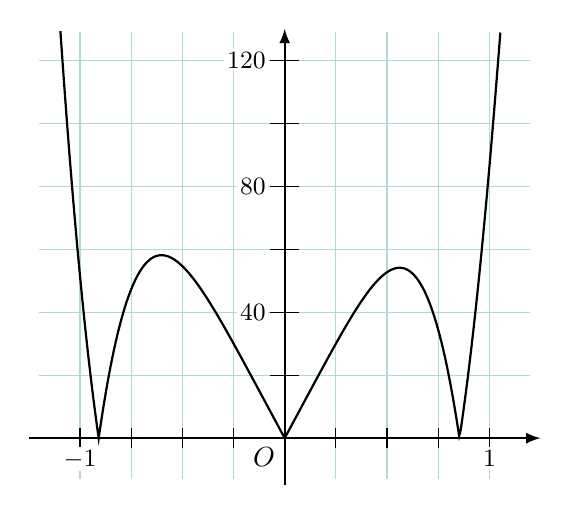
\begin{tikzpicture}[xscale=2.6,yscale=.04,declare function={f(\x)=abs(160*(\x^3)*sin((\x)^2 r)+2*\x*(16*(\x^4)-12)*cos((\x)^2 r)-96*\x*cos((\x)^2 r)-sin(\x r));},baseline=(current bounding box.north)]
        \draw[ystep=20,xstep=.25,style=help lines,] (-1.2,-13) grid (1.2,129);
        \draw[-latex, thick] (-1.25,0)--(1.25,0);
        \draw[-latex, thick] (0,-15)--(0,130);
        \foreach \x in {-1, -3/4, -.5, -.25, .25, .5, .75, 1}
            \draw (\x,90pt)--(\x,-90pt);
        \foreach \y in {20,40,60,80,100,120}
            \draw (2pt,\y)--(-2pt,\y);
        \foreach \x in {-1,1}
            \draw (\x,-1) node [below=.7mm,fill=white,inner sep=1pt] {\small$\x$};
        \foreach \y in {40,80,120}
            \draw (-.05,\y) node [left=.7mm,fill=white,inner sep=1pt] {\small$\y$};
        
        
        \draw[thick] plot [samples=300,domain=-1.0955:1.055] ({\x},{f(\x)});
        
        \node at (0,0) [below left] {$O$};
        
        
        
       %\draw[domain=-1.2:1.5, smooth,thick] plot (\x, {abs(160*(\x^3)*sin((\x)^2)+2*\x*(16*(\x^4)-12)*cos((\x)^2)-96*\x*cos((\x)^2)-sin(\x))});
    \end{tikzpicture}
    \end{center}
    \end{minipage}

    \vspace{\stretch{1}}
    
    \question The Taylor Series about $x=3$ for a certain function $f$ converges to $f(x)$ for all $x$ in the interval of convergence. The $n$th derivative of $f$ at $x=3$ is given by 
    \[\displaystyle f^{(n)}(3)\le\frac{(-1)^n \, n!}{5^n\, (n+3)}\text{for all \textit{n} and }f(3)=\frac{1}{3}.\]
    Show that $P_3(x)$ approximates $f(4)$ with an error less than $\displaystyle\frac{1}{4000}$.
    
    \vspace{\stretch{1}}


\end{questions}


\newpage
\phantomsection\addcontentsline{toc}{subsection}{Power Series}
\subsection*{Power Series}
In the previous section, we have been approximating some of our elementary functions using Taylor and Maclaurin Polynomials. We examined polynomials of first, second, third (and so on) degree and saw how closely they matched the original curve. The goal is going to be to move away from \textit{approximations} and instead represent a function \textit{exactly}.\\
\\
For example the function $f(x)=e^x$ can be represented exactly by an infinite series called a \textbf{power series}. The representation is
\[e^x=1+x+\frac{x^2}{2!}+\frac{x^3}{3!}+\cdots+\frac{x^n}{n!}+\cdots.\]
For each real number $x$, it can be shown that the infinite series on the right converges to the number $e^x$.\\


\begin{tcolorbox}[title= DEFINITIONS OF POWER SERIES,colframe=black,sharp corners,colback=white,colbacktitle=white,coltitle=black]

    If $x$ is a variable, then an infinite series of the form
    \[\sum_{n=0}^{\infty}a_n x^n=a_0 + a_1 x+a_2 x^2+a_3 x^3+\cdots+a_n x^n+\cdots\]
    is called a \textbf{power series}. More generally, an infinite series of the form
    \[\sum_{n=0}^{\infty}a_n (x-c)^n=a_0 + a_1 (x-c)+a_2 (x-c)^2+a_3 (x-c)^3+\cdots+a_n (x-c)^n+\cdots\]
    is called a \textbf{power series centered at \textit{c}}, where $c$ is a constant.

\end{tcolorbox}
\vspace{.1in}

\phantomsection\addcontentsline{toc}{subsection}{Radius and Interval of Convergence}
\subsection*{Radius and Interval of Convergence}
A power series in $x$ can be thought of as a function of $x$
\[f(x)=\sum_{n=0}^{\infty}a_n (x-c)^n\]
where the \textbf{domain of \textit{f}} is the set of all $x$ values for which the power series converges. The main goal of this section will be to determine where and when that happens.


\begin{tcolorbox}[title= CONVERGENCE OF A POWER SERIES,colframe=black,sharp corners,colback=white,colbacktitle=white,coltitle=black]

    For a power series centered at $c$, precisely one of the following is true.
    
    \begin{enumerate}
        \item The series converges only at $c$.
        \item There exists a real number $R>0$ such that the series converges absolutely for $|x-c|<R$, and diverges for $|x-c|>R$.
        \item The series converges absolutely for all $x$.
    \end{enumerate}
    The number $R$ is called the \textbf{radius of convergence} of the power series. If the series converges only at $c$, the radius of convergence is $R=0$, and if the series converges for all $x$, then the radius is $R=\infty$. The set of all values of $x$ for which the series converges is called the \textbf{interval of convergence} of the power series.

\end{tcolorbox}
\vspace{.1in}


\noindent\textbf{Examples:} Find the Radius of Convergence.
\begin{questions}
    \question $\displaystyle\sum_{n=0}^{\infty}n!x^n$
    \vspace{\stretch{1}}
    \question $\displaystyle\sum_{n=0}^{\infty}3(x-2)^n$
    \vspace{\stretch{1}}
    \question$\displaystyle\sum_{n=0}^{\infty}\frac{(-1)^n x^{2n+1}}{(2n+1)!}$
    \vspace{\stretch{1}}
    

\end{questions}

\newpage


\noindent\textbf{Endpoint of Convergence}: When $R$ is a finite value (such as in example 2 from the previous page), our theorem about convergence of power series never specifies what happens at the endpoints. As a result, they must be tested separately.\\
\\
\noindent\textbf{Examples:} Find the interval of Convergence.
\begin{questions}
    \question $\displaystyle\sum_{n=1}^{\infty}\frac{x^n}{n}$
    \vspace{\stretch{1}}
    
    \question$\displaystyle\sum_{n=1}^{\infty}\frac{x^n}{n^2}$
    \vspace{\stretch{1}}
\end{questions}

\newpage


\phantomsection\addcontentsline{toc}{subsection}{Differentiating and Integrating Power Series}
\subsection*{Differentiating and Integrating Power Series}
\begin{tcolorbox}[title= PROPERTIES OF FUNCTIONS DEFINED BY POWER SERIES,colframe=black,sharp corners,colback=white,colbacktitle=white,coltitle=black]

    If the function given by
    \begin{align*}
        f(x) &= \sum_{n=0}^{\infty}a_n (x-c)^n\\
        &= a_0 + a_1 (x-c)+a_2 (x-c)^2+a_3 (x-c)^3+\cdots+a_n (x-c)^n+\cdots
    \end{align*}
    has radius of convergence $R>0$, then, on the interval $(c-R,\,c+R)$, $f$ is differentiable (and therefore continuous). Moreover, the derivative and antiderivative of $f$ are as follows.
    
    
        \begin{align*}
            1.\hspace{.15in} f'(x) &= \sum_{n=0}^{\infty}na_n (x-c)^{n-1}\\
        &= a_1 + 2a_2 (x-c)+3a_3 (x-c)^2+4a_4 (x-c)^3+\cdots
        \end{align*}
        \begin{align*}
            2.\hspace{.15in}\int f(x)\,dx &= C+\sum_{n=0}^{\infty} a_n\frac{(x-c)^{n+1}}{n+1}\\
            &= C + a_0 (x-c)+ a_1\frac{(a-c)^2}{2}+a_2\frac{(x-c)^3}{3}+\cdots
        \end{align*}
    
    The \textit{radius of convergence} of the series obtained by differentiating or integrating a power series is the same as the original series. The \textit{interval of convergence}, however, may differ because of the behavior of the end points.
    
\end{tcolorbox}
\vspace{.1cm}

Consider the function given by $\displaystyle f(x)=\sum_{n=1}^{\infty}\frac{x^n}{n}=x+\frac{x^2}{2}+\frac{x^3}{3}+\cdots$. Find the interval of convergence for each of the following:
\begin{parts}

    \begin{minipage}{0.3\linewidth}
        \part $\displaystyle f(x)$
    \end{minipage}
    \hfill
    \begin{minipage}{0.3\linewidth}
        \part $f'(x)$
    \end{minipage}
    \hfill
    \begin{minipage}{0.3\linewidth}
        \part $\displaystyle\int f(x)\,dx$
    \end{minipage}

\end{parts}


\newpage
\phantomsection\addcontentsline{toc}{subsection}{Geometric Power Series}
\subsection*{Geometric Power Series}
The final type of series involves functions written in the form $\displaystyle f(x)=\frac{1}{1-x}$. These series resemble the sum of a Geometric Series from earlier sections: \[\displaystyle\sum_{n=0}^{\infty}ar^n=a+ar+ar^2+\cdots=\frac{a}{1-r}.\] We can infer that the power series expansion of $f(x)$ is as follows:
\[f(x)=\frac{1}{1-x}=1+x+x^2+x^3+\cdots=\sum_{n=0}^{\infty}1\cdot x^n.\]
\noindent\textbf{Examples:} Find a Power Series and Interval of Convergence for each Function.
\begin{questions}
    \begin{minipage}{0.45\linewidth}
        \question $\displaystyle f(x)=\frac{1}{1-2x},\, c=0$
    \end{minipage}
    \hfill
    \begin{minipage}{0.45\linewidth}
        \question $\displaystyle f(x)=\frac{1}{4+x},\,c=2$
    \end{minipage}

    
    \vspace{\stretch{1}}
    
    \newpage

    \question $\displaystyle f(x)=\frac{3}{3-2x},\,c=1$
    \vspace{\stretch{1}}
    
    \question Find the power series representation of the following functions:
    \begin{parts}
        \begin{minipage}{0.45\linewidth}
            \part $\displaystyle f(x)=\frac{1}{(1-x)^2}$
        \end{minipage}
        \hfill
        \begin{minipage}{0.45\linewidth}
            \part $\displaystyle f(x)=\arctan(x)$
        \end{minipage}
    \end{parts}

    \vspace{\stretch{1}}
\end{questions}

\newpage
\phantomsection\addcontentsline{toc}{subsection}{Taylor \& MacLaurin Series}
\subsection*{Taylor \& MacLaurin Series}
\begin{tcolorbox}[title= DEFINITIONS OF TAYLOR AND MACLAURIN SERIES,colframe=black,sharp corners,colback=white,colbacktitle=white,coltitle=black]

    If a function $f$ has derivatives of all orders at $c$, then the series
    \[P_n(x)=f(c)+f'(c)(x-c)+\frac{f''(c)}{2!}(x-c)^2+\cdots+\frac{f^{(n)}(c)}{n!}(x-c)^n+\cdots\]
    is called the \textbf{Taylor Series for \textit{f} at \textit{c}}. If $c=0$, then
    \[P_n(x)=f(0)+f'(0)(x)+\frac{f''(0)}{2!}x^2+\cdots+\frac{f^{(n)}(0)}{n!}x^n+\cdots\]
    is also called the \textbf{Maclaurin Series for \textit{f}}. 

\end{tcolorbox}
\vspace{.1cm}
\begin{questions}
    \question Form a $4^{\text{th}}$ degree Taylor Polynomial for $f(x)=e^x$ centered at $x=1$. Also, determine the general term.
    \vspace{\stretch{1}}
    
    \question Form the Maclaurin Series for $\sin x$.
    \vspace{\stretch{1}}
    
    \question Form the Maclaurin Series for $\cos x$.
    \vspace{\stretch{1}}
    

\end{questions}

\newpage


\begin{tcolorbox}[colframe=black,sharp corners,colback=white,boxrule=.25mm]
    \begin{center}
        \textbf{MEMORIZE KNOWN MACLAURIN SERIES} 
    \end{center}
    
    \vspace{.08cm}
    
    \begin{itemize}
    
        \item[] $\displaystyle\frac{1}{1-x}=1+x+x^2+x^3+\cdots+x^n+\cdots$ \vspace{.15in}
        \item[] $\displaystyle\frac{1}{1+x}=1-x+x^2-x^3+\cdots+(-1)^n x^n+\cdots$\vspace{.15in}
        \item[] $\displaystyle e^x=1+x+\frac{x^2}{2}+\frac{x^3}{3!}+\cdots+\frac{x^n}{n!}+\cdots$\vspace{.15in}
        \item[] $\displaystyle \ln(x)=(x-1)-\frac{(x-1)^2}{2}+\frac{(x-1)^3}{3}-\frac{(x-1)^4}{4}+\cdots+\frac{(-1)^{n-1}(x-1)^n}{n}+\cdots$\vspace{.15in}
        \item[] $\displaystyle \sin(x)=x-\frac{x^3}{3!}+\frac{x^5}{5!}-\frac{x^7}{7!}+\cdots+\frac{(-1)^n x^{2n+1}}{(2n+1)!}+\cdots$\vspace{.15in}
        \item[] $\displaystyle \cos(x)=1-\frac{x^2}{2}+\frac{x^4}{4!}-\frac{x^6}{6!}+\cdots+\frac{(-1)^n x^{2n}}{(2n)!}+\cdots$\vspace{.15in}
        \item[] $\displaystyle\arctan(x)=x-\frac{x^3}{3}+\frac{x^5}{5}-\frac{x^7}{7}+\cdots+\frac{(-1)^n x^{2n+1}}{2n+1}+\cdots$\vspace{.15in}
    \end{itemize}
\end{tcolorbox}

\phantomsection\addcontentsline{toc}{subsection}{Taylor \& Maclaurin Manipulation}
\subsection*{Taylor \& Maclaurin Manipulation}
We can manipulate Taylor (and Maclaurin) series in order to find other series using the following techniques:
\begin{itemize}
    \begin{minipage}[t]{0.45\linewidth}
    \item Substitute into the series
    \end{minipage}
    \hfill 
    \begin{minipage}[t]{0.45\linewidth}
    \item Multiply or Divide the series by a constant or variable
    \end{minipage}
    
    \begin{minipage}[t]{0.45\linewidth}
    \item Add or subtract two series
    \end{minipage}
    \hfill
    \begin{minipage}[t]{0.45\linewidth}
    \item Differentiate or integrate a series
    \end{minipage}
    
\end{itemize}

There are often many avenues to take that will produce the same answer. Try to deduce the most \textit{efficient} method given the type of problem.
\begin{questions}

    \question Find the first four terms of the Maclaurin series for $f(x)=\sin x\cos x$.
    \vspace{\stretch{1}}
    
    
    \newpage
    
    \begin{minipage}[t]{0.45\linewidth}
        \question Find a Maclaurin series for $\sin^2 x$.
    \end{minipage}
    \hfill
    \begin{minipage}[t]{0.45\linewidth}
        \question Find a Maclaurin series for $g(x)=e^{-2x}$.
    \end{minipage}
    
    \vspace{\stretch{1}}
    
    \question Find the first 6 non-zero terms of the Maclaurin series for $f(x)=e^x+\cos x$. Approximate the value of $f'(0.5)$.
    \vspace{\stretch{1}}
    
    \question Use a $6^{\text{th}}$ degree Maclaurin polynomial to approximate the value of $\displaystyle\int_0^1 \sin(x^2)\,dx$. What is the maximum error of this approximation?
    
    \vspace{\stretch{1}}
    
\end{questions}





\newpage
\phantomsection\addcontentsline{toc}{subsection}{Plane Curves and Parametric Equations}
\subsection*{Plane Curves and Parametric Equations}

Until now, you have been representing a graph by a single equation involving two variables. Now, we will introduce a third variable to describe some curve in the plane.

\begin{tcolorbox}[title= DEFINITIONS OF A PLANE CURVE,colframe=black,sharp corners,colback=white,colbacktitle=white,coltitle=black]

    If $f$ and $g$ are continuous functions of $t$ on the interval $I$, then the equations $x=f(t)$ and $y=g(t)$ are called \textbf{parametric equations} and $t$ is called the \textbf{parameter}. Together, the parametric equations produce the graph called a \textbf{plane curve}.

\end{tcolorbox}
\vspace{.1cm}
Try sketching the plane curve given by the parametric equations $x=t^2-4$ and $\displaystyle y=\frac{t}{2}$ for $-2\le t\le3$.

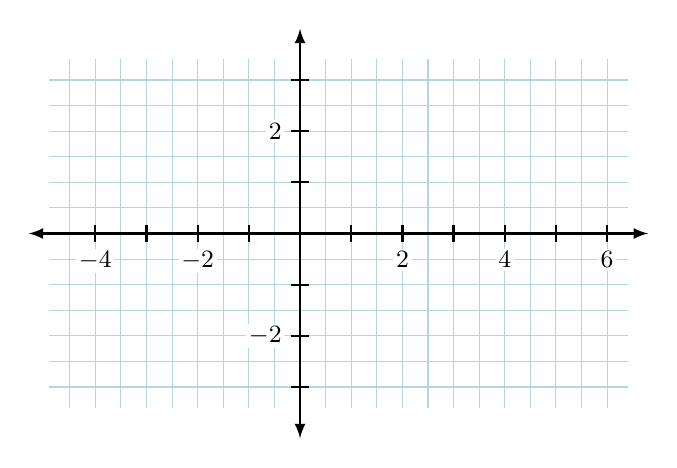
\begin{tikzpicture}[xscale=.65,yscale=.65]
    \draw[step=.5,style=help lines,] (-4.9,-3.4) grid (6.4,3.4);
    \draw[latex-latex, thick] (-5.3,0)--(6.8,0);
    \draw[latex-latex, thick] (0,-4)--(0,4);
    \foreach \x in {-4,-2,2,4,6}
        \draw[thick] (\x,5pt) -- (\x,-5pt) node [below=.7mm,fill=white,inner sep=1pt] {\small$\x$};
    \foreach \y in {-2,2}
        \draw[thick] (5pt,\y) -- (-5pt,\y) node [left=.7mm,fill=white,inner sep=1pt] {\small$\y$};
    \foreach \x in {-3,-1,1,3,5}
        \draw[thick] (\x,5pt) -- (\x,-5pt);
    \foreach \y in {-3,3,-1,1}
        \draw[thick] (5pt,\y) -- (-5pt,\y);
\end{tikzpicture}

Now, eliminate the parameter to find the Cartesian equation of the curve.
\vspace{2cm}

Sketch the curve represented by $x=3\cos\theta$ and $y=4\sin\theta$, $0\le\theta\le2\pi$. Then, eliminate the parameter.

\begin{tikzpicture}[xscale=.65,yscale=.65]
    \draw[step=.5,style=help lines,] (-4.4,-4.4) grid (4.4,4.4);
    \draw[latex-latex, thick] (-4.5,0)--(4.5,0);
    \draw[latex-latex, thick] (0,-4.5)--(0,4.5);
    \foreach \x in {-4,-2,2,4}
        \draw[thick] (\x,5pt) -- (\x,-5pt) node [below=.7mm,fill=white,inner sep=1pt] {\small$\x$};
    \foreach \y in {-1,1,-3,3}
        \draw[thick] (5pt,\y) -- (-5pt,\y) node [left=.7mm,fill=white,inner sep=1pt] {\small$\y$};
    \foreach \x in {-3,-1,1,3}
        \draw[thick] (\x,5pt) -- (\x,-5pt);
    \foreach \y in {-2,2,-4,4}
        \draw[thick] (5pt,\y) -- (-5pt,\y);
\end{tikzpicture}




\newpage
\phantomsection\addcontentsline{toc}{section}{Polar, Parametric, \& Vector Equations}
\phantomsection\addcontentsline{toc}{subsection}{Parametric Equations \& Calculus}
\subsection*{Parametric Equations and \& Calculus}
\begin{tcolorbox}[title= PARAMETRIC FORM OF THE DERIVATIVE,colframe=black,sharp corners,colback=white,colbacktitle=white,coltitle=black]

    If a smooth curve $C$ is given by the equations $x=f(t)$ and $y=g(t)$, then the slope of $C$ at the point $(x,\,y)$ is 
    \[\frac{dy}{dx}=\frac{dy/dt}{dx/dt},\,\,\,\frac{dx}{dt}\ne0.\]
    The second derivative (and every subsequent derivative) is
    \[\frac{d^2y}{dx^2}=\frac{d}{dx}\left[\frac{dy}{dx}\right]=\frac{\frac{d}{dt}\left[\frac{dy}{dx}\right]}{dx/dt}.\]
\end{tcolorbox}
\vspace{.1cm}
\textbf{Example:}
\begin{questions}
    \question Given the parametric equations $x=2\sqrt{t}$ and $y=3t^2-2t$, find $dy/dx$ and $d^2y/dx^2$.
    \vspace{\stretch{1}}

    \question Given the parametric equations $x=4\cos t$ and $y=3\sin t,$ write the equation of the tangent line to the curve at the point where $t=\frac{3\pi}{4}.$
    \vspace{\stretch{1}}

    \newpage 
    
    \question Find all points of vertical and horizontal tangency given the parametric equations $x=t^2+2,\,y=t^2-3t=5$.
    \vspace{\stretch{1}}

\end{questions}

\begin{tcolorbox}[title= PARAMETRIC FORM OF ARC LENGTH ,colframe=black,sharp corners,colback=white,colbacktitle=white,coltitle=black]

    If a smooth curve $C$ is given by the equations $x=f(t)$ and $y=g(t)$ such that $C$ does not intersect itself on the interval $(a,\,b)$, then the arc length of $C$ over the interval $(a,\,b)$ is given by: 
    \[L=\int_{a}^{b}\sqrt{\left(\frac{dx}{dt}\right)^2+\left(\frac{dy}{dt}\right)^2}\,dt.\]
    
\end{tcolorbox}
\vspace{.1cm}
A particle moves along a smooth curve given by $x=t^2+1$ and $y=4t^3-1$. How far did the particle travel between $t=0$ and $t=5$? BONUS: How far away is the particle from its starting position after the 5 seconds?
\vspace{\stretch{1}}


\newpage
\phantomsection\addcontentsline{toc}{subsection}{Vector Functions and Motion}
\subsection*{Vector Functions and Motion}
Parametric, Vector, and (eventually) Polar are all essentially the same. In this section, we introduce the form of a vector valued function, but you will see how it is essentially the same as a parametric one.

\begin{tcolorbox}[colframe=black,sharp corners,colback=white,boxrule=.25mm]
    \begin{center}
        \textbf{The Essentials}
    \end{center}
    
    \vspace{.7cm}
    
    If $\displaystyle\vec{r}(t)=\langle x(t),\,y(t)\rangle$ is the position vector of a particle moving along a smooth curve in the $xy$-plane, then, at any time $t$,
    \begin{enumerate}
        \item The particle's \textbf{velocity vector} $\displaystyle\vec{v}(t)=\langle x'(t),\,y'(t)\rangle$; if drawn from the position point, it is tangent to the points in the direction of increasing $t$.
        
        \item The particle's \textbf{speed} along the curve is the length (magnitude) of the velocity vector: \[\displaystyle\left|\vec{v}(t)\right|=\sqrt{x'(t)^2 +y'(t)^2}.\]
        
        \item The particle's \textbf{acceleration vector} $\displaystyle\vec{a}(t)=\langle x''(t),\,y''(t)\rangle$, is the derivative of the velocity vector and the second derivative of the position vector.
    \end{enumerate}
    
    \vspace{.5cm}
    
    If $\displaystyle\vec{v}(t)=\langle x'(t),\,y'(t)\rangle$ is the velocity vector of a particle moving along a smooth curve in the $xy$-plane, then
    \begin{enumerate}
        \item The \textbf{displacement} from $t=a$ to $t=b$ is given by the vector:
        \[\left\langle\int_a^b x'(t)\,dt,\,\int_a^b y'(t)\,dt\right\rangle\]
        The proceeding vector is added to the position at time $t=a$ to get the position at time $t=b$.
       
        \item The \textbf{distance traveled} from $t=a$ to $t=b$ is given by
        \[\int_a^b \left|\vec{v}(t)\right|\,dt=\int_a^b \sqrt{(x'(t))^2+(y'(t))^2}\,dt\]
        Note that this is just arc length for a parametric curve.
    \end{enumerate}
    
    
\end{tcolorbox}

\noindent\textbf{Examples:}
\begin{questions}
    \question A particle moves in the $xy$-plane so that at any time $t$, the position of the particle is given by $x(t)=t^3+2t^2,\,y(t)=t^4-t^3$.
    \begin{parts}
        \begin{minipage}[t]{.45\linewidth}
            \part Find the velocity vector when $t=1$.
        \end{minipage}
        \hfill
        \begin{minipage}[t]{0.45\linewidth}
            \part Find the $\vec{a}(t)$ when $t=2$.
        \end{minipage}
    \end{parts}


    \newpage

    \question A particle moves in the $xy$-plane so that at any time $t$, $t\ge0$, the position of the particle is given by $x(t)=t^2+3t,\,y(t)=t^3-3t^2$. Find the magnitude of the velocity vector when $t=1$.
    
    \vspace{\stretch{1}}

    \question A particle moves in the $xy$-plane so that its position is given by \[\displaystyle\vec{r}(t)=\left\langle\sqrt{3}-4\cos t,\,1-2\sin t\right\rangle,\]where $0\le t\le2\pi$. The path of the particle intersects the $x$-axis twice. Write an expression that represents the distance traveled by the particle between the two $x$-intercepts. Do no evaluate.
    
    \vspace{\stretch{1}}
    
    \question A particle moves with a velocity vector of $\langle3t^2-4t,\,8t^3+5\rangle.$ If the position vector at $t=0$ is $\langle7,\,-4\rangle$, find the position of the particle at $t=1$.
    
    \vspace{\stretch{1}}
    
\end{questions}


\newpage
\phantomsection\addcontentsline{toc}{subsection}{Polar Coordinates and Graphs}
\subsection*{Polar Coordinates and Graphs}

\begin{center}
        \underline{A Quick Review}
\end{center}
\begin{minipage}[t]{0.45\linewidth}
    Plot the following points:\\
    \begin{questions}
        \question $\displaystyle A\left(3,\frac{7\pi}{6}\right)$
        \vspace{1cm}
        
        \question $\displaystyle B\left(-2,\frac{5\pi}{4}\right)$
        \vspace{1cm}
        
        \question $\displaystyle C\left(2,\frac{-\pi}{6}\right)$
        \vspace{1cm}
        
        \question $\displaystyle D\left(-3,\,-3\pi\right)$
        
    \end{questions}
    
\end{minipage}
\hfill
\begin{minipage}[t]{0.45\linewidth}
    \begin{tikzpicture}[>=latex,baseline=(current bounding box.north)]
        % Draw the lines at multiples of pi/12
        \foreach \ang in {0,...,31} {
          \draw [lightgray] (0,0) -- (\ang * 180 / 16:4);
        }
        
        % Add the labels at multiples of pi/4
        \foreach \ang/\lab/\dir in {
          0/0/right,
          1/{\pi/4}/{above right},
          2/{\pi/2}/above,
          3/{3\pi/4}/{above left},
          4/{\pi}/left,
          5/{5\pi/4}/{below left},
          7/{7\pi/4}/{below right},
          6/{3\pi/2}/below} {
          \draw (0,0) -- (\ang * 180 / 4:4.1);
          \node [fill=white] at (\ang * 180 / 4:4.2) [\dir] {\scriptsize $\lab$};
        }
        
        % Concentric circles and radius labels
        \foreach \s in {0, 1, 2, 3} {
          \draw [lightgray] (0,0) circle (\s + 0.5);
          \draw (0,0) circle (\s);
          \node [fill=white] at (\s, 0) [below=1mm,inner sep=1pt] {\scriptsize $\s$};
        }
        
        
        
        % The double-lined circle around the whole diagram
        \draw [style=double] (0,0) circle (4);
    \end{tikzpicture}
\end{minipage}

\begin{tcolorbox}[title= COORDINATE CONVERSION EQUATIONS ,colframe=black,sharp corners,colback=white,colbacktitle=white,coltitle=black]

    

    Let the point $P$ have polar coordinates $(r,\,\theta)$ and rectangular coordinates $(x,\,y)$. Then
    \begin{minipage}[t]{.45\linewidth}
        \[x=r\cos \theta\]
    \end{minipage}
    \hfill
    \begin{minipage}[t]{.45\linewidth}
        \[y=r\sin \theta\]
    \end{minipage}
    
    \begin{minipage}[t]{.45\linewidth}
        \[r^2=x^2+y^2\]
    \end{minipage}
    \hfill
    \begin{minipage}[t]{.45\linewidth}
        \[\tan\theta=\frac{y}{x}\]
    \end{minipage}
    
\end{tcolorbox}
\vspace{.1cm}
\noindent\textbf{Examples:} Convert the following points/equations to the other coordinate system.
\begin{questions}
    \begin{minipage}{.45\linewidth}
        \question $\displaystyle\left(2,\,\frac{5\pi}{6}\right)$
    \end{minipage}
    \hfill
    \begin{minipage}{0.45\linewidth}
        \question $\displaystyle (3,\,-3)$
    \end{minipage}
    
    \newpage
    
    \begin{minipage}{0.45\linewidth}
        \question $y=4$
    \end{minipage}
    \hfill
    \begin{minipage}{0.45\linewidth}
        \question $x^2+y^2=25$
    \end{minipage}
    
    \vspace{\stretch{1}}
    
    \begin{minipage}{0.45\linewidth}
        \question $r\sin\theta=3$
    \end{minipage}
    \hfill
    \begin{minipage}{0.45\linewidth}
        \question $\displaystyle\theta=\frac{2\pi}{3}$
    \end{minipage}

    \vspace{\stretch{1}}    
    
\end{questions}

\textbf{Graphing:}
\begin{questions}
    \begin{minipage}{0.45\linewidth}
        \question $r=2\cos3\theta$\\
        \\
        \begin{tikzpicture}[>=latex,baseline=(current bounding box.north),scale=.7]
            % Draw the lines at multiples of pi/12
            \foreach \ang in {0,...,31} {
              \draw [lightgray] (0,0) -- (\ang * 180 / 16:4);
            }
            
            % Add the labels at multiples of pi/4
            \foreach \ang/\lab/\dir in {
              0/0/right,
              1/{\pi/4}/{above right},
              2/{\pi/2}/above,
              3/{3\pi/4}/{above left},
              4/{\pi}/left,
              5/{5\pi/4}/{below left},
              7/{7\pi/4}/{below right},
              6/{3\pi/2}/below} {
              \draw (0,0) -- (\ang * 180 / 4:4.1);
              \node [fill=white] at (\ang * 180 / 4:4.2) [\dir] {\scriptsize $\lab$};
            }
            
            % Concentric circles and radius labels
            \foreach \s in {0, 1, 2, 3} {
              \draw [lightgray] (0,0) circle (\s + 0.5);
              \draw (0,0) circle (\s);
              \node [fill=white] at (\s, 0) [below=1mm,inner sep=1pt] {\scriptsize $\s$};
            }
            
            
            
            % The double-lined circle around the whole diagram
            \draw [style=double] (0,0) circle (4);
        \end{tikzpicture}
    \end{minipage}
    \hfill
    \begin{minipage}{0.45\linewidth}
        \question $r=2(1-\cos\theta)$\\
        \\
        \begin{tikzpicture}[>=latex,baseline=(current bounding box.north),scale=.7]
            % Draw the lines at multiples of pi/12
            \foreach \ang in {0,...,31} {
              \draw [lightgray] (0,0) -- (\ang * 180 / 16:4);
            }
            
            % Add the labels at multiples of pi/4
            \foreach \ang/\lab/\dir in {
              0/0/right,
              1/{\pi/4}/{above right},
              2/{\pi/2}/above,
              3/{3\pi/4}/{above left},
              4/{\pi}/left,
              5/{5\pi/4}/{below left},
              7/{7\pi/4}/{below right},
              6/{3\pi/2}/below} {
              \draw (0,0) -- (\ang * 180 / 4:4.1);
              \node [fill=white] at (\ang * 180 / 4:4.2) [\dir] {\scriptsize $\lab$};
            }
            
            % Concentric circles and radius labels
            \foreach \s in {0, 1, 2, 3} {
              \draw [lightgray] (0,0) circle (\s + 0.5);
              \draw (0,0) circle (\s);
              \node [fill=white] at (\s, 0) [below=1mm,inner sep=1pt] {\scriptsize $\s$};
            }
            
            
            
            % The double-lined circle around the whole diagram
            \draw [style=double] (0,0) circle (4);
        \end{tikzpicture}
    \end{minipage}
\end{questions}
    
    


\newpage
\phantomsection\addcontentsline{toc}{subsection}{Polar Equations \& Calculus}
\subsection*{Polar Equations \& Calculus}

\begin{tcolorbox}[title= SLOPE IN POLAR FORM ,colframe=black,sharp corners,colback=white,colbacktitle=white,coltitle=black]

    %f to r in definition
    
    If $r$ is a differentiable function of $\theta$, then the slope of the tangent line to the graph of $r=f(\theta)$ at the point $(r,\,\theta)$ is
    \[\frac{dy}{dx}=\frac{dy/d\theta}{dx/d\theta}=\frac{r\cos\theta+r'\sin\theta}{-r\sin\theta+r'\cos\theta}\]
    provided that $dx/d\theta\ne0$ at $(r,\,\theta)$.
    
\end{tcolorbox}
\vspace{.1cm}

From this, we get two main deductions:
\begin{enumerate}
    \item Solutions to $\displaystyle\frac{dy}{d\theta}=0$ yield horizontal tangents so long as $\displaystyle\frac{dx}{d\theta}\ne0$
    \item Solutions to $\displaystyle\frac{dx}{d\theta}=0$ yield vertical tangents so long as $\displaystyle\frac{dy}{d\theta}\ne0$
\end{enumerate}
\noindent\textbf{Examples:}
\begin{questions}
    \question Find $\frac{dy}{dx}$ and the slope of the polar curve $r=3+2\sin\theta$ at $\theta=\pi/6$.
    \vspace{\stretch{1}}
    
    \question Find all of the vertical and horizontal tangents to the graph of $r=2(1-\cos\theta)$.
    \vspace{\stretch{1}}
    
    \question (Calculator) Sketch the graph of $r=2\csc\theta+5$. Find all points of horizontal and vertical tangency.
    \vspace{\stretch{.7}}
\end{questions}


\newpage
\phantomsection\addcontentsline{toc}{subsection}{Polar Area}
\subsection*{Polar Area}
\begin{tcolorbox}[title= AREA IN POLAR FORM ,colframe=black,sharp corners,colback=white,colbacktitle=white,coltitle=black]

    If $f$ is a continuous and nonnegative on the interval $[\alpha,\,\beta]$, $0<\beta-\alpha\le2\pi$, then the area of the region bounded by the graph of $r=f(\theta)$ is given by
    \begin{align*}
        A   &= \frac{1}{2}\int_\alpha^\beta[f(\theta)]^2\,d\theta\\
            &= \frac{1}{2}\int_\alpha^\beta r^2\,d\theta
    \end{align*}
    
\end{tcolorbox}
\vspace{.1cm}
\noindent\textbf{Examples:} Use a calculator for all of the following.
\begin{questions}
    \question Find the area bounded by the graph of $r=2+2\sin\theta.$
    \vspace{\stretch{1}}
    
    \question Find the area of one petal of $r=2\sin3\theta$.
    \vspace{\stretch{1}}
    
    \question Find the area of one petal of $r=4\cos2\theta$.
    \vspace{\stretch{1}}
    
    \newpage
    
    \question Find the area of the inner loop of the graph of $r=1+2\sin\theta$.
    \vspace{\stretch{1}}
    
    \question Find the area of the graph of $r=1+2\sin\theta$
    \vspace{\stretch{1}}
    
    \question Find the area between the two loops of the graph $r=1+2\sin\theta$.
    \vspace{\stretch{1}}
    
    \newpage
    
    \question Find the area inside $r=3\sin\theta$ and outside $r=2-\sin\theta$.
    \vspace{\stretch{1}}
    
    \question Find the area of the common interior of $r=3\cos\theta$ and $r=1+\cos\theta$.
    \vspace{\stretch{1}}
\end{questions}

\newpage

\hspace{0pt}
\vfill
\begin{center}
    \textbf{The End}
\end{center}
\vfill
\hspace{0pt}


\newpage



%% add cram sheet or something like it to appendix

%% add series tests summary to end of book

\phantomsection\addcontentsline{toc}{section}{Appendix}
\phantomsection\addcontentsline{toc}{subsection}{Hierarchy of Functions}


\begin{center}
    \textbf{\Huge Hierarchy of Functions}
\end{center}

\vspace{\stretch{1}}

\noindent We consider how fast different types of functions approach infinity. Here, assume that $c\in\mathbb{R}^+$ and $x\to\infty$.
\[...<\ln(\ln(x))<\ln(x)<x^{1/c}<x<x^c<c^x<x!<x^x<x^{x^x}<...\]

\begin{center}
\begin{tikzpicture}[domain=0:20, xscale=2/3, yscale=2/3]
  \draw[very thin,color=gray] (-0.1,-1.1) grid (19.9,19.9);
  \draw[->] (-0.2,0) -- (20.2,0) node[right] {$x$};
  \draw[->] (0,-1.2) -- (0,20.2) node[above] {$f(x)$};
  \draw[color=black!50!green] plot (\x, \x) node[right] {$x$};
  \draw[color=orange, domain=0:ln(20)] plot (\x, {exp(\x) })
    node[above right] {$\mathrm e^{x}$};
  \draw[color=purple,domain=1/e:20, smooth] plot (\x,{ln(\x)}) node[right] {$\ln(x)$};
  \draw[color=yellow!60!orange, domain=0:sqrt(20)] plot (\x, {\x*\x}) node[above right] {$x^2$};
  \draw[domain=e^(1/e):20, smooth] plot (\x,{ln(ln(\x))}) node[right] {$\ln(\ln(x))$};
  \draw[color=red,smooth, domain=0:2.855330859]
  plot (\x,{\x^(\x)}) node[above left]{$x^x$};
  \draw[color=blue, smooth] plot (\x,{sqrt(\x)}) node[right]{$\sqrt{x}$};
  
  \draw[color=black!60!red] (0,1) node [circle,fill,color=black!50!red,inner sep=1pt]{} -- (1,1) node [circle,fill,color=black!50!red,inner sep=1pt]{};
  \draw[color=black!60!red] (1,1) node [circle,fill,color=black!50!red,inner sep=1pt]{} -- (2,2) node [circle,fill,color=black!50!red,inner sep=1pt]{};
  \draw[color=black!60!red] (2,2) [circle,fill,color=black!50!red,inner sep=1pt]{} -- (3,6) node [circle,fill,color=black!50!red,inner sep=1pt]{};
  \draw[color=black!60!red] (3,6) node [circle,fill,color=black!50!red,inner sep=1pt]{} -- (3.778,20) node [color=black!50!red, above right]{$x!$};
  
\end{tikzpicture}
\end{center}
\vspace{.2in}

\begin{center}
    The graph above shows some select examples of functions. Their growth helps us conceptualize certain limits involving their quotients.    
\end{center}

\vspace{\stretch{1}}

\newpage


\phantomsection\addcontentsline{toc}{subsection}{Definitions and Theorems}

\begin{multicols}{2}

\small

\RaggedRight

\entry{Continuity}{A function $f(x)$ is continuous at $x=a$ if all of the following are true: (i) $f(a)$ exists (ii) $\lim_{x\to a}f(x)$ exists (iii) $\lim_{x\to a}f(x)=f(a)$.}

\entry{Intermediate Value Theorem}{If function $f(x)$ is continuous on a closed interval $[a,\,b]$ and if $y$ is any number between $f(a)$ and $f(b)$, then there is at least one number $c\in[a,\,b]$ such that $f(c)=y$.}

\entry{Limit Theorem}{$\lim_{x\to a}f(x)=L$ if and only if $\lim_{x\to a^+}f(x)=L=\lim_{x\to a^-}f(x)$.}

\entry{Squeeze Theorem}{If $f(x)\le g(x)\le h(x)$ and $\lim_{x\to c}f(x)=\lim_{x\to c}h(x)=L$, then $\lim_{x\to c}g(x)=L)$.}

\entry{Definition of Derivative}{$f'(x)=\lim_{h\to0}\frac{f(x+h)-f(x)}{h}$ or $f'(x)=\lim_{x\to c}\frac{f(x)-f(c)}{x-c}$.}

\entry{Diff. - Cont. Theorem}{If a function is differentiable at $x=a$, then it is continuous at $x=a$.}

\entry{Mean Value Theorem}{If $f(x)$ is continuous on the closed interval $[a,\,b]$ and differentiable on the open interval $(a,\,b)$, then there is at least one number $c$ between $a$ and $b$ such that $f'(c)=\frac{f(b)-f(a)}{b-a}$.}

\entry{Average Value Theorem}{The average value of $f$ on $[a,\,b]$ is: $f_ave=\frac{1}{b-a}\int_a^b f(x)\,dx$.}

\entry{Derivative of Inverse}{$g'(c)=\frac{1}{f'(g(c))}$.}

\entry{Linearization}{$L(x)=f(a)+f'(a)(x-a)$.}

\entry{Critical Point}{A number $c$ in the domain of a function $f$ is a critical point of $f$ if either $f'(c)=0$ or DNE.}

\entry{Extrema}{Critical points that are either a local/absolute max/min.}

\entry{Point of Inflection}{Points of inflection of $f(x)$ are the point on the domain of $f$ where $f''(x)=0$ or DNE and $f''$ changes sign at that point.}

\entry{Extreme Value Theorem}{If $f$ is continuous on a closed interval $[a,\,b]$, then $f$ has both an absolute max and absolute min value on $[a,\,b]$.}

\entry{Fundamental Theorem of Calculus}{$\int_a^b f(x)\,dx=F(b)-F(a)$ and $\frac{d}{dx}\int_a^x f(t)\,dt=f(x)$.}

\entry{Position}{$s(t)=\int v(t)\,dt$.}

\entry{Velocity}{$v(t)=s'(t)$ or $v(t)=\int a(t)\,dt$.}

\entry{Acceleration}{$a(t)=v'(t)=s''(t)$.}

\entry{Speed}{$\text{Speed}=\|v(t)|=\sqrt{(x'(t))^2+(y'(t))^2}$. Speed increases when $v(t)$ and $a(t)$ have the same sign. Speed decreases when $v(t)$ and $a(t)$ have different signs.}

\entry{Total Distance}{Total Distance from time $a$ to $b$ is $\int_a^b |v(t)|\,dt$.}

\entry{Net Distance (Change)}{$\int _a^b v(t)\,dt$.}

\entry{Area in the Plane}{$A=\int_a^b(f(x)-g(x))\,dx$ where $f\ge g$ on $[a,\,b]$.}

\entry{Volume by Disks}{$V=\pi\int_a^b R^2\,dx$ (horizontal) or $V=\pi\int_c^d R^2\,dy$ (vertical).}

\entry{Volume by Washers}{$V=\pi\int_a^b (R^2-r^2)\,dx$ (horizontal) or $V=\pi\int_c^d (R^2-r^2)\,dy$ (vertical).}

\entry{Volume by Cross Sections}{$V=\pi\int_a^b A(x)\,dx$ (if perpendicular to $x$-axis) or $V=\pi\int_c^d A(y)\,dy$ (if perpendicular to $y$-axis).}

\entry{Arc Length}{$L=\int_a^b\sqrt{1+[f'(x)]^2}\,dx$ or $L=\int_c^d\sqrt{1+[f'(y)]^2}\,dy$.}

\entry{L'Hospital's Rule}{If $\lim_{x\to c}\frac{f}{g}$ is of the form $0/0$ or $\infty/\infty$, then $\lim_{x\to c}\frac{f}{g}=\lim_{x\to c}\frac{f'}{g'}$.}

\entry{Improper Integrals}{An integral $\int_a^b f(x)\,dx$ is improper if any bound is infinite or $f$ has at least one discontinuity on the interval $[a,\,b]$. Evaluate using limits.}

\entry{Parametric Slope}{$\frac{dy}{dx}=\frac{dy/dt}{dx/dt}$.}

\entry{Parametric 2nd Deriv.}{$\frac{d^2 y}{dx^2}=\frac{\frac{d}{dx}(dy/dx)}{dx/dt}$.}

\entry{Parametric Arc Length}{$L=\int_a^b\sqrt{[x'(t)]^2+[y'(t)]^2}\,dx$.}

\entry{Polar Slope}{$\frac{dy}{dx}=\frac{r\cos\theta+r'\sin\theta}{-r\sin\theta+r'\cos\theta}$.}

\entry{Polar Area}{$A=\frac{1}{2}\int_a^b r^2\,d\theta$ or $A=\frac{1}{2}\int_a^b (f(\theta))^2\,d\theta$.}

\entry{Area Between Polar Curves}{$A=\frac{1}{2}\int_a^b [R^2-r^2]\,d\theta$.}

\entry{Vector Position}{$s(t)=\langle x(t),\,y(t)\rangle$.}

\entry{Vector Velocity}{$v(t)=s'(t)=\langle x'(t),\,y'(t)\rangle$.}

\entry{Vector Acceleration}{$a(t)=v'(t)=s''(t)=\langle x''(t),\,y''(t)\rangle$.}

\entry{Vector Speed}{$|v(t)|=\sqrt{(x't)^2+(y'(t))^2}$.}


\end{multicols}

\vspace{.5 in}

\phantomsection\addcontentsline{toc}{subsection}{Series Tests Summary}

\begin{center}
    \textbf{\large Summary of Convergence Tests}
    
    \vspace{.2in}
    
    \qrcode{http://people.math.binghamton.edu/alex/EXAMS_PUBLIC/Convergence_Handout.pdf}
\end{center}

\vspace{\stretch{1}}

\phantomsection\addcontentsline{toc}{subsection}{A Quote}

\begin{center}
    \fbox{\fbox{\parbox{5.5in}{
    \textbf{A Quote:}\\
    Considering how many fools can calculate, it is surprising that it should be thought either a difficult or tedious task for any other fool to learn how to master the same tricks.\\ 
    
    Some calculus-tricks are quite easy. Some are enormously difficult. The fools who write the textbooks of advanced mathematics -- and they are mostly clever fools -- seldom take the trouble to show you how easy the easy calculations are. On the contrary, they seem to desire to impress you with their tremendous cleverness by going about it in the most difficult way.\\ 
    
    Being myself a remarkably stupid fellow, I have had to unteach myself the difficulties, and now beg to present to my fellow fools the parts that are not hard. \textbf{Master these thoroughly, and the rest will follow...}}}}
\end{center}


\vspace{\stretch{1}}

\end{document}